%% LLT: Turn off some annoying warnings...
\RequirePackage{silence}
\WarningFilter{titlesec}{Non standard sectioning command}
\WarningFilter{scrreprt}{Usage of package}
\WarningFilter{scrreprt}{Activating an ugly workaround}

% **************************************************
% Document Class Definition
% **************************************************
\documentclass[%
	paper=A4,					% paper size --> A4 is default in Germany
%	twoside=true,				% onesite or twoside printing
    oneside=true,
%	twoside=false,				% onesite or twoside printing
	openright,					% doublepage cleaning ends up right side
	parskip=full,				% spacing value / method for paragraphs
	chapterprefix=true,			% prefix for chapter marks
	12pt,						% font size
	headings=normal,			% size of headings
	bibliography=totoc,			% include bib in toc
	listof=totoc,				% include listof entries in toc
	titlepage=on,				% own page for each title page
	captions=tableabove,		% display table captions above the float env
	draft=false,				% value for draft version
]{scrreprt}%

\usepackage[onehalfspacing]{setspace}
\usepackage[ngerman]{babel} % Neue Deutsche Rechtschreibung
\usepackage[T1]{fontenc}
\usepackage{gensymb}
\usepackage[utf8]{inputenc}		% defines file's character encoding
\usepackage{paralist}          % for compactitem itemization
\usepackage{chngcntr}           % Einfache Nummerierung von Abbildungen
\counterwithout{figure}{chapter} % Einfache Nummerierung von Abbildungen
\usepackage{chngcntr}
\counterwithout{footnote}{chapter}
\usepackage{hyperref}
\newcommand\fnurl[2]{%
	\href{#2}{#1}\footnote{\url{#2}}%
}
\usepackage{graphicx}
\graphicspath{{/figuren/}}
\usepackage{float} % exaktes Figure Placement mit H
%\usepackage{listings} % Code Listings

%\lstset{
%  breaklines=true,
%%  numbers=left,
%  numbersep=5pt,
%  basicstyle=\footnotesize\ttfamily,
%  numberstyle=\tiny\color{black}
%%  literate=%
%%  {Ö}{{\"O}}1
%%  {Ä}{{\"A}}1
%%  {Ü}{{\"U}}1
%%  {ß}{{\ss}}2
%%  {ü}{{\"u}}1
%%  {ä}{{\"a}}1
%%  {ö}{{\"o}}1
%}
%\lstset{literate=
%  {á}{{\'a}}1 {é}{{\'e}}1 {í}{{\'i}}1 {ó}{{\'o}}1 {ú}{{\'u}}1
%  {Á}{{\'A}}1 {É}{{\'E}}1 {Í}{{\'I}}1 {Ó}{{\'O}}1 {Ú}{{\'U}}1
%  {à}{{\`a}}1 {è}{{\`e}}1 {ì}{{\`i}}1 {ò}{{\`o}}1 {ù}{{\`u}}1
%  {À}{{\`A}}1 {È}{{\'E}}1 {Ì}{{\`I}}1 {Ò}{{\`O}}1 {Ù}{{\`U}}1
%  {ä}{{\"a}}1 {ë}{{\"e}}1 {ï}{{\"i}}1 {ö}{{\"o}}1 {ü}{{\"u}}1
%  {Ä}{{\"A}}1 {Ë}{{\"E}}1 {Ï}{{\"I}}1 {Ö}{{\"O}}1 {Ü}{{\"U}}1
%  {â}{{\^a}}1 {ê}{{\^e}}1 {î}{{\^i}}1 {ô}{{\^o}}1 {û}{{\^u}}1
%  {Â}{{\^A}}1 {Ê}{{\^E}}1 {Î}{{\^I}}1 {Ô}{{\^O}}1 {Û}{{\^U}}1
%  {œ}{{\oe}}1 {Œ}{{\OE}}1 {æ}{{\ae}}1 {Æ}{{\AE}}1 {ß}{{\ss}}1
%  {ű}{{\H{u}}}1 {Ű}{{\H{U}}}1 {ő}{{\H{o}}}1 {Ő}{{\H{O}}}1
%  {ç}{{\c c}}1 {Ç}{{\c C}}1 {ø}{{\o}}1 {å}{{\r a}}1 {Å}{{\r A}}1
%  {€}{{\EUR}}1 {£}{{\pounds}}1
%}
%\usepackage{color}
%\definecolor{javared}{rgb}{0.6,0,0} % for strings
%\definecolor{javagreen}{rgb}{0.25,0.5,0.35} % comments
%\definecolor{javapurple}{rgb}{0.5,0,0.35} % keywords
%\definecolor{javadocblue}{rgb}{0.25,0.35,0.75} % javadoc


\usepackage{color}
\usepackage{listings}
%\usepackage{courier} %caused problems for me

\lstloadlanguages{% Check Dokumentation for further languages ...
	C,
	C++,
	csh,
	Java
}

\definecolor{red}{rgb}{0.6,0,0} % for strings
\definecolor{blue}{rgb}{0,0,0.6}
\definecolor{green}{rgb}{0.3,0.5,0.29}
\definecolor{cyan}{rgb}{0.0,0.6,0.6}

\lstset{
	language=csh,
	basicstyle=\footnotesize\ttfamily, 
	numbers=left, 
	numberstyle=\tiny, 
	numbersep=5pt, 
	tabsize=2, 
	extendedchars=true, 
	breaklines=true, 
	frame=b,
	stringstyle=\color{blue}\ttfamily, 
	showspaces=false, 
	showtabs=false, 
	xleftmargin=17pt,
	framexleftmargin=17pt,
	framexrightmargin=5pt,
	framexbottommargin=4pt,
	commentstyle=\color{green},
	morecomment=[l]{//}, %use comment-line-style!
	morecomment=[s]{/*}{*/}, %for multiline comments
	showstringspaces=false, 
	morekeywords={  abstract, event, new, struct,
		as, explicit, null, switch,
		base, extern, object, this,
		bool, false, operator, throw,
		break, finally, out, true,
		byte, fixed, override, try,
		case, float, params, typeof,
		catch, for, private, uint,
		char, foreach, protected, ulong,
		checked, goto, public, unchecked,
		class, if, readonly, unsafe,
		const, implicit, ref, ushort,
		continue, in, return, using,
		decimal, int, sbyte, virtual,
		default, interface, sealed, volatile,
		delegate, internal, short, void,
		do, is, sizeof, while,
		double, lock, stackalloc,
		else, long, static,
		enum, namespace, string},
	keywordstyle=\color{cyan},
	identifierstyle=\color{black},
}
\usepackage{caption}
\DeclareCaptionFont{white}{\color{white}}
\DeclareCaptionFormat{listing}{\colorbox{blue}{\parbox{\textwidth}{\hspace{15pt}#1#2#3}}} %changed \colorbox{8} to \colorbox{blue} cause 8 is not a color!
\captionsetup[lstlisting]{format=listing,labelfont=white,textfont=white, singlelinecheck=false, margin=0pt, font={bf,footnotesize}}



% **************************************************
% Debug LaTeX Information
% **************************************************
%\listfiles

% **************************************************
% Information and Commands for Reuse
% **************************************************
\newcommand{\thesisTitle}{Bachelorarbeit}
\newcommand{\thesisName}{Ibrahim Khaled Reguieg}
\newcommand{\thesisSubject}{Konzeption und prototypische Implementierung von innovativen Interaktionsmöglichkeiten mit Industriemaschinen in der virtuellen Realität im Kontext von Industrie 4.0}
\newcommand{\thesisDate}{\today}
%\newcommand{\thesisVersion}{Final}

\newcommand{\thesisFirstReviewer}{Prof. Dr. Kristian Hildebrand}
\newcommand{\thesisFirstReviewerUniversity}{\protect{Beuth Hochschule für Technik Berlin}}
\newcommand{\thesisFirstReviewerDepartment}{Fachbereich VI - Informatik und Medien}

\newcommand{\thesisSecondReviewer}{Prof. Dr. Felix Gers}
\newcommand{\thesisSecondReviewerUniversity}{\protect{Beuth Hochschule für Technik Berlin}}
\newcommand{\thesisSecondReviewerDepartment}{Fachbereich VI - Informatik und Medien}

%\newcommand{\thesisFirstSupervisor}{Jane Doe}
%\newcommand{\thesisSecondSupervisor}{John Smith}

%\newcommand{\thesisUniversity}{\protect{Praktikum beim Deutschen Forschungszentrum für Künstliche Intelligenz}}
%\newcommand{\thesisUniversityDepartment}{Forschungsgruppe Sprachtechnologien (DFKI-LT)}
%\newcommand{\thesisUniversityInstitute}{Projekt ``Smart Data for Mobility'' (SD4M)}
%\newcommand{\thesisUniversityGroup}{Clean Thesis Group (CTG)}
\newcommand{\thesisUniversityCity}{Berlin}
%\newcommand{\thesisUniversityStreetAddress}{Street address}
%\newcommand{\thesisUniversityPostalCode}{Postal Code}

% **************************************************
% Load and Configure Packages
% **************************************************

\usepackage[ngerman]{babel} % babel system, adjust the language of the content

\usepackage[					% clean thesis style
%	bibencoding=utf8,%
	figuresep=colon,%
	sansserif=false,%
	hangfigurecaption=false,%
	hangsection=true,%
	hangsubsection=true,%
	colorize=full,%
	colortheme=bluemagenta,%
% LLT: Use biber if using UTF8 encoding
%	bibsys=bibtex,%
	bibsys=biber,%
	bibfile=bib-refs,%
	bibstyle=alphabetic,%
]{cleanthesis}

\hypersetup{					% setup the hyperref-package options
	pdftitle={\thesisTitle},	% 	- title (PDF meta)
	pdfsubject={\thesisSubject},% 	- subject (PDF meta)
	pdfauthor={\thesisName},	% 	- author (PDF meta)
	plainpages=false,			% 	-
	colorlinks=false,			% 	- colorize links?
	pdfborder={0 0 0},			% 	-
	breaklinks=true,			% 	- allow line break inside links
	bookmarksnumbered=true,		%
	bookmarksopen=true			%
}

% **************************************************
% Document CONTENT
% **************************************************
\begin{document}

% --------------------------
% rename document parts
% --------------------------
\renewcaptionname{ngerman}{\figurename}{Abb.}
\renewcaptionname{ngerman}{\tablename}{Tab.}
%\renewcaptionname{english}{\figurename}{Fig.}
%\renewcaptionname{english}{\tablename}{Tab.}

% --------------------------
% Front matter
% --------------------------
\pagenumbering{roman}			% roman page numbing (invisible for empty page style)
\pagestyle{empty}				% no header or footers
% !TEX root = ../thesis-example.tex
% ------------------------------------  --> main title page
\begin{titlepage}
	\pdfbookmark[0]{titlepage}{titlepage}
	\tgherosfont
	\centering

%	{\large \thesisUniversity} \\[4mm]
	\includegraphics[width=0.5\linewidth]{figuren/Beuth} \\[2mm]
%	\textsf{\thesisUniversityDepartment} \\
%	\textsf{\thesisUniversityInstitute} \\[5mm]
%	\textsf{\thesisUniversityGroup} \\
%    {\normalsize DFKI Projektbüro Berlin}\\
%    {\normalsize Alt-Moabit 91c}\\
%    {\normalsize 10559 Berlin}\\[5mm]
%    {\small{Zeitraum 15.02.2016 - 07.05.2016 (12 Wochen)}}
	{\small \thesisFirstReviewerDepartment}\\[5mm]
	\vfill
	{\LARGE \color{ctcolortitle}\textbf{\thesisSubject}}\\[10mm]
	
	{\large \thesisName} \\[5mm]
    {\normalsize Matrikelnummer 813812} \\
	{\normalsize Studiengang Bachelor Medieninformatik} \\
    {\normalsize 6. Fachsemester} \\
    {\normalsize Beuth Hochschule für Technik Berlin} \\
	{\small E-Mail: Khaled.Reguieg@gmail.com} \\
	
	\vfill
	\begin{minipage}[t]{.27\textwidth}
		\raggedleft
		\textit{Betreuer}
	\end{minipage}
	\hspace*{15pt}
	\begin{minipage}[t]{.65\textwidth}
		{\large \thesisFirstReviewer} \\
	  	{\small \thesisFirstReviewerDepartment} \\[-1mm]
		{\small \thesisFirstReviewerUniversity}
	\end{minipage} \\[5mm]
	\begin{minipage}[t]{.27\textwidth}
		\raggedleft
		\textit{Gutachter}
	\end{minipage}
	\hspace*{15pt}
	\begin{minipage}[t]{.65\textwidth}
		{\large \thesisSecondReviewer} \\
	  	{\small \thesisSecondReviewerDepartment} \\[-1mm]
		{\small \thesisSecondReviewerUniversity}
	\end{minipage} \\[10mm]
	\thesisDate \\
\end{titlepage}		% INCLUDE: all titlepages
\cleardoublepage

\setcounter{tocdepth}{4}		% define depth of toc
\tableofcontents				% display table of contents
\cleardoublepage

\listoffigures
\cleardoublepage
\listoftables
\cleardoublepage

% --------------------------
% Body matter
% --------------------------
\pagenumbering{arabic}			% arabic page numbering
\setcounter{page}{1}			% set page counter
\pagestyle{maincontentstyle} 	% fancy header and footer

\chapter{Einführung}
Die rasanten Entwicklungen der Technologisierung und Digitalisierung haben branchenübergreifend einen Paradigmenwechsel eingeläutet. Die Konsequenz: Geräte wie beispielsweise Smartphones sind rund um die Uhr in sämtlichen Lebens- und Arbeitsbereichen aktiv, online und miteinander vernetzt. Digitale Geräte finden Einsatz im täglichen Leben und Arbeiten und so steht die Gesellschaft derzeit an der Schwelle zur vierten Industriellen Revolution.
%\fnurl{}{https://de.statista.com/statistik/daten/studie/309656/umfrage/prognose-zur-anzahl-der-smartphone-nutzer-weltweit/}

Damit einhergehend dringen neue Technologien, wie \textit{Virtual Reality} (VR) und \textit{Augmented Reality} (AR) in die globalen Märkte ein und beginnen die Entertainmentindustrie und die Arbeitswelt nachhaltig zu verändern. Durch die zunehmende Medienkompetenz und Offenheit der Gesellschaft ist die Bereitschaft vorhanden, neue Technologien zu nutzen. Es besteht daher ein hohes Interesse daran, geeignete Interaktionsmöglichkeiten für Aktionen im virtuellen Raum zu finden und zu erproben.
Das folgende Szenario verdeutlicht den Sachverhalt anhand einer Baumaschine und eines Maschinenführers im augmentierten Raum und stellt einen Rahmen für die prototypische Implementierung dar.
\paragraph*{Szenario der Anwendung}
Ein Maschinenführer befähigt eine Baumaschine mit Hilfe der Standard-Gesten der \textit{Microsoft HoloLens}, schwere reale Objekte von einer Position A zu Standort B zu befördern. Maschinen können heutzutage ohne weiteres Befehle von außen empfangen. Somit könnte der Maschinenführer die Maschine bequem und sicher in einer in 3D abstrahierten Replikation der Baustelle, die er in seiner Datenbrille sieht, bedienen. Er interagiert dann mit virtuellen Replikationen statt mit den echten Objekten auf der Baustelle. Die Interaktion mit den virtuellen Objekten wird über eine Netzwerkverbindung auf den Roboter übertragen, welcher dann das echte Objekt auf der realen Baustelle bewegt. Als Einsatzorte bieten sich menschenfeindliche Arbeitsumgebungen an, beispielsweise die Atmosphäre eines anderen Planeten, verseuchte oder unwegsame Gebiete der Erde oder das All.
In einer Arbeitsumgebung, in der nur Maschinen anwesend sind, kann kein Mensch zu Schaden kommen. Die Arbeiter wären keinen Witterungen oder gesundheitsgefährdenden Arbeitsumfeldern ausgesetzt. Resultat dessen wäre zwangsläufig weniger körperliche Erschöpfung, was wiederum weniger krankheitsbedingte Ausfälle der Maschinenführer bedeutet.
Die Interaktionsmöglichkeit mit den Maschinen wäre stets gegeben, so bleibt der menschliche Faktor, der alle Prozesse individuell der Situation anpassen kann, weiterhin gegeben und die Baustelle weiterhin wirtschaftlich.
\paragraph*{Fragestellung}
Aus diesem Szenario resultieren verschiedene Fragestellungen. Allen voran die Frage danach, wie der Mensch \frqq Herr der Maschinen\flqq\ bleiben kann. Welche Technologien eignen sich dazu, die Maschinenprozesse zu überwachen und zu beobachten? Und welche Interaktionen eignen sich am besten, einer Maschine Befehle zu erteilen, sowohl als Teleoperator als auch in enger räumlicher Zusammenarbeit mit der Maschine?

Um diese Fragen beantworten zu können, werden im Rahmen der vorliegenden Arbeit ein Konzept und eine prototypische Implementierung einer Industriemaschine im virtuellen Raum erstellt. Die Applikation wird mit innovativen Interaktionen bestückt und die Anwendung im Kontext der Industrie 4.0 diskutiert.

\section{Motivation und Kurzbeschreibung}
Innovative Ideen, Konzepte und Produkte zeichnen die Informatik und IT-Branche aus wie keine andere. So gilt es stets, neue Technologien zu erforschen, zu erlernen und frühzeitig Anwendungen und Konzepte auszuarbeiten, welche die Gesellschaft nachhaltig verändern können. Fast kein Industriezweig bleibt unberührt von diesen neuartigen, agilen Methoden und Konzepten. Datenbrillen, seien es nun VR oder AR \textit{Head-Mounted Display} (HMD) sind in ihrer \textit{Consumerversion} beziehungsweise als \textit{Development-Kit} auf den Märkten verfügbar. Noch sind sie zwar teuer, allerdings haben erste Hersteller bereits Preissenkungen angekündigt. Steigende Verkaufszahlen deuten darauf hin, dass es der Traum vieler Menschen ist, eine Datenbrille zu besitzen, sei es zu Entertainmentzwecken oder, um Vorteile im Alltag und im Arbeitsleben zu genießen. Was im Comic-Band \frqq Batman of the Future\flqq\ noch futuristisch und utopisch klang, nämlich einen Roboter mit einer Datenbrille und Gesten fernzusteuern, ist heute Gegenstand zahlreicher Forschungen, wie auch dieser Arbeit. In einer Episode des Bandes benutzt einer der Akteure einen riesigen Roboter als Baumaschine. Er steuert ihn über eine Datenbrille und Gesten, wie in Abbildung \ref{fig:BotF_Datenbrille} zu sehen.\begin{figure}[ht]
	\centering
	\includegraphics[width=.75\textwidth]{figuren/billy}
	\caption{Datenbrille in \frqq Batman of the Future\flqq. Bildquelle: \cite{billy}.}
	\label{fig:BotF_Datenbrille}
\end{figure} Um die Gesellschaft auf künftige Technologien vorzubereiten bedarf es Anwendungen, die diese Neuerungen erforschen, in ansehnlichen Szenarien darstellen und mit gutem Design und vorausschauenden Konzepten die Berührungsängste mit ihnen minimieren.

%\includegraphics[width=1.0\textwidth]{figuren/golem}\vspace{1cm}
\section{Aufbau}
Ziel der vorliegenden Arbeit soll es sein, mit Hilfe eines Prototyps einen Ausblick darauf zu geben, wie Menschen in Zukunft mit Maschinen interagieren, was dabei zu beachten ist und welche Interaktionsformen sich für industrielle Zwecke besonders eignen. Im Anschluss an eine ausführliche Definition der grundlegenden Begrifflichkeiten im Kapitel~\ref{chapter:Grundlagen} erfolgt eine Analyse des aktuellen Forschungsstandes sowie eine Erörterung der Plausibilität der Fragestellung dieser Arbeit. Unter anderem wird in diesem Zuge auch erläutert, weshalb \textit{Microsofts HoloLens} und \textit{Legos EV3} geeignete Geräte für die prototypische Implementierung sind. Im Anschluss werden die Relevanz und die Potentiale der Technologien Robotik, Datenbrillen und AR für Forschungseinrichtungen, Industrieunternehmen und Technik-Enthusiasten erläutert und außerdem darauf eingegangen, inwieweit die \frqq Industrie 4.0\flqq\ als ganzheitliches Konzept dahinter steht. 

Danach wird in Kapitel~\ref{chapter:Konzeption} ein Konzept erarbeitet und präsentiert, welches sich damit auseinandersetzt, wie über eine Datenbrille in Form einer \textit{Microsoft HoloLens} eine Maschine, im prototypischen Fall ein Roboter aus \textit{Lego}, gesteuert und bei seiner Arbeit mit einem \textit{User Interface} augmentiert wird. Besagtes Vorhaben gilt es in Kapiel~\ref{chap:appImplementation} in einer Anwendung minimalisiert darzustellen und einen konzeptionellen Beweis dafür zu liefern, dass Interaktionen im virtuellen Raum auf die reale Welt übertragen werden können, einen Mehrwert bedeuten und dass sie im Kontext der vierten Industriellen Revolution eine Berechtigung besitzen. Abschließend wird diese These in Kapitel~\ref{chapter:UsabilityTest} mit einer benutzerbasierten, qualitativen Evaluation, dem \textit{Thinking-Aloud} Test, überprüft und dessen Ergebnisse ausgewertet.
\chapter{Grundlagen}\label{chapter:Grundlagen}
In diesem Kapitel wird erläutert, was der Begriff \frqq Industrie 4.0\flqq\  bedeutet, vor welche Herausforderungen sie uns stellt und welche Effekte mit ihr einhergehen. Des Weiteren behandelt dieses Kapitel grundlegende Sachverhalte bezüglich Fertigungsrobotern und dem hier als Substitution benutzten  \textit{Lego Mindstorms EV3} sowie Grundlagen zu AR und der genutzten Brille \textit{Microsoft HoloLens}.
\section{Industrie 4.0}\label{sec:i40}
Eine \frqq Industrielle Revolution\flqq\ bezeichnet \frqq einen raschen Wandel von Produktionstechniken und, daraus abgeleitet, von wirtschaftlich-gesellschaftlichen Strukturen.\flqq\footnote{ Prof. Dr. Voigt, 2016, [Accessed: 06.01.2017].} Die \frqq Industrie 4.0\flqq\ bezeichnet das Ergebnis der vierten \textit{Industriellen Revolution}. Sie reiht sich an der Spitze von drei Vorgängern ein:
\begin{itemize}
	\item Die erste \textit{Industrielle Revolution}, etwa um 1750, bei der Arbeits- und Kraftmaschinen die Industrialisierung und das Verhindern von Hungerkatastrophen ermöglichte.
	\item Die zweite \textit{Industrielle Revolution}, etwa um 1870, die Wohlstand durch arbeitsteilige Massenproduktion mit Hilfe elektrischer Energie schaffte.
	\item Und die dritte \textit{Industrielle Revolution}, seit circa 1960, welche durch Elektronik und IT automatisierungsgetriebene Rationalisierung sowie die variantenreiche Serienproduktion ermöglichte.\footnote{ Vgl. Dipl.-Ing. Jäger et al, 2015.}
\end{itemize}
Diese Entwicklung ist zusätzlich schematisch in Abbildung~\ref{fig:VerlaufIndustrie402} dargestellt.
\begin{figure}[ht]
	\centering
	\includegraphics[width=.8\textwidth]{figuren/Industrie-40-Definition-Stufen-Revolution-01}
	\caption{Verlauf Industrieller Revolutionen ab 1800 bis heute. Bildquelle: \cite{i40Verlauf}.}
	\label{fig:VerlaufIndustrie402}
\end{figure}
Der Begriff \frqq Industrie 4.0\flqq\ ist ursprünglich ein Projektname einer Arbeitsgruppe des Bundesministerium für Wirtschaft und Energie (BMWi). Es sind zahlreiche Beschreibungen zu finden, die sich sehr stark ähneln. Für die folgende Arbeit wird daher die Definition des BMWi beibehalten:
\begin{quote}
	\frqq In der Industrie 4.0 verzahnt sich die Produktion mit modernster Informations- und Kommunikationstechnik [...] (zu)
	%. Treibende Kraft dieser Entwicklung ist die rasant zunehmende Digitalisierung von Wirtschaft und Gesellschaft. Sie verändert nachhaltig die Art und Weise, wie zukünftig in Deutschland produziert und gearbeitet wird: Nach Dampfmaschine, Fließband, Elektronik und IT bestimmen nun 
	intelligente(n) Fabriken (sogenannte „Smart Factories“) [...]
	%die vierte industrielle Revolution. Technische Grundlage hierfür sind intelligente, digital vernetzte Systeme, mit deren Hilfe eine weitestgehend selbstorganisierte Produktion möglich wird: 
	Menschen, Maschinen, Anlagen, Logistik und Produkte kommunizieren und kooperieren in der Industrie 4.0 direkt miteinander. Produktions- und Logistikprozesse zwischen Unternehmen im selben Produktionsprozess werden intelligent miteinander verzahnt, um die Produktion noch effizienter und flexibler zu gestalten.
	
	So können intelligente Wertschöpfungsketten entstehen, die zudem alle Phasen des Lebenszyklus des Produktes miteinschließen -- von der Idee eines Produkts über die Entwicklung, Fertigung, Nutzung und Wartung bisn hin zum Recycling. [...] %Auf diese Weise können zum einen Kundenwünsche von der Produktidee bis hin zum Recycling einschließlich der damit verbundenen Dienstleistungen mitgedacht werden. Deshalb können Unternehmen leichter als bisher maßgeschneiderte Produkte nach individuellen Kundenwünschen produzieren. Die individuelle Fertigung und Wartung der Produkte könnte der neue Standard werden. Zum anderen können trotz individualisierter Produktion die Kosten der Produktion gesenkt werden.Durch die Vernetzung der Unternehmen der Wertschöpfungskette ist es möglich, nicht mehr nur einen Produktionsschritt, sondern die ganze Wertschöpfungskette zu optimieren. Wenn alle Informationen in Echtzeit verfügbar sind, kann ein Unternehmen z.B. frühzeitig auf die Verfügbarkeit bestimmter Rohstoffe reagieren [...] (und) Produktionsprozesse können unternehmensübergreifend so gesteuert werden, dass sie Ressourcen und Energie sparen.
	[...]\flqq\footnote{ BMWi, Hrsg., 2016, [Accessed: 06.01.2017].}
	%	URL: \url{http://www.plattform-i40.de/I40/Navigation/DE/Industrie40/WasIndustrie40/was-ist-industrie-40.html}.}
	%
	%	Insgesamt kann die Wirtschaftlichkeit der Produktion gesteigert, die Wettbewerbsfähigkeit der Industrie in Deutschland gestärkt und die Flexibilität der Produktion erhöht werden.
\end{quote}
Momentan eher als Marketingbegriff benutzt, fasst der Ausdruck \frqq Industrie 4.0\flqq\ sehr gut zusammen, wie die Produktion in Deutschland, aber auch weltweit, in Zukunft aussehen kann. Ein hochgerechnetes Investitionsvolumen von jährlich 40 Mrd. Euro in den nächsten fünf Jahren zeigt deutlich, dass vernetzte und intelligente Produktionsstätten ein Hauptanliegen der deutschen Industrie und Wirtschaft darstellen\footnote{ Vgl. Dr. Geissbauer / Schrauf / Koch / et al. (2016), S.7.}. Sie sind maßgeblich dafür verantwortlich, dass Deutschland seine Vorreiterrolle und sein Ansehen als Motor moderner, effizienter und qualitativ hochwertiger Industrieanlagen weltweit behaupten und weiter ausbauen kann.

%vgl. PricewaterhouseCoopers Aktiengesellschaft Wirtschaftsprüfungsgesellschaft, Dr. Geissbauer / Schrauf / Koch / et al, S.7, 2016}
%Marktforschungsunternehmens PriceWaterhouseCooper (PwC) und die des Fraunhofer-Institut für Produktionsanlagen und Konstruktionstechnik (IPK) gewählt: \glqq 
%\footnote{(PwC (Hrsg.), 2016, S.1)}
\subsection{Herausforderungen}\label{ssec:i40Challenges}
Deutschland ist, wie in Abbildung \ref{fig:EULabourPerHour} zu sehen, ein Hochlohnstandort. Eine maßgebliche Herausforderung ist daher: Die Produktion durch Innovationen profitabel im Inland zu betreiben, statt sie ins Ausland zu verlagern.

\begin{figure}[ht]
	\centering
	\includegraphics[width=1.\textwidth]{figuren/Estimated_hourly_labour_costs_2015}
	\caption{Durchschnittliche Arbeitskosten pro Stunde in Europa, 2015. Bildquelle: \cite{hochlohnstandort}.}
	\label{fig:EULabourPerHour}
\end{figure}

Des Weiteren zählt die Bundesrepublik Deutschland zu einem der Länder, dessen Rohstoffverlangen bei weitem die Menge dessen übersteigt, welche im Inland abgebaut werden kann. Es bilden sich Abhängigkeiten, um die Rohstoffversorgung zu sichern. Beispielsweise importierte die Bundesrepublik im Jahr 2005 Waren mit dem Gesamtwert von 625 Mrd. Euro, darunter 26,5 Mio. Tonnen Steinkohle und 110 Mio. Tonnen Rohöl.\footnote{ Topel / Seibel, Hrsg., o. J., [Accessed: 11.01.2017].}
Um wettbewerbsfähig und unabhängig zu sein, müssen die Produktionsstätten der Zukunft ressourcensparend und vor allem energieeffizient produzieren.
Hierzu gesellt sich auch das Schlagwort \frqq Urbane Produktion\flqq. Es bedeutet: \glqq das Umfeld einer Produktionsstätte in den Bilanzierungsrahmen der energetischen Optimierung einzubeziehen\grqq.\footnote{ Fraunhofer-Institut für Produktionstechnik und Automatisierung, Hrsg., o.J., [Accessed: 11.01.2017].} Dazu zählen sowohl Recycling als auch Abwärme und andere passive Rohstoffe.

Außerdem sehen sich Gesellschaften, die ein gewisses Maß an Wohlstand erreicht haben, mit einem demographischen Wandel konfrontiert.\footnote{ Vgl. Roser / Ortiz-Ospina, 2017, [Accessed: 01.02.2017].}
\begin{figure}[ht]
	\centering
	\includegraphics[width=1.\textwidth]{figuren/SOZ_01_04_Bevoelkerungsentwicklung_und_Altersstruktur}
	\caption{Bevölkerungsentwicklung in Deutschland von 1950-2050. Bildquelle: \cite{demographischerWandel}.}
	\label{fig:DEDemographischerWandel}
\end{figure}
In Abbildung~\ref{fig:DEDemographischerWandel} ist die Bevölkerungsentwicklung in Deutschland von 1950 bis 2050 zu sehen. Abzuleiten daraus ist, dass der Anteil der Bevölkerung im arbeitsfähigen Alter kleiner, und der nicht arbeitsfähige Anteil\footnote{ Vgl. Statistisches Bundesamt, Bevölkerung nach Altersgruppen, Hrsg., [Accessed: 11.01.2017].} größer wird. Dieser Wandel spannt verschiedene Problemfelder auf, deren Lösung von verschiedenen Seiten gefordert wird. Welche Lösungsansätze durch die \frqq4. Industrielle Revolution\flqq\ entstehen, wird im Folgenden erläutert.
\subsection{Effekte}\label{ssec:i40Effects}
Die aus den Herausforderungen resultierenden Effekte versucht die \frqq Industrie 4.0\flqq\ bewusst zu adressieren und anzugehen.
Intelligente Fabriken können das Arbeiten am Hochlohnstandort wieder profitabel machen. Das BMWi beschreibt diesen Wandel wie folgt: \glqq Industrie 4.0 bedeutet gute Arbeit, nicht menschenleere Fabriken. Vielmehr verändert sich das Arbeiten: Die Beschäftigten müssen stärker in die Prozesse eingebunden werden, zum Bespiel[sic] um Abläufe zu koordinieren, die Kommunikation zu steuern und eigenverantwortlich schnell Entscheidungen zu treffen\grqq.\footnote{ BMWi, Hrsg., 2016, [Accessed: 09.01.2017].}

Verzahnung von industrieller Produktion mit modernster Informations- und Kommunikationstechnik soll in hoher Individualität, Effizienz und Kostenersparnis münden. Schon heute ermöglichen Innovationen, wie beispielsweise ein intelligenter Handschuh\footnote{ Handschuh der beispielsweise Produktions- und Logistikprozesse verbessert und vereinfacht.}, Zeitersparnisse und mehr Effizienz im Logistiksektor. Eine \textit{Wearable}-Lösung wie diese begleitet einen Arbeiter auf dem Weg in die \frqq Industrie 4.0\flqq, ist jedoch eher in Logistik- und Zuliefererbetrieben anzusiedeln. Allerdings soll in Zukunft die Produktion durch \textit{Cyber Physical Systems}\footnote{ Cyber-Physische Systeme (CPS) sind Systeme mit eingebetteter Software und Elektronik, die über Sensoren und sogenannte Aktoren (Antriebselemente) mit der Außenwelt verbunden sind.} digitalisiert werden, damit dabei eine smarte Wertschöpfungskette entsteht, die ihren Energie- und Ressourcenbedarf optimal regulieren und ausschöpfen kann. Hinzukommend könnten Kreisläufe entstehen, die urbane Gegebenheiten, von Abwärme bis hin zu Recycling mit berücksichtigen und so die Produktionsprozesse noch umweltfreundlicher und effizienter gestalten.

Die Herausforderung einer alternden Gesellschaft bedeutet den Verlust von Arbeitskraft in menschlicher Form. Eine Industrielandschaft, in der Maschinen den Hauptteil der zu bewerkstelligenden Aufgaben erledigen können und nur ein vergleichsweise kleiner Teil der Gesellschaft durch fachliche Kompetenz diese Maschinen entwickeln und warten muss, kann einen solchen Wandel ausgleichen.

Diese Effekte durch gezielte Investitionen und Entwicklungen im Fachbereich der Sensorik und Robotik anzugehen, ist das Hauptanliegen der \frqq Industrie 4.0\flqq.\newpage
\section{Robotik}\label{sec:robots}
Die interdisziplinäre Kategorie der Robotik bezeichnet ein Teilgebiet des Ingenieurwesens, welches sich aus den Hauptbestandteilen Maschinenbau, Elektrotechnik und Informatik zusammensetzt und dessen Wortursprung im slawischen Wort \frqq robota\flqq\ liegt und soviel bedeutet wie \frqq Arbeiten\flqq.\footnote{ Vgl. Siciliano / Khatib, S.1, 2008.} 1920 wurde der Begriff vom tschechischen Schriftsteller Karel Čapeks in seinem Schauspiel \frqq R. U. R.\flqq\ (Rossums Universal-Roboter) im Sinne eines Maschinenmenschen erwähnt und dadurch geprägt. Die Robotik ist eine der Leitindustrien des 21. Jahrhunderts, woraus eine enge Verbindung zur Mensch-Maschine-Interaktion, Psychologie, Soziologie (soziale Robotik) und Philosophie (Maschinenethik) entsteht.\footnote{ Vgl. Prof. Dr. Bendel, Wirtschaftslexikon Stichwort: Robotik, o.J., o.S.}
\subsection{Überblick, Entwicklung und Forschungsstand}\label{ssec:researchRobots}
Der Verband Deutscher Ingenieure (VDI) definiert in seiner \textit{Richtlinie 2860} Roboter wie folgt: \frqq Industrieroboter sind universell einsetzbare Bewegungsautomaten mit mehreren Achsen, deren Bewegungen hinsichtlich Bewegungsfolge und Wegen bzw. Winkeln frei (d.h. ohne mechanischen bzw. menschlichen Eingriff) programmierbar und gegebenenfalls sensorgeführt sind. Sie sind mit Greifern, Werkzeugen oder anderen Fertigungsmitteln ausrüstbar und können Handhabungs- und/oder Fertigungsaufgaben ausführen\flqq.\footnote{ VDI-Richtlinie 2860, Blatt 1.}

Angefangen mit Heron von Alexandria (Abb. \ref{fig:Automata}) und seinen Entwürfen für ein Automatentheater um etwa 100 nach Christus, über die drei Droiden (Zeichner, Schriftsteller und Klavierspieler) aus Abbildung \ref{fig:jaquet}, gebaut 1774 von Jaquet Droz und dessen Sohn, bis zur Erfindung des Industrieroboters durch George Devol 1954 (Patentzeichnung in Abbildung \ref{fig:Devol_Patent}) sind Automaten dafür erdacht worden, den Menschen Arbeiten abzunehmen und sie durch die Automatisierung von Arbeitsschritten zu entlasten.\footnote{ Vgl. Prof. Dr.-Ing. Linemann, S.4 ff., 2016.}
\begin{figure}[H]
	\centering
	\includegraphics[width=0.5\textwidth]{figuren/Hero_of_Alexandria_Automata}
	\caption{Skizze von Heron von Alexandria \frqq Automata\flqq. Bildquelle: \cite{automata}.}
	\label{fig:Automata}
\end{figure}
\begin{figure}[H]
	\centering
	\includegraphics[width=1.\textwidth]{figuren/Jaquet}
	\caption{Die Droiden von Jaquet Droz und seinem Sohn: Der Zeichner (links) und seine Zeichnung (links unten), Der Schreiber (mitte) und dessen Text (rechts unten) und die Musikerin (rechts). Bildquelle: \cite{zeichner}, \cite{schreiber}, \cite{musikerin}, \cite{zeichnung}, \cite{text}.}
	\label{fig:jaquet}
\end{figure} 
\begin{figure}[H]
	\centering
	\includegraphics[width=.5\textwidth]{figuren/Devol_Patent_1954}
	\caption{Patentzeichnung für den ersten Industrieroboter. Bildquelle: \cite{devol}.}
	\label{fig:Devol_Patent}
\end{figure}
Laut der oben genannten VDI-Richtlinie sind Industrieroboter eine Untergruppe der Handhabungsgeräte. Abbildung \ref{fig:Handhabungsgeräte} zeigt dabei ihre Unterteilung in verschiedene Untergruppen. Zu erwähnen ist, dass die Kategorien \frqq Manipulator, Teleoperator\flqq\ und \frqq Industrieroboter\flqq\ in Zukunft wieder zusammengeführt werden könnten. So zählt auch in dieser Abschlussarbeit die prototypische Implementierung mehr zur Kategorie der Teleoperator. Allerdings wird darauf hingewiesen, dass Industrieroboter durch das verschmelzen der Arbeitsbereiche von Mensch und Maschine immer mehr zu \frqq Cobots\flqq\footnote{ Kooperierende Roboter (Cobot), bezeichnen Roboter die gemeinsam
	mit Menschen Arbeit verrichten.} werden könnten und somit ein hybrides Dasein zwischen Werkzeug und autonomer Maschine pflegen könnten.

\begin{figure}[H]
	\centering
	\includegraphics[width=.5\textwidth]{figuren/Handhabungsgeraete}
	\caption{Unterteilung von Handhabungsgeräten in Untergruppen. Bildquelle: \cite{pdf:roboticScript}.}
	\label{fig:Handhabungsgeräte}
\end{figure}
Man unterscheidet vier Hauptgruppen von Robotern:
\begin{itemize}
	\item Industrieroboter
	\item Serviceroboter
	\item Geländeroboter
	\item Autonome Roboter / Agentensysteme
\end{itemize}
Betrachtet man die Gruppe der Industrieroboter genauer, ist es wichtig sich über die genaue Beschaffenheit des Roboters im Klaren zu sein, da sie sowohl seinen Arbeitsraum als auch die Komplexität seiner Bewegungen definieren. Die Hauptkomponenten sind, wie in Abbildung \ref{fig:Roboter_Beschaffenheit} gezeigt, das Fahrzeug, welches die Lokomotion bestimmt, der Roboterarm, der den Endeffektor führt, und der Endeffektor selbst, welcher mit der Umwelt interagiert.
\begin{figure}[H]
	\centering
	\includegraphics[width=.5\textwidth]{figuren/Roboter_Beschaffenheit}
	\caption{Schematische Darstellung eines Industrieroboters. Bildquelle: \cite{pdf:roboticScript}.}
	\label{fig:Roboter_Beschaffenheit}
\end{figure}
Alle genannten Komponenten haben Freiheitsgrade, welche die Komplexität der Dynamik und Kinematik des Roboters festlegen. Die folgende Formel bestimmt dabei die Bewegungsfreiheitsgrade eines Roboters:
\begin{equation}
F=\sum_{i=1}^{n}(F_{R_{i}} + F_{T_{i}})\textrm{, mit }F \geq f
\end{equation}
Dabei gibt $F_{R}$ den Freiheitsgrad eines Rotationsgelenks an und nimmt einen Wert $\leq 3$ an, $F_{T}$ gibt den Freiheitsgrad eines Translationsgelenks an, der bei 1 liegt und n beschreibt die Anzahl der Gelenke eines Roboters.
\subsection{Fertigungsroboter}\label{ssec:industryRobots}
Das Bild der Fertigungsstraßen des frühen letzten Jahrhunderts korreliert mit dem Verlauf der Industriellen Revolutionen aus Abbildung \ref{fig:VerlaufIndustrie402}. Die Werkshallen waren bedingt durch Henry Fords Erfindung, der Bandfertigung, gefüllt mit Arbeitern, die zum Teil simple und monotone Arbeiten ausführen mussten (Abbildung.~\ref{fig:WerkshalleFord}).
\begin{figure}[H]
	\centering
	\includegraphics[width=1.\textwidth]{figuren/henry-ford-automobile}
	\caption{Fließbandarbeiter um 1913 in der Automobilfabrikation von Henry Ford. Bildquelle: \cite{ford}.}
	\label{fig:WerkshalleFord}
\end{figure}
Mit anhaltendem technologischen Fortschritt stieg auch die Anzahl der Arbeiten, die von Maschinen bewerkstelligt werden konnten. Maschinen die eine solche Aufgabe erfüllen, nennt man Fertigungsroboter. Beim Wort Roboter, haben viele Menschen das Bild eines \textit{Humanoiden Roboters}\footnote{ Roboter in Menschengestalt.}, wie er in Filmen oft zum Einsatz kommt, im Kopf. Allerdings sind Roboter in menschlicher Form nur bedingt sinnvoll, wenn es um das Lösen spezifischer Aufgaben geht, denn unsere Anatomie hindert uns an vielen Bewegungen. Das mag für uns sehr sinnvoll sein und kann physiologische Gründe haben, für einen Roboter mit einer bestimmten Aufgabe ist dies jedoch eher hinderlich. Warum sollte sich ein Roboterarm beispielsweise nicht in allen Freiheitsgraden bewegen können? Blickt man in die Produktionshallen des 21. Jahrhunderts sind dort in vielen Bereichen immer mehr solcher Roboter anzutreffen. Es scheint ein reges Interesse an Maschinen dieser Art zu herrschen.
\begin{figure}[ht]
	\centering
	\includegraphics[width=1.\textwidth]{figuren/Roboter_Werk}
	\caption{Industrieroboter in einem Daimler-Werk. Bildquelle: \cite{daimlerRoboter}.}
	\label{fig:WerkshalleDaimler}
\end{figure} Beispielsweise hat sich die Anzahl der Industrieroboter seit 2010 mehr als verdoppelt\footnote{ Vgl. Dr. Schmidt, S.5, 2016.} und chinesische Investoren haben letztes Jahr den deutschen Industrieroboterhersteller \textit{KUKA} gekauft.\footnote{ Süddeutsche Zeitung Hrsg., 2016, [Accessed: 16.02.2017].} Die Roboter erledigen ihre Aufgaben meist präziser und schneller als Menschen es je könnten, denn sie wurden für eine spezifische Aufgabe entwickelt und gebaut. Hinzu kommt, dass Roboter -- im Gegensatz zu Lebewesen -- nicht durch Krankheit oder persönliche Gründe ausfallen. So kann das ganze Jahr über eine gleichbleibend stabile Produktion und Qualität gewährleistet werden. Das führt allerdings auch dazu, dass Fertigungsroboter oft nur ihre eigenen Aufgaben kennen und nur wenige Sensoren zur Außenwelt besitzen. Betritt ein Mensch ihren Arbeitsbereich, ist höchste Vorsicht geboten, denn Industrieroboter sind schnell und kraftvoll; erkennt der Roboter den Menschen auf seinem Weg nicht, sind schwere Verletzungen bis hin zum Tod die Folge. Momentan arbeiten Roboter deswegen in einem Arbeitsbereich, der von dem des Menschen getrennt ist. In Zukunft soll sich dies durch immer leistungsfähigere, vernetzte und ihrer Umgebung gegenüber aufmerksamen Robotern ändern und das Arbeiten an der Fertigungsstraße von Mensch und Maschine kooperativ bewerkstelligt werden.
\subsection{Lego Mindstorms EV3}\label{ssec:legoMindstorms}
Der \textit{Lego Mindstorms EV3} ist die dritte Generation von einer Spielzeugreihe, die sich mit der Verwirklichung von Robotern oder technischen Maschinen aus \textit{Lego}-Steinen befasst. Es handelt sich dabei um einen größeren Stein, der als Rechner fungiert, und um Sensoren und Motoren, die per Kabel an diesen angeschlossen werden. Das Besondere daran ist: Man kann eigene Programme schreiben, welche die Motorenbewegung steuern und die Sensordaten auslesen. Mit grafischer Programmiersprache ausgeliefert, aber als Spielzeug für Kinder entwickelt und gedacht, erfreut sich der Stein auch in der Lehre und Forschung großer Beliebtheit. Tauscht man die Firmware des Steins aus, ist es möglich, diesen mit Programmen zu bespielen, die in \textit{Java}, \textit{C\#} oder \textit{Python} geschrieben wurden. Im Internet finden sich so unzählige Videos, Beiträge von Enthusiasten und Lehrbeispiele, welche die \textit{Mindstorms}-Reihe nutzen.
\begin{figure}[H]
	\centering
	\includegraphics[width=.75\textwidth]{figuren/ev3}
	\caption{Hauptkomponente des \textit{Lego Mindstorms} der \textit{EV3}-Stein. Bildquelle: \cite{ev3}.}
	\label{fig:ev3}
\end{figure}
Die, in Abbildung~\ref{fig:ev3} dargestellte, Recheneinheit des im September 2013 auf den Markt gebrachten \textit{EV3} ist ausgestattet mit einem 178x128 Pixel monochromen LCD, einem \textit{Ti Sitara AM1808} Prozessor mit 300MHz, 64MB RAM und 16MB Flash-Speicher. Außerdem verfügt er über einen SD-Kartenslot, mit dem der Speicher erweitert oder eigene Programme und Firmware auf den Roboter gespielt werden können. Ein \textit{USB Host Port}, der zur Erweiterung der Funktionalität mit WLAN genutzt werden kann, ergänzt die Konnektivität des Steins. Hinzu kommen Ports für jeweils vier Servomotoren und Sensoren. Im Lieferumfang enthalten sind drei Motoren unterschiedlicher Bauart. Jeweils ein Berührungs-, ein Infrarot- und ein Farberkennungssensor vervollständigen das Set und ermöglichen erste Experimente.\footnote{ Anonymous, 31313 Mindstorms EV3, o.S., o.J., [Accessed: 21.02.2017].}

In dieser Arbeit wird der \textit{EV3} als Substitution für einen echten Industrieroboter benutzt. In der folgenden Sektion~\ref{sec:ar} werden die Geschichte, der Forschungsstand sowie die Entwicklung von AR betrachtet und das in der vorliegende Arbeit genutzte HMD die \textit{Microsoft HoloLens} vorgestellt.
\section{Augmented Reality}\label{sec:ar}
Der Begriff \textit{Augmented Reality} bezeichnet \frqq die computergestützte Erweiterung der Realitätswahrnehmung\flqq.\footnote{ Wikipedia, 2017, [Accessed: 28.12.2016].} Sie kann alle menschlichen Stimuli ansprechen. Es wird jedoch häufig nur die computergestützte Erweiterung der visuellen Darstellung gemeint. Sie ist eine Untermenge der virtuellen Realität. Man kann mit 3D-Objekten interagieren und diese beliebig in allen Freiheitsgraden translatieren, rotieren und skalieren. Bei nicht-statischen AR-Anwendungen werden Trackingdaten miteinbezogen, um die Erfahrung mit der realen Welt zu verschmelzen. Das von 1994 von Paul Milgram und Fumio Kishino definierte \textit{Reality-Virtuality Continuum} aus Abbildung \ref{fig:rv_continuum} umfasst eine Spanne von der echten Umgebung (links) bis zur virtuellen Umgebung (rechts); Es gehört damit auch zur Gruppe der virtuellen Realitäten, jedoch etwas weiter links Richtung echter Umgebung lokalisiert.\footnote{ Vgl. Carmigniani, Furth, S.4., 2011.}
\begin{figure}[H]
	\centering
	\includegraphics[width=1.0\textwidth]{figuren/milgram_rv_continuum}
	\caption{\textit{Reality-Virtuality Continuumm} von Paul Milgram und Fumio Kishino. Bildquelle: \cite{continuum}.}
	\label{fig:rv_continuum}
\end{figure}
Im Gegensatz zu VR-Anwendungen werden Nutzer allerdings nicht von der Außenwelt abgeschirmt. AR ergänzt beziehungsweise augmentiert die reale Welt und macht sie deshalb besonders wertvoll für Anwendungen im industriellen Kontext.\footnote{ Vgl. Arnoldy / Bautz / Bruns et al, S.6, 2016.}
\subsection{Überblick, Entwicklung und Forschungsstand}\label{ssec:arOverview}
AR wurde der breiten Öffentlichkeit insbesondere durch das Erscheinen des Spiels \textit{Pokémon GO} im Sommer 2016 bekannt. Eine Anwendung wie diese benutzt die Kamera des Smartphones, um kleine Monster in das Bild der realen Welt auf dem Display zu projizieren. AR hat ihren Ursprung jedoch schon viel früher. Dazu ein passendes Zitat von Morton Heilig:
\begin{quote}
	\frqq When anything new comes along, everyone, like a child discovering the world, thinks that they've invented it, but you scratch a little and you find a caveman scratching on a wall is creating virtual reality in a sense. What is new here is that more sophisticated instruments give you the power to do it it more easily.\flqq
	\\-- Morton Heilig
\end{quote}
1833 erfand der britische Physiker Sir Charles Wheatstone das Spiegelstereoskop. Abbildung \ref{fig:Wheatstone_Stereoscope} zeigt Wheastones Erfindung, die mit Hilfe zweier um 45\degree\ geneigter Spiegel, einem je Auge, zwei Teilbilder in den Blick des Betrachters spiegelt und so einen räumlichen Eindruck des Gesamtbildes erschaffte.\footnote{ Vgl. Ph.D Jerald, S.15, 2016.}
\begin{figure}[ht]
	\centering
	\includegraphics[width=.5\textwidth]{figuren/Wheatstone_Stereoscope}
	\caption{Charles Wheatstones Spiegelstereoskop. Bildquelle: \cite{wheatstone}.}
	\label{fig:Wheatstone_Stereoscope}
\end{figure}
Darauf aufbauend entwickelte David Brewster um 1849 ein kleineres, handlicheres Stereoskop, welches in Abbildung \ref{fig:Brewster_Stereoscope} dargestellt ist. Es nutzte Linsen, statt Spiegel und ist so um ein vielfaches benutzerfreundlicher und kleiner als die Erfindung Wheastones.
\begin{figure}[H]
	\centering
	\includegraphics[width=.5\textwidth]{figuren/Brewster_Stereoscope}
	\caption{David Brewsters Linsenstereoskop. Bildquelle: \cite{brewster}.}
	\label{fig:Brewster_Stereoscope}
\end{figure}
Neue Interaktionskonzepte, wie Albert Pratts am Helm montierte Ziel- und Schießeinrichtung\footnote{ Pratt, o.S., 1913, [Accessed: 24.01.2017].} aus Abbildung \ref{fig:Pratt_HMD} von 1915, führten zu einem neuen Verständnis der Interaktion und Handhabung von Geräten.
\begin{figure}[H]
	\centering
	\includegraphics[width=.5\textwidth]{figuren/Pratt_US1183492-0}
	\caption{Albert Pratts Patent für eine am Kopf montierte Ziel- und Schießeinrichtung, 1915. Bildquelle: \cite{pratt}.}
	\label{fig:Pratt_HMD}
\end{figure}
1962 baute der Kameramann Morton Heilig einen Prototyp seiner Vision aus seinem Aufsatz \frqq The Cinema of the Future\flqq\ mit dem Namen -- Sensorama. Die Erfindung, wie in Abbildung \ref{fig:Heilig_Sensorama} zu sehen, war in der Lage, ein immersives Filmerlebnis zu übertragen. Neben den Sinnen Sehen und Haptik wurden auch Riechen und Schmecken angesprochen.\footnote{ Vgl. Furht, S.5, 2011.}
\begin{figure}[H]
	\centering
	\includegraphics[width=.5\textwidth]{figuren/Sensorama-morton-heilig-virtual-reality-headset}
	\caption{Morton Heiligs Erfindung das \frqq Sensorama\flqq\ zeigt Filmerlebnisse, die auch andere Sinne ansprechen. Bildquelle: \cite{sensorama}.}
	\label{fig:Heilig_Sensorama}
\end{figure}Sechs Jahre später, 1968, entwickelte Ivan Sutherland\footnote{Amerikanischer Professor und Pionier für Computergrafik, oft auch als \glqq Vater der Computergrafik\grqq\ bezeichnet} zusammen mit seinem Studenten Bob Sproull das erste, als funktionsfähig zu betrachtende HMD für AR und VR. Es trägt den Namen \frqq The Sword of Damocles\flqq, welcher darauf zurückzuführen ist, dass die Vorrichtung an der Decke befestigt über dem Nutzer schwebte. Seine Erfindung verfügte über Systeme zur Erfassung der Kopfbewegung und computergenerierter Grafik, die eine Welt aus Drahtgeometriedarstellungen erstellte.\footnote{ Vgl. Jerald, S.22, 2016.}
\begin{figure}[ht]
	\centering
	\includegraphics[width=.5\textwidth]{figuren/Sword_of_damocles}
	\caption{Ivan Sutherlands Erfindung \frqq Sword of Damocles\flqq, 1968. Bildquelle: \cite{swordOfDamocles}.}
	\label{fig:Sutherland_sod}
\end{figure}
1985 präsentierte Myron Krueger auf der \textit{Special Intrest Group on Computer-Human Interaction} (SIGCHI) sein 1970 gestartetes Labor für erweitere Realität mit dem Namen -- \textit{Videoplace}. Es kombinierte die Silhouette eines Benutzers aus einer Kameraaufnahme mit Bildern einer computer-grafischen Welt. Man konnte sogar mit Objekten interagieren und so beispielsweise langsam mit der Hand schreiben oder Objekte bewegen.\footnote{ Vgl. Krueger, S. 35f., 1985.} Letztendlich führten 1992 zwei Wissenschaftler der Firma Boeing den Begriff \textit{Augmented Reality} ein. Sie entwickelten ein HMD, das als Hilfestellung beim Verlegen von Kabeln in Flugzeugen dienen sollte.\footnote{ Vgl. Arnoldy / Bautz / Bruns et al., S.7, 2016.} Noch im selben Jahr veröffentlichte Dr. Louis B. Rosenberg als Ergebnis seiner Doktorarbeit ein \textit{Virtual Fixture}-System, welches für die U.S. Air Force angefertigt wurde. Es wird als erstes immersives Augmented Reality-System, das jemals gebaut wurde, angesehen.\footnote{ Vgl. Wikipedia Virtual Fixtures.}

Bereits 1993, nur ein Jahr später wurde das Projekt \textit{KARMA}, was für \textit{Knowledge-based Augmented Reality for Maintenance Assistance} steht und von Steven Feiner, Blair MacIntyre, Dorée Seligmann an der Columbia Universität entwickelt wurde, ins Leben gerufen. \textit{KARMA} sollte es ermöglichen, eine Anleitung zum Reparieren von defekten Laserdruckern zu augmentieren und den Arbeitern so eine Anleitung zu bieten, wie sie beispielsweise das Papierfach leeren.\footnote{ Vgl. Feiner / MacIntyre / Seligmann 93, [Accessed: 10.01.2017]}
\begin{figure}[ht]
	\centering
	\includegraphics[width=1.\textwidth]{figuren/ar-karma}
	\caption{HMD(links) und augmentierte Hilfestellung(rechts) des Projekts \frqq KARMA\flqq. Bildquelle: \cite{karma}.}
	\label{fig:karma_hmd}
\end{figure}
1996 wurde dann von Dr. Rekimoto zum ersten Mal ein markerbasiertes AR-System eingeführt mit dem Namen \textit{Matrix Code}. Laut Rekimoto war das besondere an seiner Technik, dass sie in der Lage war, simultan Objekte in der echten Welt zu identifizieren sowie deren Koordinatensystem sehr genau abzuschätzen. Zudem war sie sehr kostengünstig, da 2D-\textit{Matrixmarker}, welche nichts anderes als quadratische Barcodes sind, benutzt wurden und man diese einfach ausdrucken und an geeigneter Stelle anbringen konnte. Außerdem waren die Marker verlässlicher und genauer als Ultraschall- oder Magnet-3D-Sensoren für die Positionsbestimmung.\footnote{ Vgl. Ph.D Rekimoto, S.1, 1998.} Danach wurde viel Forschung im Bereich maschinelles Sehen  betrieben und es konnte eine \frqq Verschiebung der Forschungsschwerpunkte innerhalb der automatischen Bildanalyse von zweidimensionalen hin zu dreidimensionalen Problemstellungen festgestellt werden\flqq.\footnote{ Dr. Jiang / Prof. Dr. Bunke, o.S. (Vorwort), 1997.} Hervorzuheben ist dabei die Verwendung von \textit{Stereoverfahren} zur Tiefenbestimmung. Dabei werden zwei oder mehrere Bilder der gleichen Szene aus verschiedenen Kamerapositionen aufgenommen. Durch Bekanntheit der Parameter, als auch der Anordnung der Kamera, kann durch ein solches Verfahren die Lage und räumliche Position eines bestimmten Punktes in jedem der Bilder identifiziert werden.\footnote{ Vgl. Dr. Jiang / Prof. Dr. Bunke, S.7., 1997.} Besonders hervorzuheben sind dabei: \frqq Die Wahl der Kalibrierung der Stereogeometrie, Wahl und Detektion der Merkmale, Korrespondenzanalyse, Tiefenbestimmung und Interpolation. Unter Stereogeometrie fällt zum einen das mathematische Modell jeder einzelnen Kamera (z.B. Lochkameramodell), zum anderen die relative Lage der beiden Kameras zueinander\flqq.\footnote{ Dr. Jiang / Prof. Dr. Bunke, S.7., 1997.} Die Ergebnisse des Stereoverfahrens können durch Zuordnungseinschränkungen erheblich verbessert werden. Zu den am häufigsten verwendeten Zuordnungsverfahren zählt die \textit{Epipolargeometrie}.
\begin{figure}[H]
	\centering
	\includegraphics[width=0.75\textwidth]{figuren/Epipolargeometrie}
	\caption{Schaubild zur Epipolargeometrie. Bildquelle: \cite{epipolargeometrie}.}
	\label{fig:stereo_epipolargeometrie}
\end{figure}
Das Verfahren nutzt die Gegebenheit, dass der Bildpunkt $X_{L}$ aus Abbildung \ref{fig:stereo_epipolargeometrie} und alle möglichen auf seinem Weg zum Objektpunkt $X$ liegenden Punkte auf einem Bild aus einem anderen Blickwinkel aufgenommen auf einer Geraden liegen müssen und schränken somit den Suchbereich für den Bildpunkt $X_{R}$ in Beziehung zum Bildpunkt $X_{L}$ auf die Epipolarlinie ein. Diese und weitere mathematische und technische Fortschritte im Bereiche maschinelles Sehen trieben auch die Entwicklung von AR voran. Angefangen mit \textit{PlayStation}s Zusatzgerät \textit{EyeToy}, welches 2003 für die \textit{PlayStation 2} erschien, bis hin zu \textit{Microsoft}s \textit{Kinect}, erschienen im Jahr 2010, wurden Kamerasysteme für den Verbrauchermarkt immer beliebter. Mit ihnen hielten AR-Anwendungen, ähnlich des Projekts \textit{Videoplace} von Myron Krueger, Einzug in die Wohnzimmer. Abbildung \ref{fig:eyeToy3} zeigt eine solche Applikation, in der die Bewegung des Spielers mit Hilfe des Trackings der Kamera auf eine Spielfigur übertragen werden.
\begin{figure}[H]
	\centering
	\includegraphics[width=1.0\textwidth]{figuren/eyetoyplay3}
	\caption{Spielfigur macht Bewegung des Spielers durch Kameratracking im Spiel \textit{EyeToy3} nach. Bildquelle: \cite{eyeToy}.}
	\label{fig:eyeToy3}
\end{figure}
\textit{Gartners 2016 Hype Cycle of Emerging Technologies} aus Abbildung~\ref{fig:hypecycle} verdeutlicht die momentane Position von AR.
\begin{figure}[H]
	\centering
	\includegraphics[width=1.\textwidth]{figuren/emerging-tech-hc-2016}
	\caption{Gartners Hypecycle Diagramm für das Jahr 2016. Bildquelle: \cite{hype}.}
	\label{fig:hypecycle}
\end{figure}
Das Diagramm zeigt, dass die Technologie 2016 im \textit{Trough of Disillusionment} (z.Dt. Tal der Enttäuschung) lag und die Aufregung die Technologie betreffend bereits am verfliegen ist, da die hohen Erwartungen, welche zu Beginn des \textit{Hypes} an AR adressiert waren, nicht erfüllt wurden. Und da man mittlerweile weiß, wo die Knackpunkte von AR und dementsprechend auch Vor- und Nachteile liegen, wird jetzt stattdessen eher im Stillen in der Phase des \textit{Slope of Enlightenment} (z.Dt. Pfad der Erleuchtung) weiter an ihr gearbeitet. Dennoch muss es AR jetzt auf das \textit{Plateau of Productivity} (z.Dt. Plateau der Produktivität) und damit den Absprung auf den Massenmarkt schaffen, um akzeptiert zu werden. Dies macht AR zu einem spannenden Feld für die Erprobung kleinerer Applikationen und Konzepte mit neuen Geräten und echten Testprobanden.
\subsection{Microsoft HoloLens}\label{ssec:msHoloLens}
Am 21. Januar 2015 stellte \textit{Microsoft} im Rahmen des \textit{Windows 10} Events sein \textit{Augmented Reality Headmounted Display} \frqq HoloLens\flqq\ vor.\footnote{ Vgl. Microsoft Windows 10 Event January 2015 \href{https://www.youtube.com/watch?v=LP0FFKQkE7s&feature=youtu.be&t=1h37m40s}{Präsentationsvideo} ab 1:37:40 [Accessed: 13.01.2017].} Es handelt sich um ein sehr neues Gerät, welches erst seit 12.10.2016 in Europa von Endkunden in der \textit{Development-Kit}-Version vorbestellt werden konnte\footnote{ Vgl. \href{http://news.microsoft.com/europe/features/microsoft-hololens-comes-to-europe/}{Microsoft Pressemitteilung} [Accsessed: 14.01.2017].} und ab Anfang Dezember 2016 verschifft wurde. Alle tiefergreifenden technischen Informationen sind bisher unter Verschluss beziehungsweise nur sehr grob dokumentiert. Trotzdem, oder besser, genau deswegen, wird dieses Kapitel die \frqq Hardware-Details\flqq\ genauer beleuchten und auf einzelne Bauteile tiefer eingehen.
\begin{figure}[H]
	\centering
	\includegraphics[width=0.5\textwidth]{figuren/hololens}
	\caption{\textit{Microsofts} Datenbrille, die \textit{HoloLens}. Bildquelle: \cite{holoLens}.}
	\label{fig:hololens}
\end{figure}
Die Daten-Brille (Abb.~\ref{fig:hololens}) verfügt über folgende Merkmale:
\paragraph*{Optik}
\begin{itemize}
	\item Transparente holographische Linsen (Lichtleiter)\footnote{ Als Lichtleiter werden transparente Bauteile wie Fasern, Röhren oder Stäbe bezeichnet, die Licht über kurze oder lange Strecken transportieren. (Vgl. Wikipeida Link)}
	\item Zwei \textit{High-Definition} 16:9 \textit{Light-Engines}
	\item Automatische Interpupillardistanz Kalibrierung
	\item Holografische Auflösung von 2,3M Lichtpunkte insgesamt
	\item Holografische Dichte von >2,5T radiants (Lichtpunkten pro Radian)
\end{itemize}
\paragraph*{Sensoren}
\begin{itemize}
	\item Eine Inertiale Messeiheit(IMU)\footnote{ Chipset mehrerer Sensoren, wie Gyroskop, Beschleunigungssensor, Drehratensensoren und Magnetometer, das der Bewegungsdetektion dient.( Vgl. Wikipedia Link) In der HoloLens dient sie vermutlich zur Bildstabilisierung.}
	\item Vier umgebungswarhnehmende Kameras
	\item Eine Tiefenkamera
	\item Eine 2MP Foto- / HD Videokamera
	\item Vier Mikrofone
	\item Einen Umgebungslichtsensor
\end{itemize}
\paragraph*{Mensch-Maschine Kommunikation}
\begin{itemize}
	\item Räumlicher Klang durch zwei eingebaute Lautsprecher
	\item Tracking der Kopfbewegung (Gaze)
	\item Gestenerkennung
	\item Spracherkennung
	\item Webinterface
\end{itemize}
Weitere technische Details
\begin{itemize}
	\item Intel 32-Bit Architektur mit \textit{Trusted Platform Modul 2.0}\footnote{ Ein Chip nach der TCG-Spezifikation, der einen Computer oder ähnliche Geräte um grundlegende Sicherheitsfunktionen erweitert.\ \url{https://de.wikipedia.org/wiki/Trusted_Platform_Module}}
	\item Spezialangefertigte \textit{Microsoft Holographic Processing Unit (HPU 1.0)}
	\item 64GB Flash-Speicher
	\item 2GB RAM
	\item Wi-Fi 802.11ac
	\item Bluetooth 4.1 LE
	\item Gesamtgewicht: 579g 
\end{itemize}
Das Beeindruckende an Microsofts HoloLens ist die Geschwindigkeit und Genauigkeit ihres \frqq Mappings\flqq. In Abbildung \ref{fig:holoLens_office_obj1} und \ref{fig:holoLens_office_obj2} sieht man beispielsweise Büroräumlichkeiten von der HoloLens erfasst und als fertiges 3D-Objekt dargestellt sowie in Abbildung \ref{fig:holoLens_mapping} die erfassten Daten generiert als \textit{Mesh}.
\begin{figure}[ht]
	\centering
	\includegraphics[width=.75\textwidth]{figuren/HoloLens_office1}
	\caption{Von der \textit{HoloLens} erfasst: Schreibtisch und Wände als 3D-Objekt. Bildquelle: Eigenes Werk.}
	\label{fig:holoLens_office_obj1}
\end{figure}
\begin{figure}[ht]
	\centering
	\includegraphics[width=.75\textwidth]{figuren/HoloLens_office2}
	\caption{Von der \textit{HoloLens} erfasste Räume aus der Außenansicht als 3D-Objekt. Bildquelle: Eigenes Werk.}
	\label{fig:holoLens_office_obj2}
\end{figure}
\begin{figure}[ht]
	\centering
	\includegraphics[width=1.0\textwidth]{figuren/HoloLens_mapping}
	\caption{\textit{HoloLens} -- \textit{Mesh} des erfassten Raumes in mehreren Stufen. Bildquelle: Eigenes Werk.}
	\label{fig:holoLens_mapping}
\end{figure}
Doch wie funktioniert die Raumerkennung genau? Betrachten wir zunächst die Tiefenkamera der HoloLens. Es ist stark davon auszugehen, dass eine sogenannte \textit{Time Of Flight} (ToF)-Tiefenkamera, wie sie auch in der \frqq Kinect v2\flqq\footnote{ \glqq Kinect (abgeleitet vom englischen kinetic connect, deutsch Kinetische Verbindung) ist eine Hardware zur Steuerung der Videospielkonsole Xbox 360\grqq\ \url{https://de.wikipedia.org/wiki/Kinect}} vorzufinden ist, verwendet wird. Beim ToF-Verfahren wird ein Lichtpuls in die Szene gegeben, um diese auszuleuchten. Danach misst die Kamera die Zeit, die das Licht benötigt, um zu einem Objekt und wieder zurück zu gelangen. Somit lässt sich im Sensor der ToF-Kamera ein Tiefenwert für jeden Bildpunkt errechnen. Auch bei der HoloLens wird Licht im Infrarotspektrum per Laserdiode oder LED in die Szene, wie in Abbildung \ref{fig:holoLens_IR_LED} zu sehen ist, geschossen, um Anwender nicht mit ständigen Lichtblitzen zu stören. Die ToF-Kamera in Verbindung mit den in stereoskopischer Lage angebrachten Frontkameras führt bei der Abtastung des Raumes zu einer hohen Anzahl von Punkten und Tiefenwerten. Diese ermöglichen es der \textit{HoloLens} in kurzer Zeit die gewonnenen Daten in der \textit{Holographic Processing Unit} zu verarbeiten und den Raum, mit einem auf ihn abgestimmten \textit{Mesh} versehen, anzuzeigen. Außerdem erlauben es die \textit{Inertiale Messeinheit} und das \frqq Bewusstsein\flqq\ über die Beschaffenheit des Raumes, den Träger der Datenbrille exakt im Raum zu lokalisieren. Diese Gegebenheit macht es möglich, dass der Anwender mit seiner Umgebung und Hologrammen in AR interagiert. Diese Interaktionen und deren genaue Funktionsweise werden in Sektion~\ref{ssec:arInteraction} beschrieben.\footnote{ Vgl. \href{https://developer.microsoft.com/de-de/windows/holographic/hardware_details}{HoloLens Hardware Details}, [Accsessed: 14.01.2017].}
\paragraph*{Tests} Im Rahmen der vorliegenden Arbeit wurden drei Funktionstest durchgeführt, um die Funktionsweise der \textit{HoloLens} weiter zu ergründen. Als erstes wurde versucht die \textit{HoloLens} in einem nicht, oder nur schwach beleuchteten Raum zu verwenden. Das Ergebnis beläuft sich darauf, dass sie ihr \textit{Tracking} verliert und den Anwender auffordert den \textit{limited mode} zu nutzen, welcher ohne \textit{spatial mapping} auskommt. Zu sehen ist das Ergebnis aus der \textit{HoloLens} heraus aufgenommen in Abbildung~\ref{fig:holoLens_dunkel}.
\begin{figure}[H]
	\centering
	\includegraphics[width=1.0\textwidth]{figuren/holoLens_unbeleuchtet}
	\caption{\textit{Microsoft HoloLens} in dunklem Raum. Bildquelle: Eigenes Werk.}
	\label{fig:holoLens_dunkel}
\end{figure}
Des Weiteren wurden die Komponenten aus Abbildung~\ref{fig:holoLens_Sensor_Bar} Kameras abgedeckt und beobachtet wie die Datenbrille reagiert.
\begin{figure}[H]
	\centering
	\includegraphics[width=1.\textwidth]{figuren/holoLens_Sensor_Bar}
	\caption{\textit{Microsoft HoloLens} Sensorenleiste. Bildquelle: \cite{holoLensSensor}.}
	\label{fig:holoLens_Sensor_Bar}
\end{figure}
So verhindert ein abgedeckter \textit{ToF}-Sensor, dass die Gesten erkannt werden, was darauf schließen lässt, dass die Daten aus dem \textit{ToF}-Sensor ebenfalls für das \textit{Gesture-Tracking} benutzt werden. Außerdem können einzelne Kameras der vier räumlichen Kameras abgedeckt werden, ohne einen Funktionsverlust zu erleiden. Deckt man allerdings, wenn auch nur kurzzeitig, alle vier ab, verliert die Brille sofort ihr \textit{Tracking}. Als letzter Funktionstest wurde die \textit{HoloLens} mit einem Infrarotstrahler des Typs \textit{rayTEC RM25-F-120 RAYMAX 25 Fusion- 120deg Illumination- 850nm} bestrahlt. Erstaunlicherweise konnte das \textit{Tracking} der \textit{HoloLens} nicht durch den Beschuss des Infrarotstrahlers gestört werden.
\begin{figure}[H]
	\centering
	\includegraphics[width=.5\textwidth]{figuren/holoLens_ir_led}
	\caption{Infrarot Leuchten der \textit{Microsoft HoloLens in Betrieb}. Bildquelle: Eigenes Werk.}
	\label{fig:holoLens_IR_LED}
\end{figure}
\subsection{Interaktionen in AR}\label{ssec:arInteraction}
Die \textit{HoloLens} bietet insgesamt drei Hauptmöglichkeiten zur Interaktion:
\begin{itemize}
	\item Gaze -- Kopfbewegung
	\item Gestures -- Gesten
	\begin{itemize}
		\item Tap-Geste
		\item Bloom-Geste
		\item Tap-And-Hold-/Hold-And-Release-Geste
		\begin{itemize}
			\item Scroll
			\item Drag
			\item Zoom
		\end{itemize}
	\end{itemize}
	\item Voice Commands -- Spracherkennung
\end{itemize}
Die Gesten werden von zwei der vier Kameras, die am Frontchassis angebracht sind, in einem Frustum, wie es in Abbildung \ref{fig:gesture_frustum} zu sehen ist, erkannt.
\begin{figure}[H]
	\centering
	\includegraphics[width=1.0\textwidth]{figuren/gesture_frustum}
	\caption{Erkennungsbereich für Gesten der Frontkameras. Bildquelle: \cite{gestureFrustum}.}
	\label{fig:gesture_frustum}
\end{figure}
\paragraph*{Gaze} Bezeichnet die Bewegung des Kopfes in allen Freiheitsgraden meint ist die Hauptform der Interaktion in der \textit{HoloLens}. Sie steuert mit Hilfe des \textit{Face}-Vectors und des Gyroskops den \textit{Cursor} und somit die aktuelle Bearbeitungsposition im \textit{ViewPort} beziehungsweise den \textit{Point Of Interest}. Mit Hilfe des Gaze kann mit virtuellen Objekten interagiert werden. Trifft der \textit{Raycast} des Gaze-Vektors auf ein Objekt, wird dieses zurückgegeben und man kann im Code programmatisch Aktionen auslösen.
\paragraph*{Gestures} Damit sind alle Gesten gemeint, die von den Kameras der \textit{HoloLens} erkannt werden können.
Die \textbf{Bloom}-Geste ist das Equivalent zur \textit{Escape}-Taste am Computer. Sie bringt einen immer zum Hauptbildschirm zurück; Außerdem ruft sie das Start-Menü auf und schließt es auch wieder.\\
\begin{figure}[ht]
	\centering\small
	\setlength{\tabcolsep}{0mm}% alle Spaltenränder auf 0mm
	\begin{tabular}{c@{\hspace{1mm}}c} % mittlerer Abstand = 12mm
		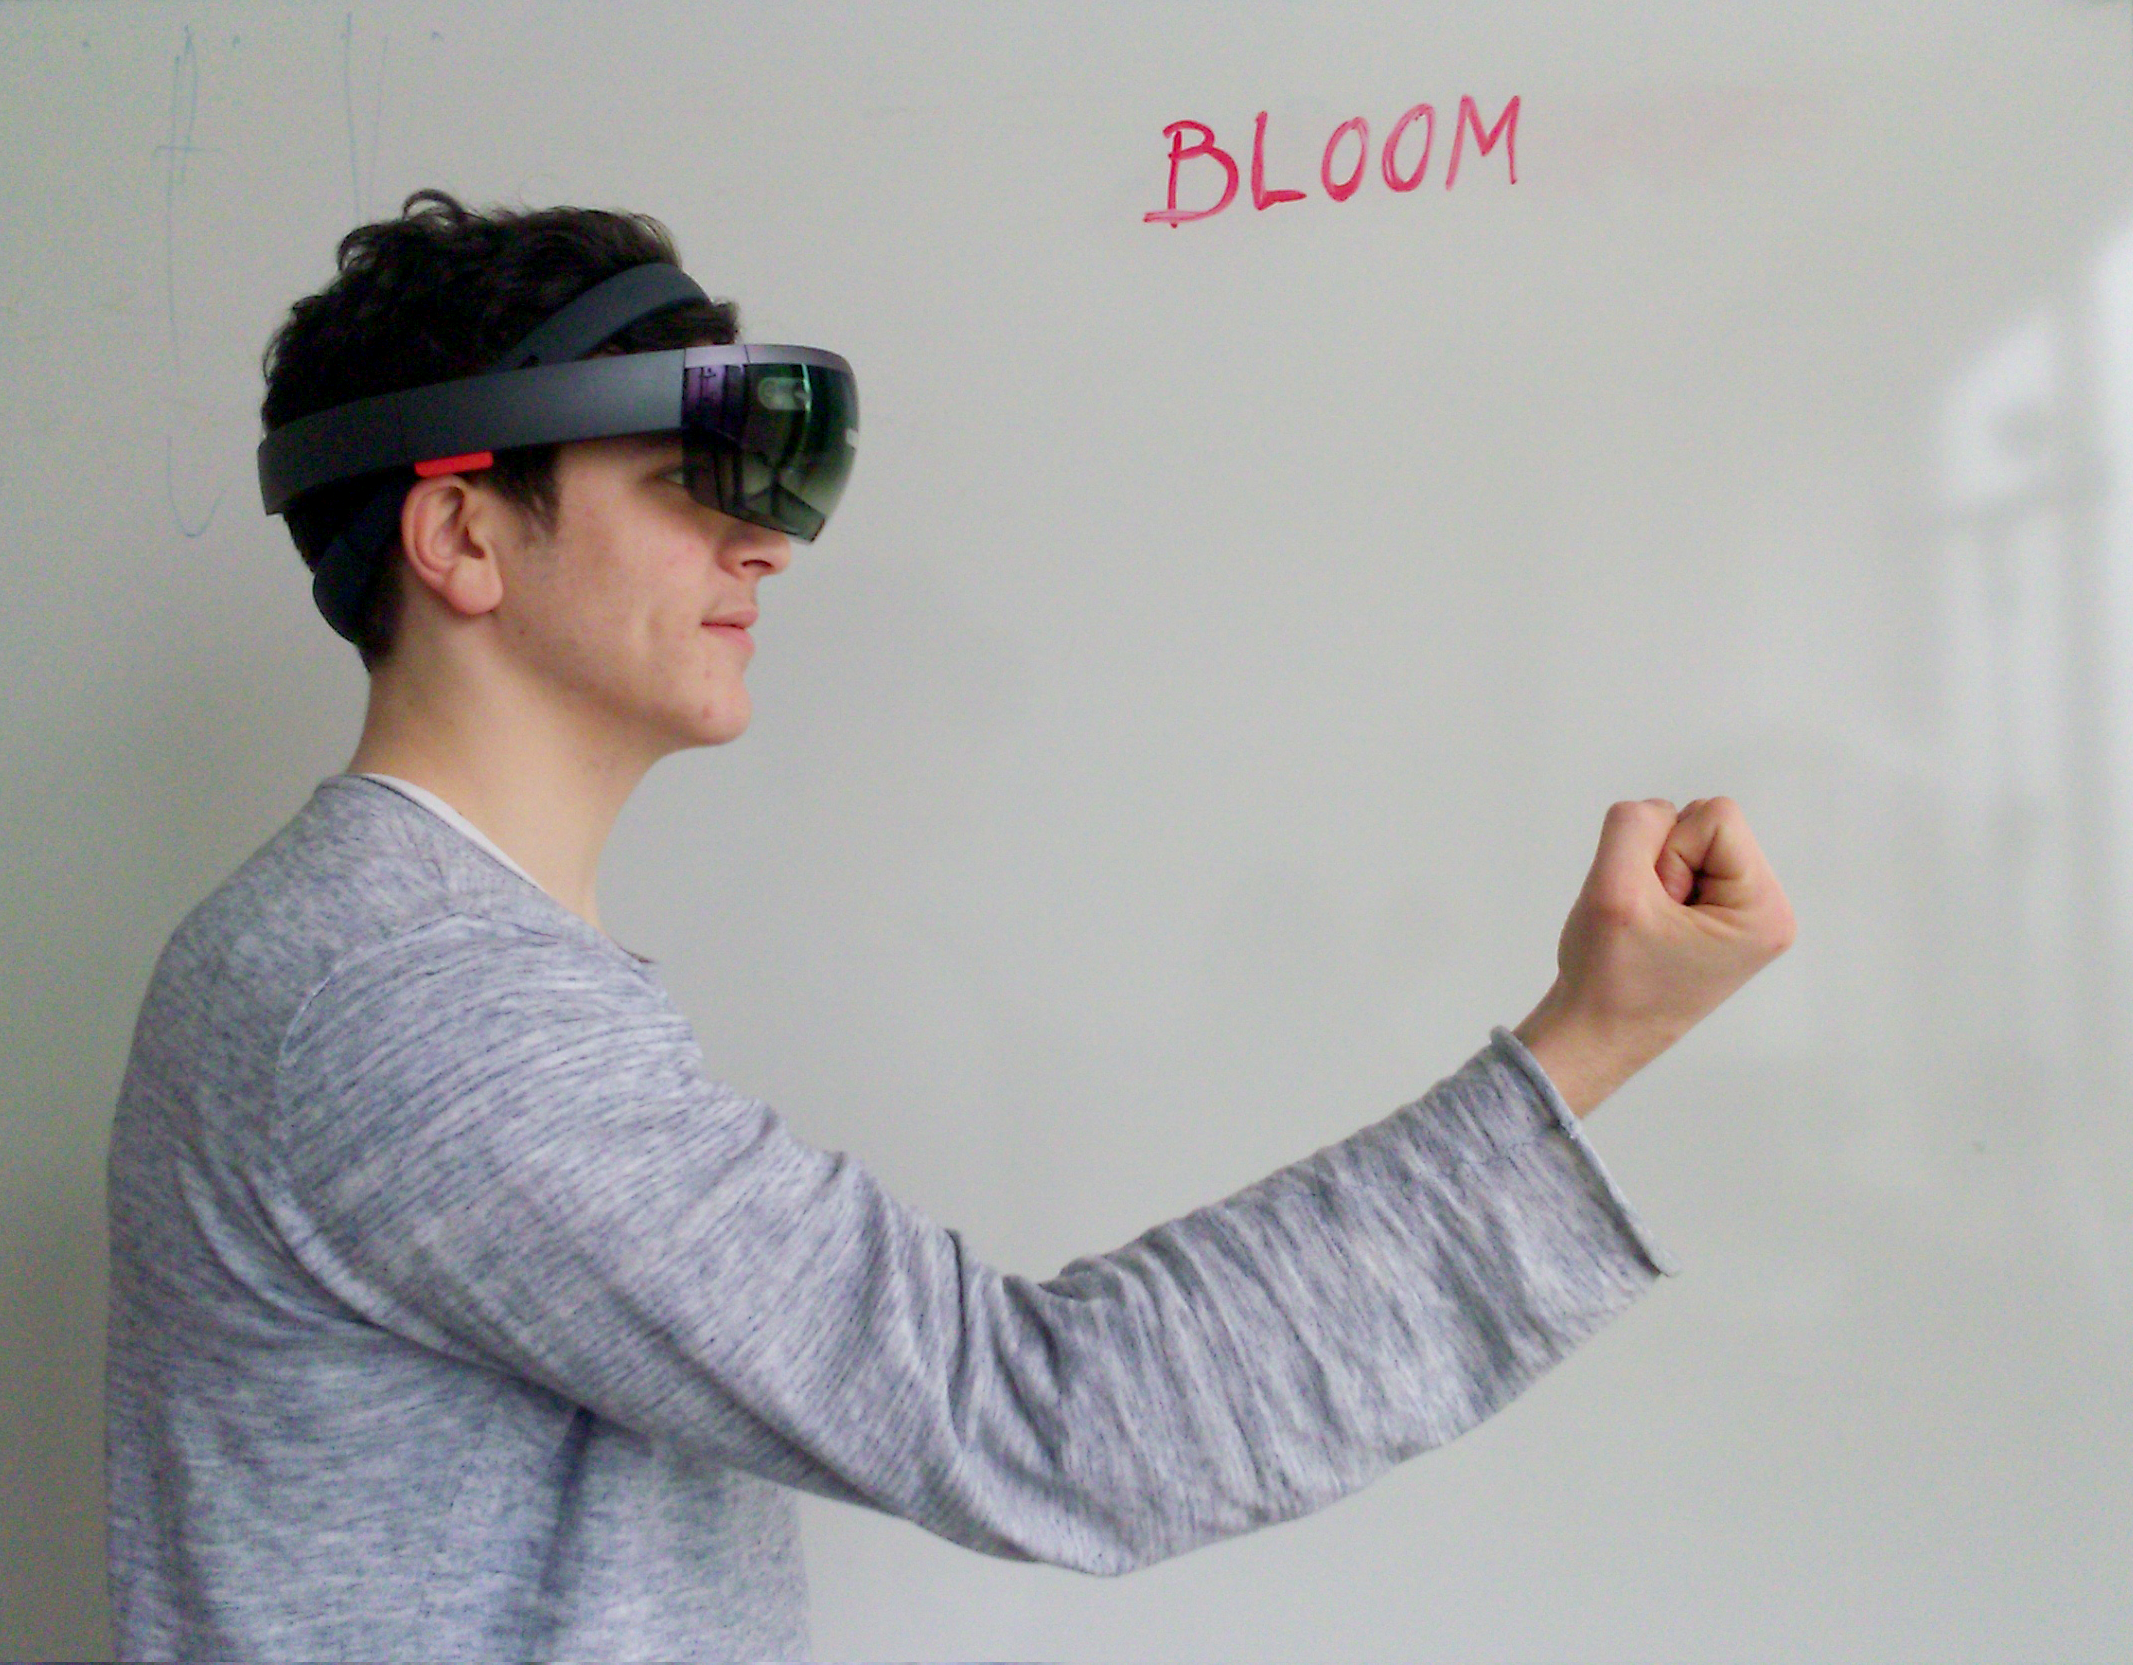
\includegraphics[width=.5\textwidth]{figuren/bloom1} &
		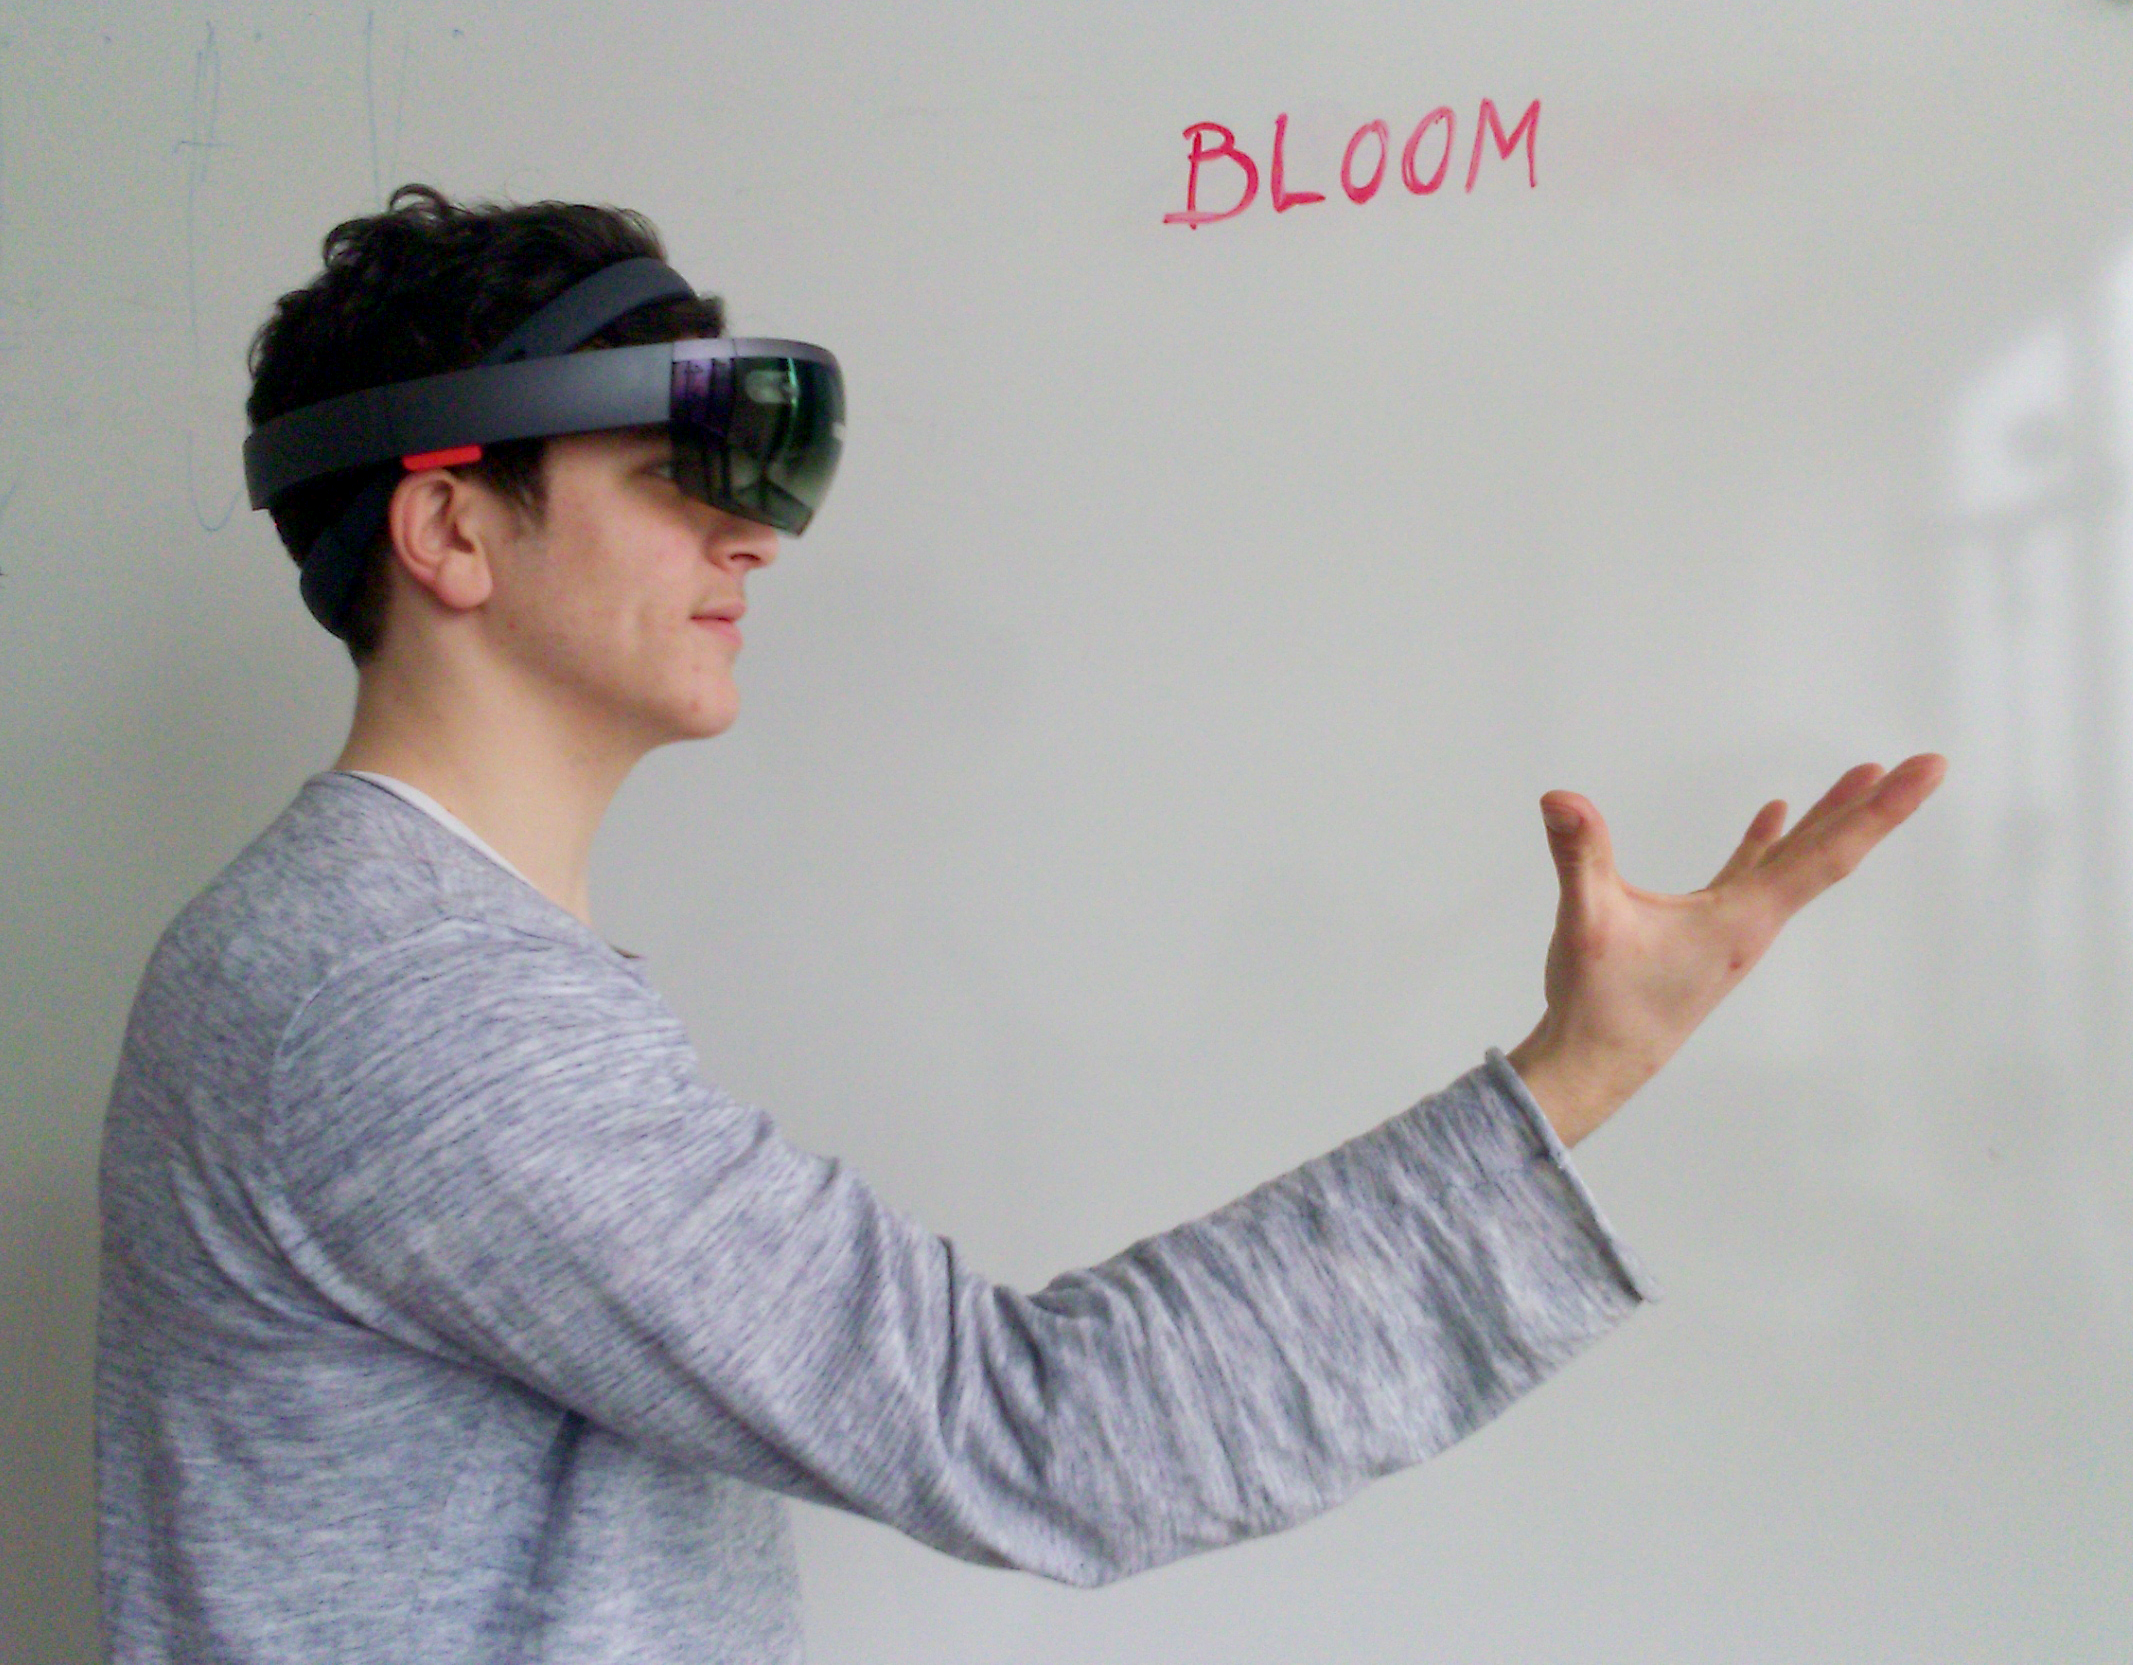
\includegraphics[width=.5\textwidth]{figuren/bloom2} \\
		(a) & (b)
	\end{tabular}
	\caption{
		\textit{Prepare Bloom Gesture (Fist)} (a), \textit{Perform Bloom Gesture} (b). Bildquelle: Eigenes Werk.
	}
	\label{fig:gesture_bloom}
\end{figure}
Die \textbf{Air-Tap}-Geste ist das Gegenstück zum klassischen Klick mit einer Maus am Computer. In Verbindung mit der \textit{Gaze}-Geste des Kopfes können somit Hologramme ausgewählt und Aktionen ausgelöst werden.\\\\Die Geste setzt sich aus einer schnellen Abfolge der \textbf{Tap-And-Hold}-Geste sowie der \textbf{Hold-And-Release}-Geste zusammen. Mit diesen lassen sich auch bekannte Manöver wie die \textit{Drag-And-Drop}-Interaktion am Computer imitieren. Beispielsweise kann man Hologramme in allen Freiheitsgraden bewegen, Bildschirminhalte verschieben (Scrollen) und andere Regler-Interaktionen, wie \textit{Zoomen} bedienen. Abbildung \ref{fig:scroll} zeigt, wie die Kombination aus diesen Gesten zusammen mit einer Translation der Hand auf der X-Achse und Y-Achse zum Scrollen verwendet werden kann.
\begin{figure}[H]
	\centering\small
	\setlength{\tabcolsep}{0mm}% alle Spaltenränder auf 0mm
	\begin{tabular}{c c} % mittlerer Abstand = 12mm
	  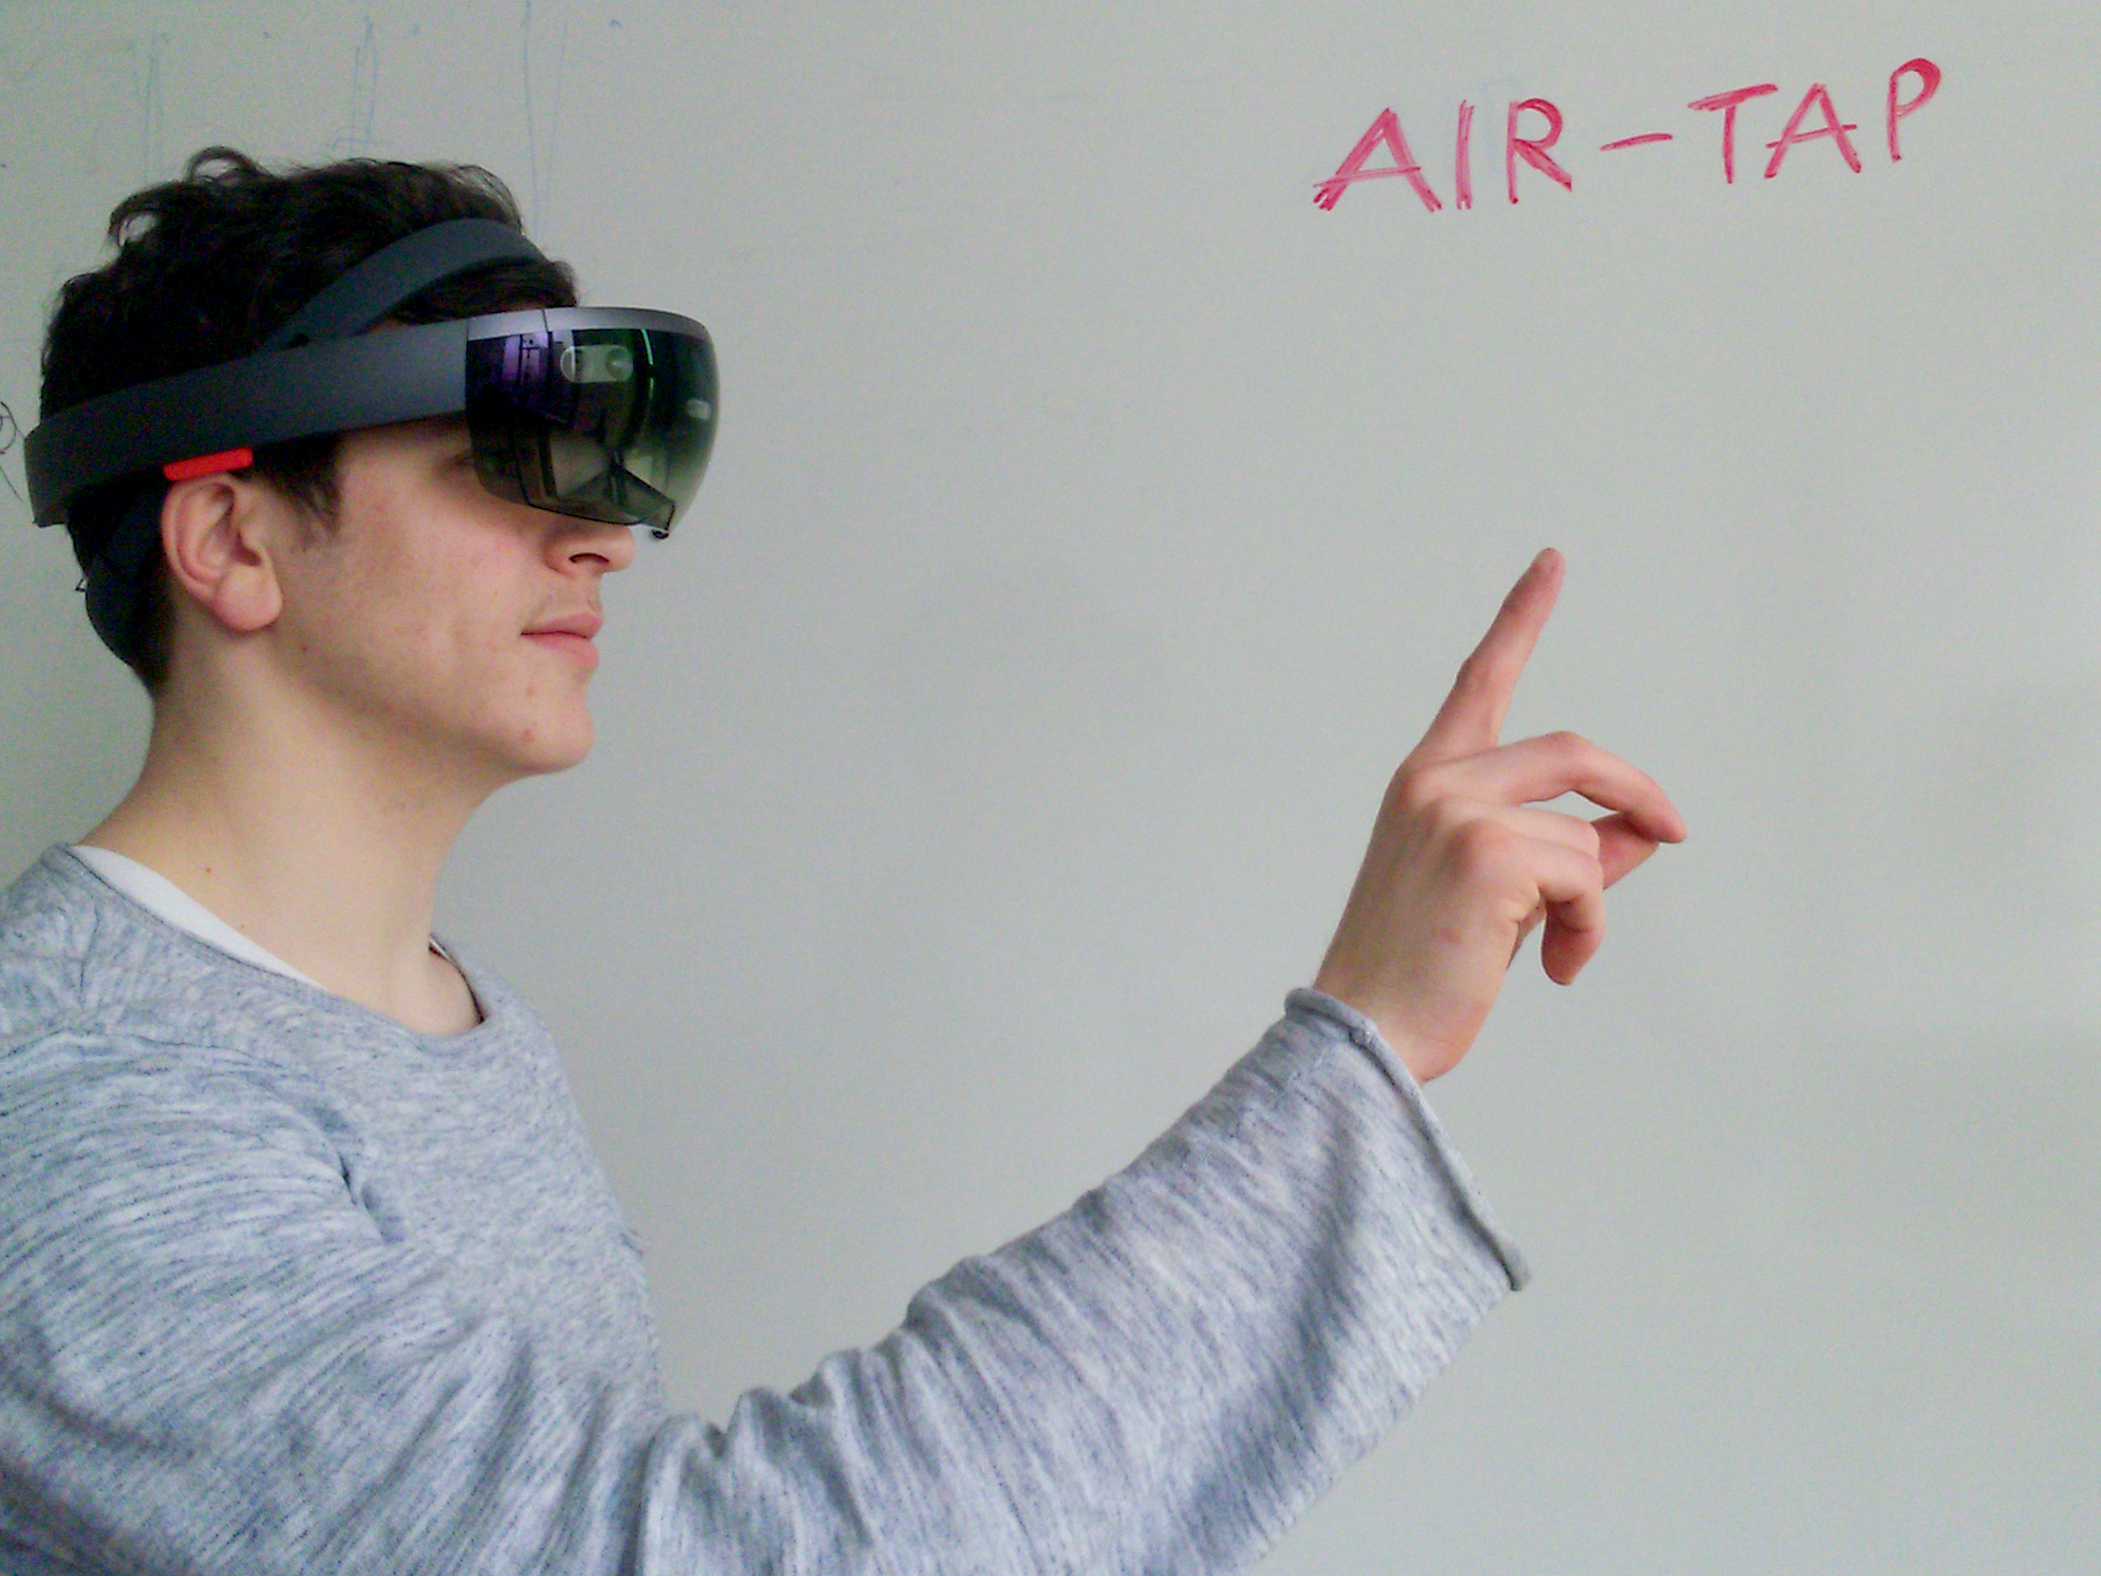
\includegraphics[width=.45\textwidth]{figuren/air_tap1} &
	  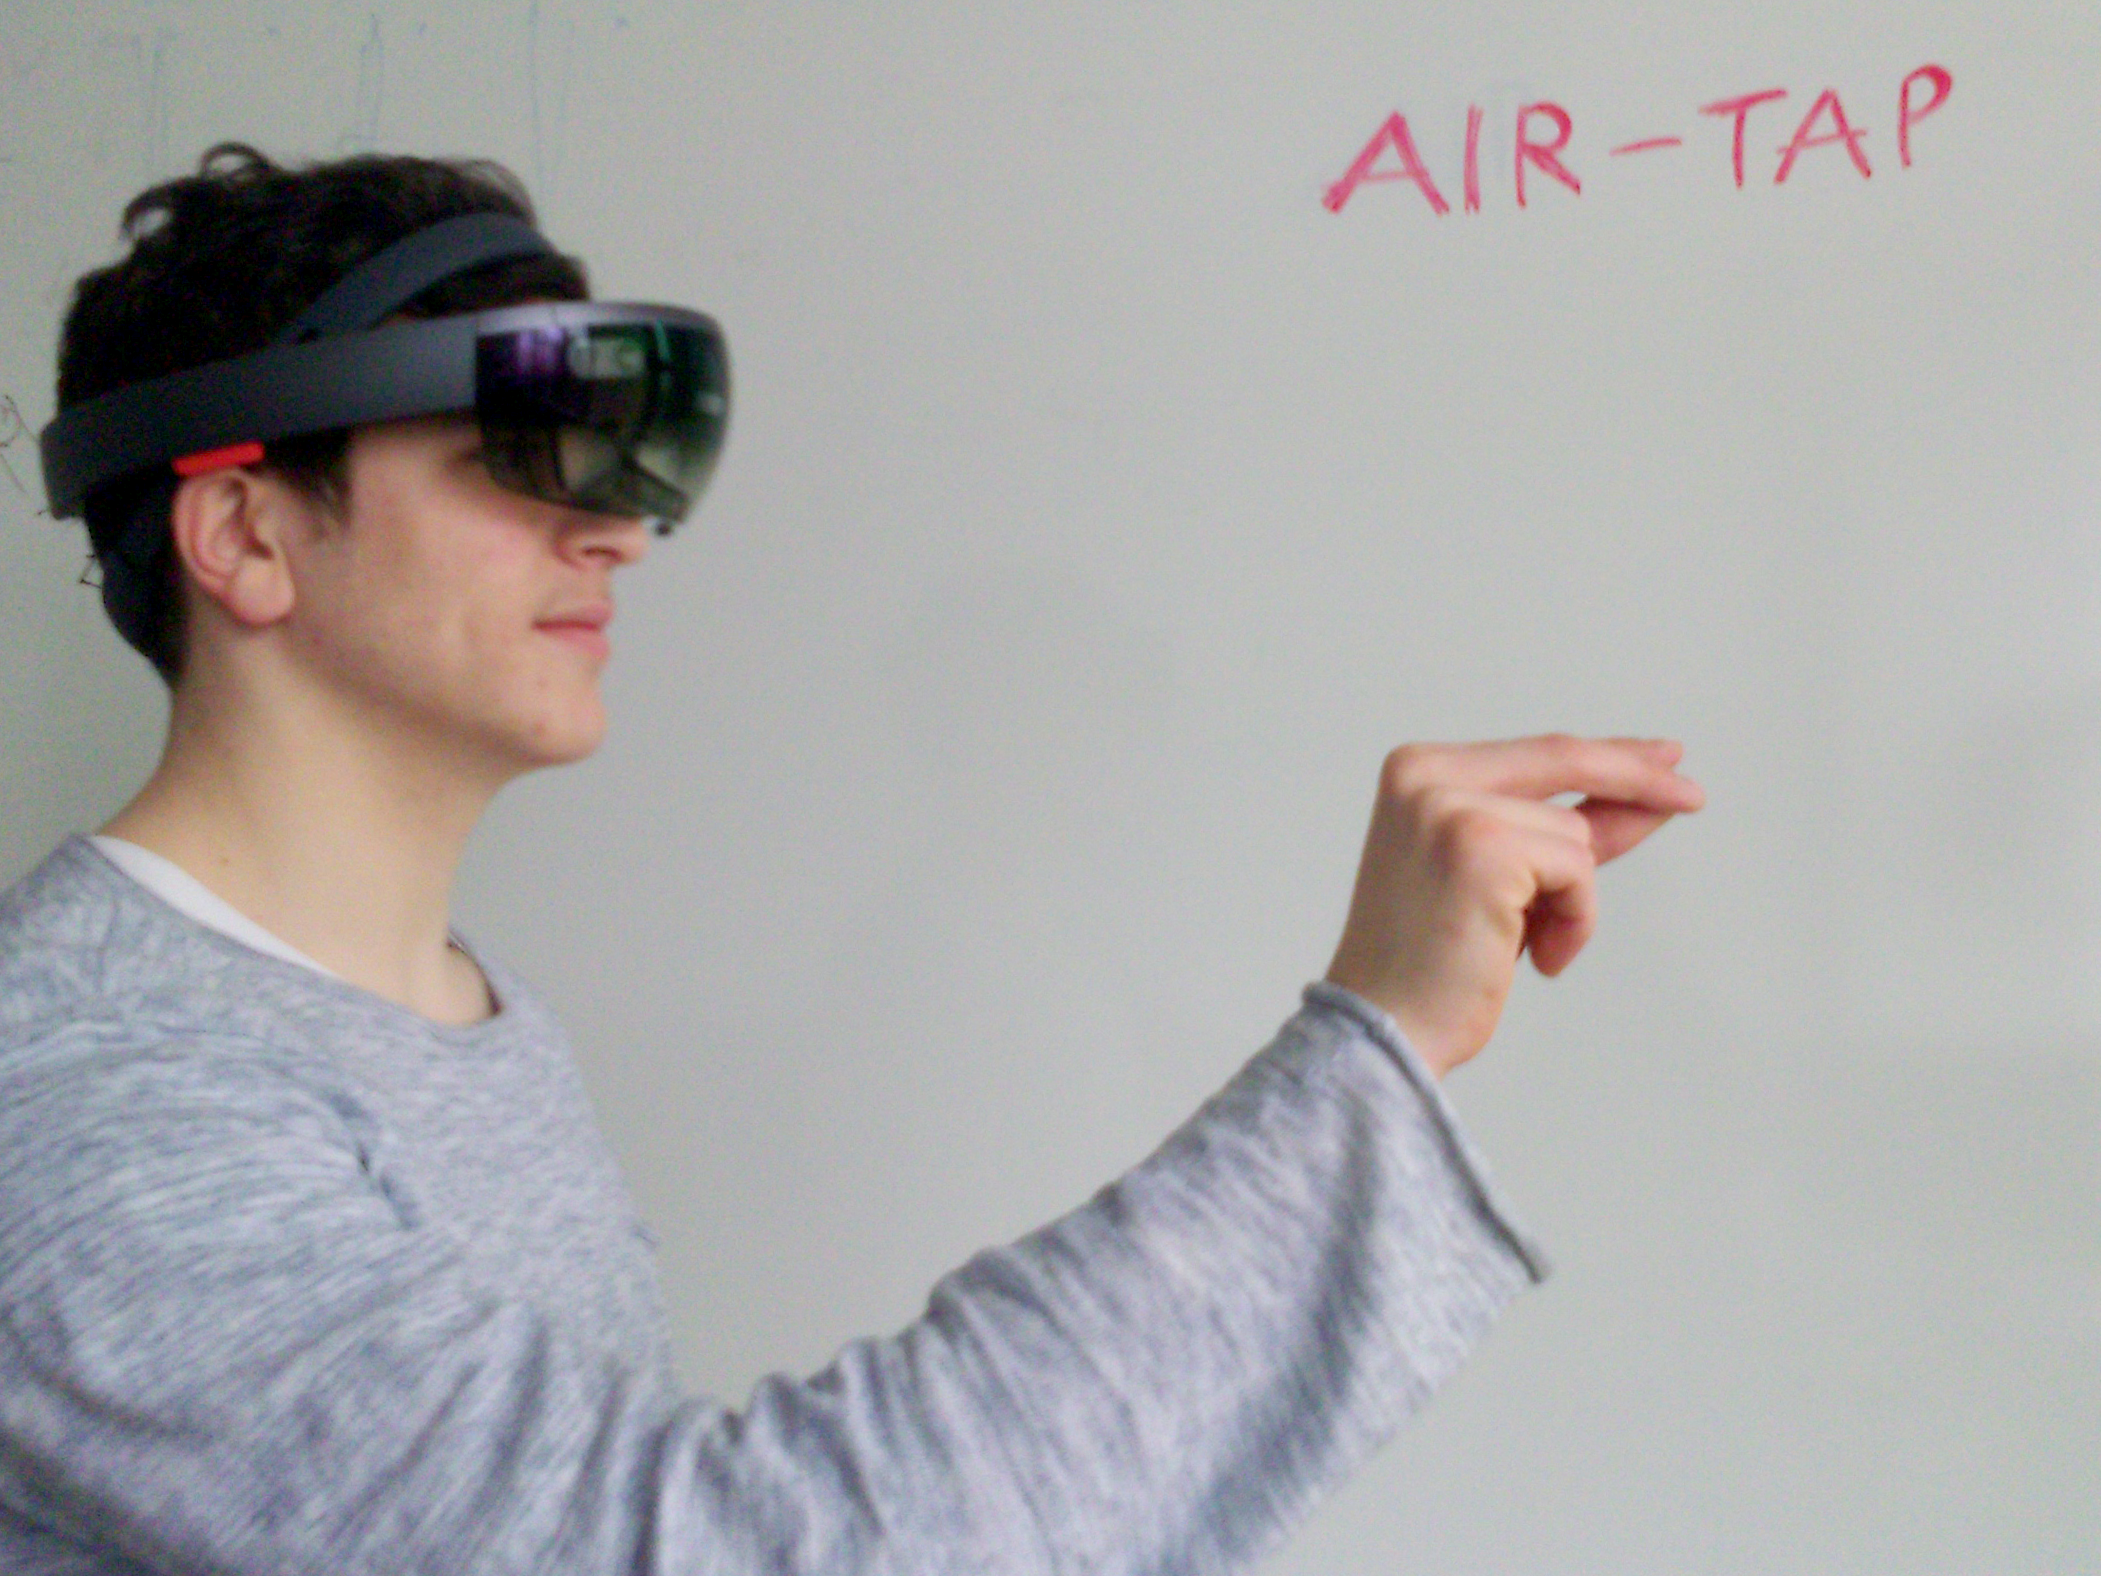
\includegraphics[width=.45\textwidth]{figuren/air_tap2} \\
	  (a) & (b) \\
	  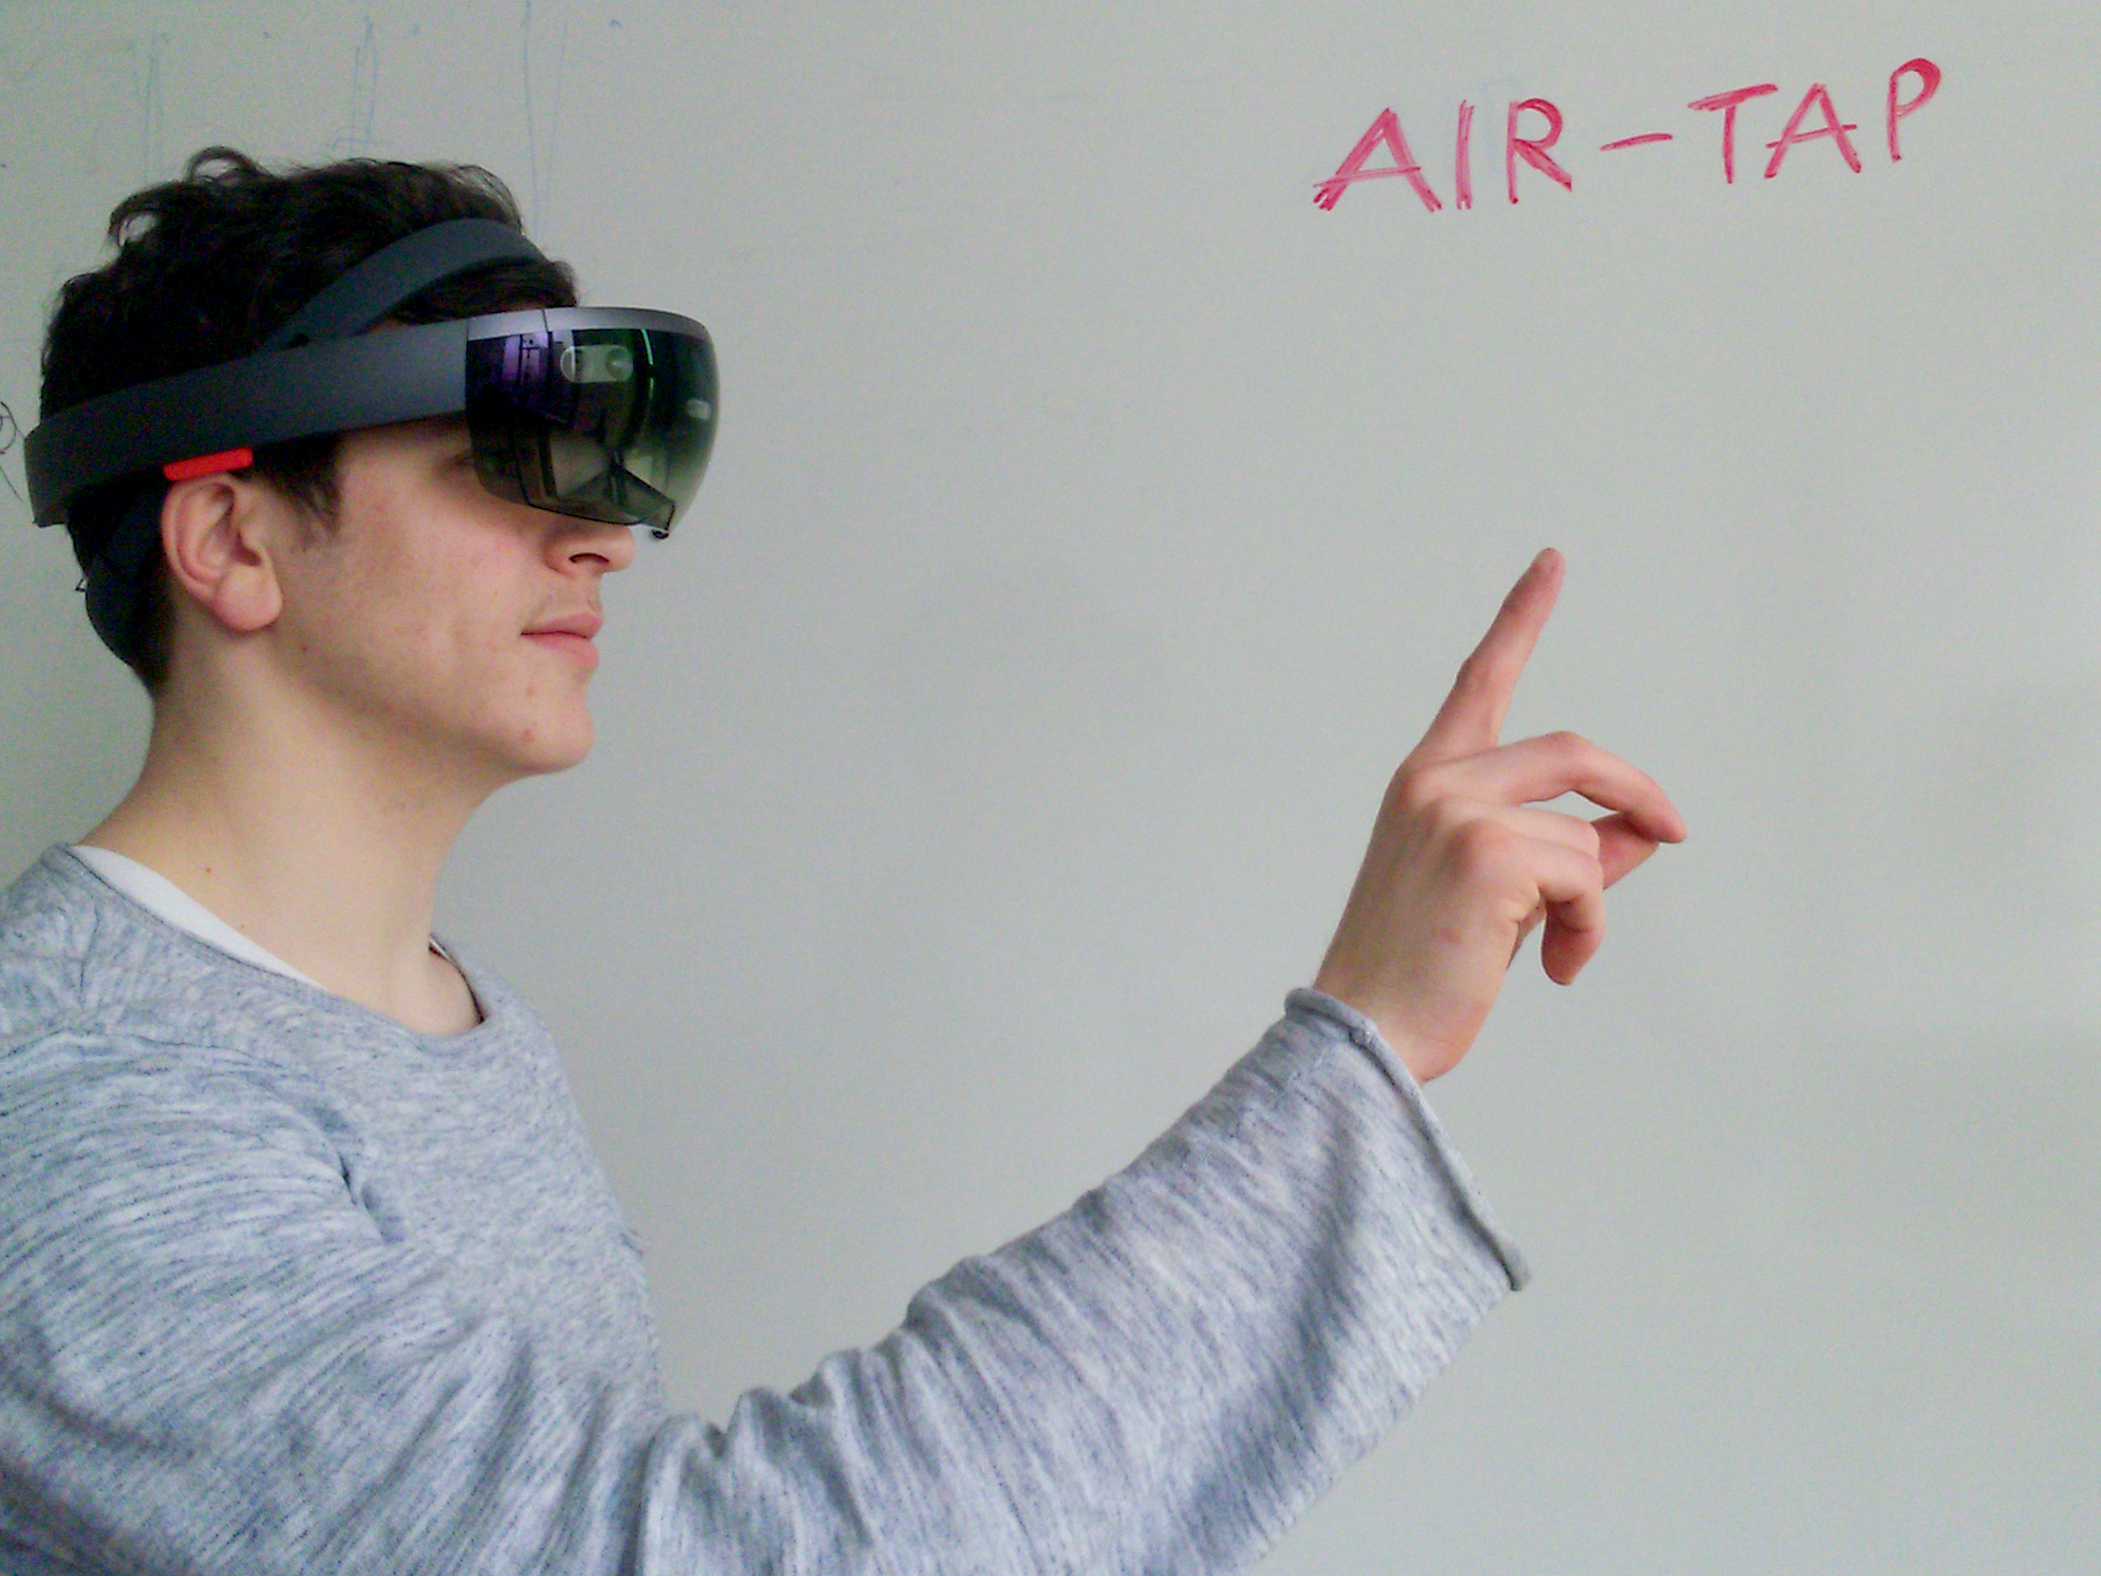
\includegraphics[width=.45\textwidth]{figuren/air_tap1} \\
	  (c)
	\end{tabular}
	%
	\caption{Die \textit{Air-Tap}-Geste. Initiiert mit der \textit{Gesture-Ready}-Geste (a), ausgeführt mit dem \textit{Tap} selbst (b) und Endposition erneute \textit{Gesture-Ready}-Geste (c). Bildquelle: Eigenes Werk.
	}
	\label{fig:gesture_air_tap}
\end{figure}
\begin{figure}[H]
	\centering
	\includegraphics[width=1.0\textwidth]{figuren/scroll}
	\caption{\textit{Scroll}-Geste in X- und Z-Richtung (\textit{Tap-And-Hold + Translation}). Bildquelle: Eigenes Werk.}
	\label{fig:scroll}
\end{figure}
\paragraph*{Voice-Commands} Die Spracherkennung der \textit{HoloLens} ist eine Interaktionsform zusätzlich zur Gesteninteraktion. In Menüs der \textit{HoloLens} sind alle interaktiven Schaltflächen auch mit Sprachkommandos aktivierbar. Dies trägt zur Barrierefreiheit bei und ist bei einer Spracherkennung mit einer Wort-zu-Fehlerrate von 5,9 Prozent durchaus als ein verlässliches Werkzeug anzusehen.\footnote{ Vgl. Xiong / Droppo / Huang / et al, o.S., 2016.}
\begin{figure}[H]
	\centering
	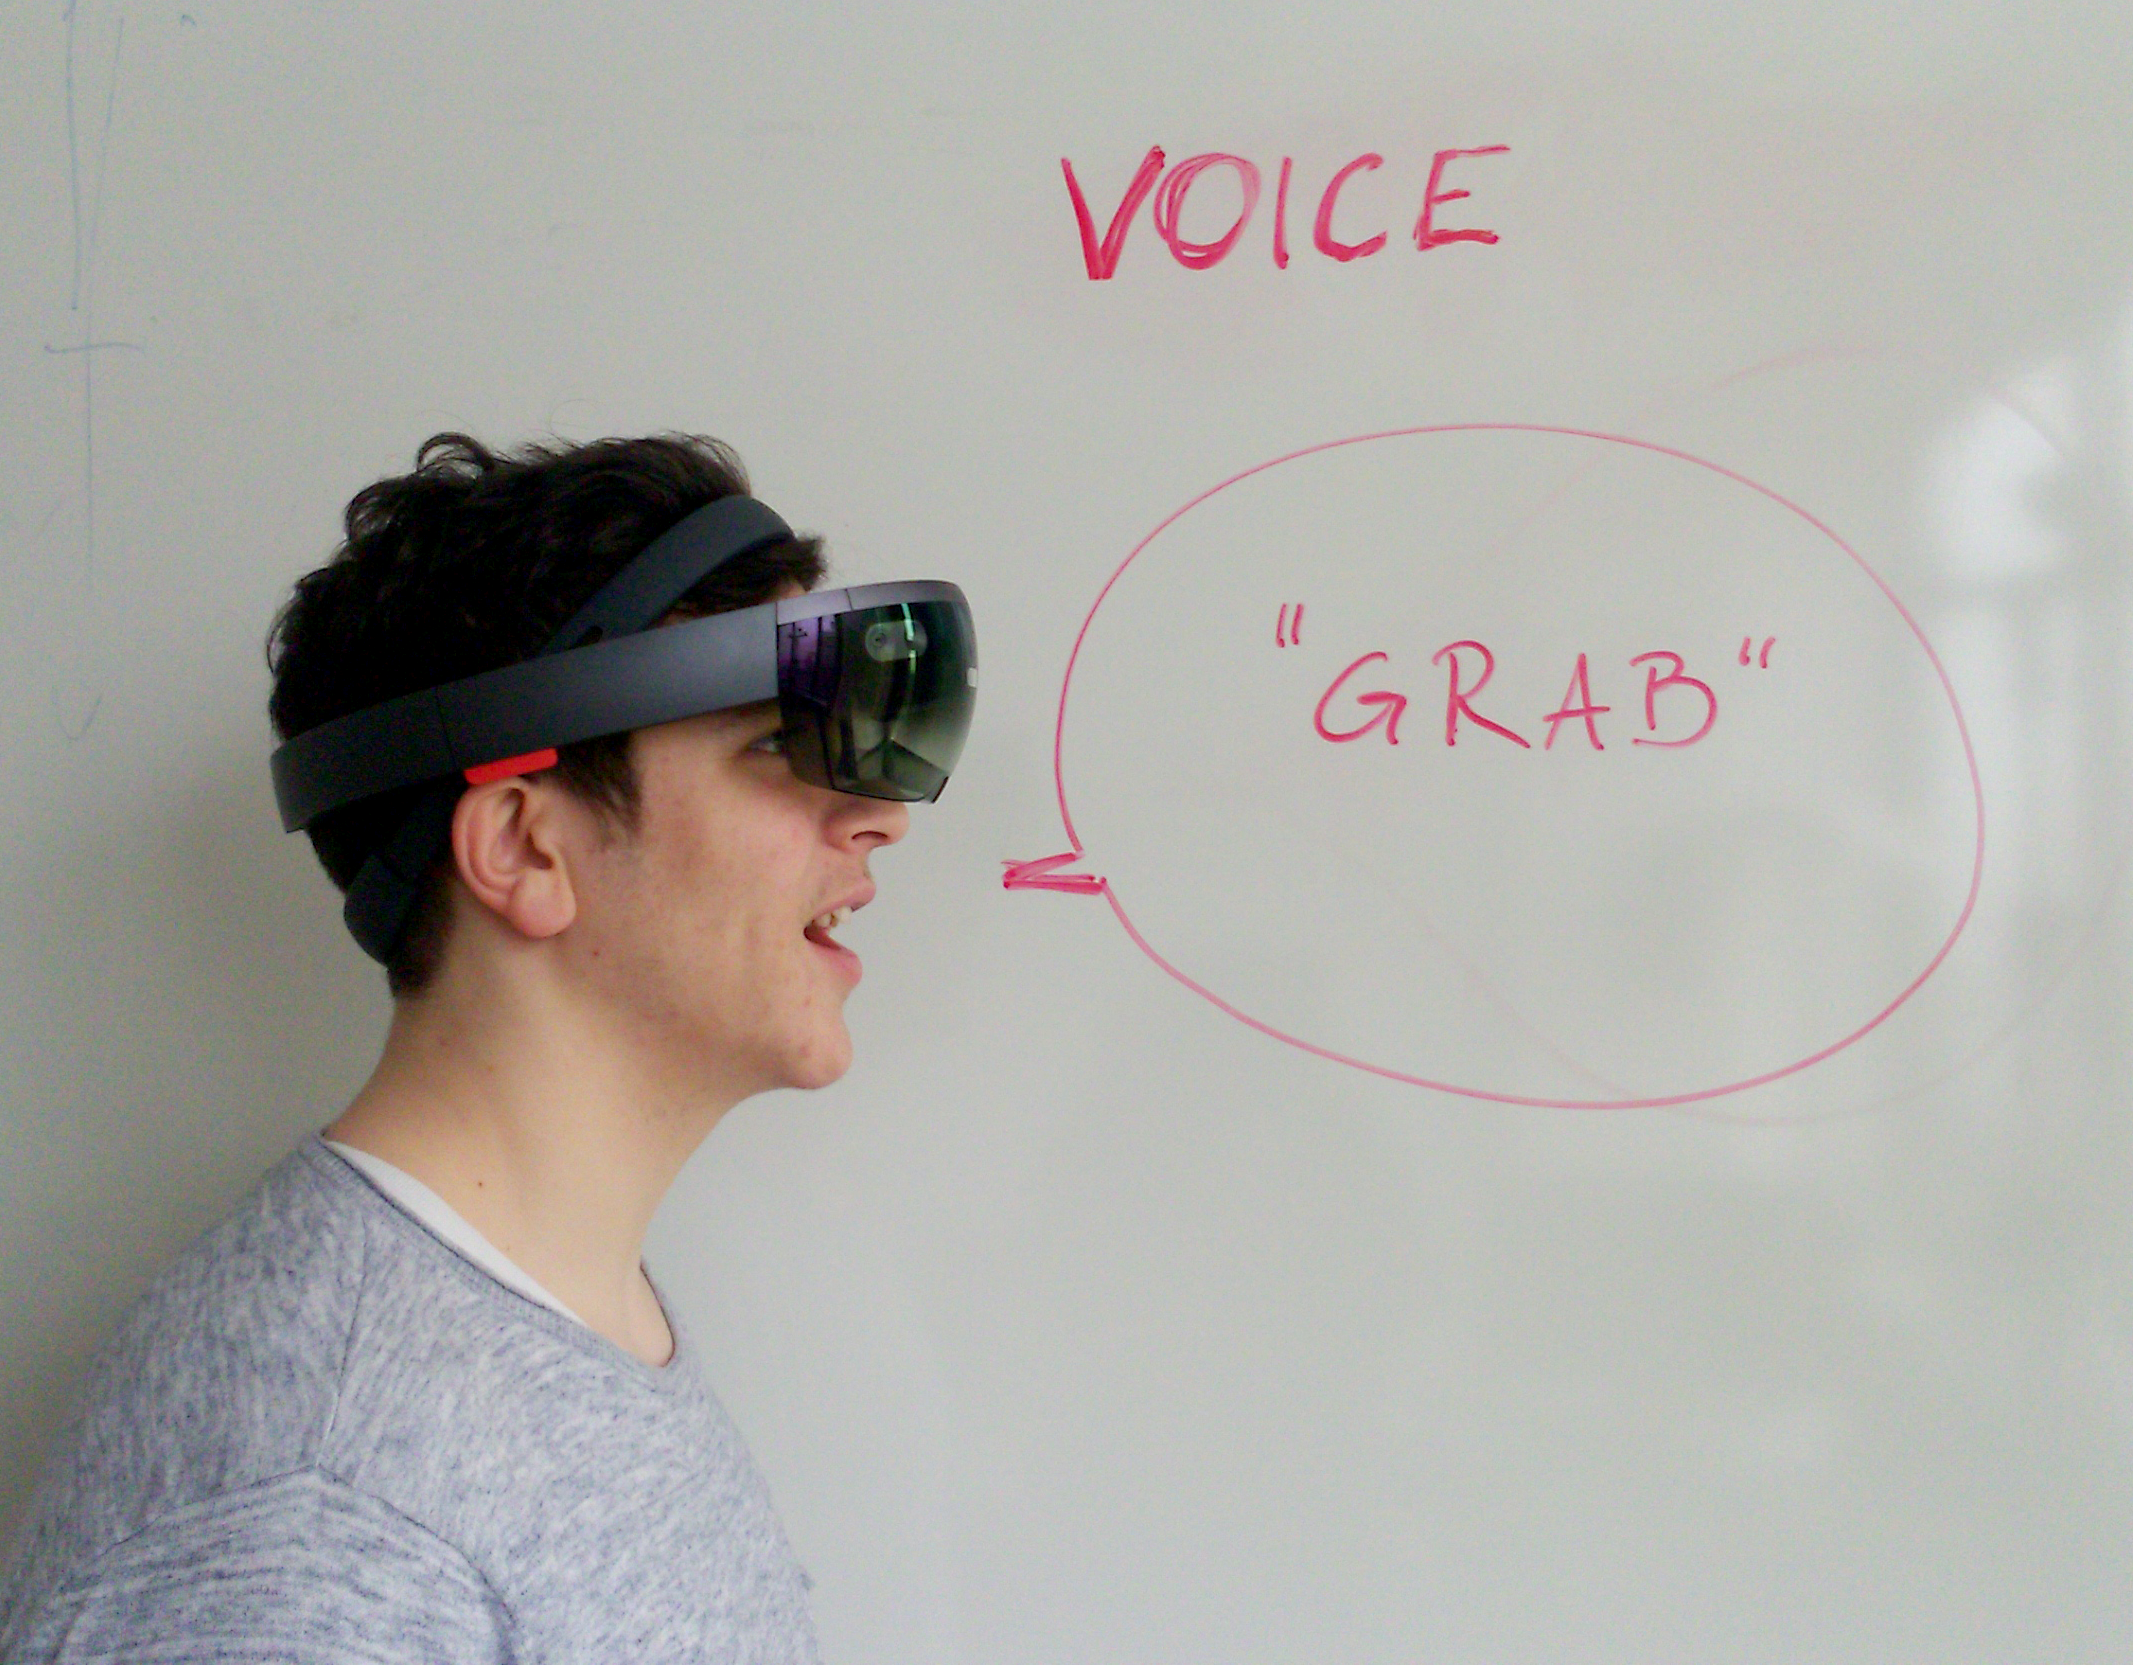
\includegraphics[width=1.0\textwidth]{figuren/voice}
	\caption{\textit{Voice-Command}: Am Beispiel \frqq Grab\flqq. Bildquelle: Eigenes Werk.}
	\label{fig:voice_command}
\end{figure}
Die Gesten- und Sprachinteraktion sind den HCI-Kriterien der ISO 9241-110\footnote{DIN 9241-110, Hrsg., o.S., 2008.} für Soft- und Hardwaresysteme nachempfunden. Sie tragen abgekürzt den Namen \frqq ASSEFIL\flqq-Kriterien:\begin{enumerate}
	\item Aufgabenangemessenheit:\\\frqq Ein Dialog ist aufgabenangemessen, wenn er den Benutzer unterstützt, seine Arbeitsaufgabe effektiv und effizient zu erledigen.\flqq
	\item Selbstbeschreibungsfähigkeit:\\\frqq Wenn eine Eingabe verlangt wird, sollte das Dialogsystem dem Benutzer Informationen über die zu erwartete Eingabe geben.\flqq
	\item Steuerbarkeit:\\\frqq Ein Dialog steuerbar, wenn der Benutzer in der Lage ist, den Dialogablauf zu starten sowie seine Richtung und Geschwindigkeit zu beeinflussen, bis das Ziel erreicht ist\flqq
	\item Erwartungskonformität:\\\frqq Ein Dialog ist erwartungskonform, wenn er konsistent ist und den Merkmalen des Benutzers entspricht, zum Beispiel seinen Kenntnissen aus dem Arbeitsgebiet und seinen Erfahrungen sowie den allgemein anerkannten Konventionen.\flqq
	\item Fehlertoleranz:\\\frqq Ein Dialog ist fehlertolerant, wenn das beabsichtigte Arbeitsergebnis trotz erkennbarer Fehleingaben entweder mit keinem oder mit minimalem Korrekturaufwand seitens des Benutzers erreicht werden kann.\flqq
	\item Individualisierbarkeit:\\\frqq Ein Dialog ist individualisierbar, wenn Benutzer die Mensch-System-Interaktion und die Darstellung von Informationen ändern können, um dise an ihre individuellen Fähigkeiten und Bedürfnisse anzupassen.\flqq
	\item Lernförderlichkeit:\\\frqq Ein Dialog ist lernförderlich, wenn er den Benutzer beim Erlernen der Nutzung des interaktiven Systems unterstützt und anleitet.\flqq
\end{enumerate}
Im nächsten Kapitel wird, mit den im Kapitel~\ref{chapter:Grundlagen} vorgestellten Technologien und Interaktionen, das Konzept für die prototypische Implementierung vorgestellt.
\newpage
\chapter{Konzeption}\label{chapter:Konzeption}
In diesem Kapitel werden zunächst Kriterien definiert, die das Anwendungssystem im Rahmen dieser Abschlussarbeit erfüllen soll. Hierbei wird auf die Zielsetzung geachtet und Anwendungsfälle, sogenannte \textit{Use Cases}, entwickelt, die ein Anwender mit der prototypischen Implementierung bestreiten können soll. Des Weiteren wird der Systementwurf genauer betrachtet. Dazu zählen insbesondere das Zusammenwirken der einzelnen Komponenten, welche Schichten abstrahiert werden und wie der Informationsfluss in den einzelnen Komponenten ist.
\section{Spezifikation}
Bei der zu entwickelnden Software handelt es sich um ein \textit{User Interface}, dass den Anwender dazu befähigt einen Roboter mit Hilfe der Gesten- und Stimmenerkennung der \textit{Microsoft HoloLens} über das Netzwerk fernzusteuern. Für die Verwendung wird ein Roboter, der eine Netzwerkschnittstelle besitzt, eine \textit{Microsoft HoloLens}, die die Gestensteuerung erkennt und dem Anwender Hilfestellung in grafischer Form bietet sowie eine aktive, kabellose Netzwerkverbindung benötigt. Abbildung~\ref{fig:pipeline} beschreibt schematisch den Informationsfluss in der Anwendung.
\begin{figure}[H]
	\centering
	\includegraphics[width=1.0\textwidth]{figuren/Pipeline}
	\caption{Informationsfluss in der Applikation \textit{EV3ControllAR}. Bildquelle: Eigenes Werk.}
	\label{fig:pipeline}
\end{figure}
\subsection{Zielsetzung}
Das Ziel der Applikation ist es, zu erfassen, ob und inwieweit Gesten und Sprachkommandos eine natürliche Interaktionsform und Schnittstelle für die in Zukunft verschmelzenden Welten von Robotern und Menschen sind und ob Anwender diese beim Lösen kleiner Aufgaben als intuitiv empfinden.
\subsection{Anwendungsfall}\label{ssec:usecase}
Die funktionalen Anforderungen der Anwendung werden mit Hilfe von Anwendungsfällen ermittelt. Diese abstrahieren die Interaktion zwischen Benutzer und Anwendung und machen deutlich, was die Applikation aus Sicht des Benutzers leisten muss und inwiefern sie den Benutzer unterstützen kann. In Abbildung \ref{fig:useCaseDiagram} sieht man das Anwendungsfalldiagramm in der \textit{Unified Modelling Language}(UML) modelliert. Es zeigt die einzelnen Fälle der Applikation gebündelt in einem Diagramm. 
\begin{figure}[H]
	\centering
	\includegraphics[width=1.0\textwidth]{figuren/UseCaseDiagram}
	\caption{UML \textit{Use-Case}-Diagramm -- CommandRobot. Bildquelle: Eigenes Werk.}
	\label{fig:useCaseDiagram}
\end{figure}
Aus diesem wurden dann drei explizitere untergeordnete Anwendungsfälle aufgegliedert. Diese wurden nach dem Prinzip der \textit{User Story} entwickelt. Die \textit{User Story} beschreibt aus Sicht des Anwenders oder Kundens, was eine Software leisten soll und was der Anwender sich diesbezüglich wünscht.\footnote{ Vgl. Wells, o.S., 1999, [Accessed: 04.01.2017].}

\textbf{Anwendungsfall 1 -- MoveRobot -- Roboter bewegen}\\
\frqq Als Anwender möchte ich den Roboter auf seiner Schiene frei bewegen können; dabei ist es mir wichtig, dass ich die volle Kontrolle über Geschwindigkeit und Position des Roboters habe.\flqq
\begin{table}[H]
	\centering
	\begin{tabular}{|l|p{8cm}|}
		\hline
		\textbf{Name} & Roboter bewegen (MoveRobot) \\
		\hline
		\textbf{Ziel im Kontext} & Roboter bewegt sich von Position A zu Position B \\
		\hline
		\textbf{Akteure} & Anwender und Roboter \\
		\hline
		\textbf{Trigger} & Anwender verschiebt 3D-Objekt in Szene \\
		\hline
		\textbf{Essentielle Schritte} & Richtiges 3D-Objekt auswählen \newline Korrekte Geste zum Translatieren in X-Richtung ausführen \newline 3D-Objekt freigeben \\
		\hline
		\textbf{Mögliche Erweiterungen} & Freies Translatieren ohne 3D-Objekt \\
		\hline
	\end{tabular}
	\caption{Anwendungsfall 1 -- \frqq Roboter bewegen\flqq.}
	\label{tab:usecase1}
\end{table}
\textbf{Anwendungsfall 2 -- GrabObject -- Objekt aufnehmen}\\
\frqq Als Anwender möchte ich mit Hilfe des Roboters Gegenstände in Reichweite aufheben; dabei ist es mir wichtig, dass der Roboter die Gegenstände präzise aufnimmt und bei Bewegungen in seinen Greifern behält.\flqq
\begin{table}[H]
	\centering
	\begin{tabular}{|l|p{8cm}|}
		\hline
		\textbf{Name} & Mit Roboter Objekt greifen (GrabObject) \\
		\hline
		\textbf{Ziel im Kontext} & Greift ein Objekt mit Greifern \\
		\hline
		\textbf{Akteure} & Anwender und Roboter \\
		\hline
		\textbf{Trigger} & Anwender verschiebt 3D-Objekt in Szene \\
		\hline
		\textbf{Essentielle Schritte} & Richtiges 3D-Objekt auswählen \newline Korrekte Geste zum Translatieren in Z-Richtung ausführen \newline 3D-Objekt freigeben \\
		\hline
		\textbf{Mögliche Erweiterungen} & Freies Translatieren ohne 3D-Objekt \\
		\hline
	\end{tabular}
	\caption{Anwendungsfall 2 -- \frqq Objekt aufnehmen\flqq.}
	\label{tab:usecase2}
\end{table}
\textbf{Anwendungsfall 3 -- PlaceObject -- Objekt platzieren}\\
\frqq Als Anwender möchte mit Hilfe des Roboters einen aufgenommenen Gegenstand an einer beliebigen Position ablegen; dabei ist es mir wichtig, dass der Roboter die Gegenstände präzise, druch öffnen der Greifer, absetzt und sie zur Aufnahme neuer Objekte offen hält.\flqq
\begin{table}[H]
	\centering
	\begin{tabular}{|l|p{8cm}|}
		\hline
		\textbf{Name} & Mit Roboter Objekt platzieren (PlaceObject)  \\
		\hline
		\textbf{Ziel im Kontext} & Roboterarm bewegt sich gen Boden und öffnet Greifer \\
		\hline
		\textbf{Akteure} & Anwender und Roboter \\
		\hline
		\textbf{Trigger} & Anwender aktiviert Sprachbefehl mit Stimme \\
		\hline
		\textbf{Essentielle Schritte} & Richtigen Sprachbefehl \newline Korrekte Abfolge von Worten aussprechen \newline \\
		\hline
		\textbf{Mögliche Erweiterungen} & Translatieren eines 3D-Objekts in Z-Richtung als Trigger \\
		\hline
	\end{tabular}
	\caption{Anwendungsfall 3 -- \frqq Objekt platzieren\flqq.}
	\label{tab:usecase3}
\end{table}
\textbf{Anwendungsfall 4 -- EmergencyStop -- Notstopp}\\
\frqq Als Anwender möchte ich den Roboter immer und mit sofortiger Wirkung anhalten können; dabei ist es mir wichtig, dass alle Motoren anhalten, Greifer und Arm sollten in ihrer bisherigen Position verweilen und der Bewegungsapparat zum Stehen kommen.\flqq
\begin{table}[H]
	\centering
	\begin{tabular}{|l|p{8cm}|}
		\hline
		\textbf{Name} & Notstopp (Stop)  \\
		\hline
		\textbf{Ziel im Kontext} & Roboter stoppt sofort alle Motoren \\
		\hline
		\textbf{Akteure} & Anwender und Roboter \\
		\hline
		\textbf{Trigger} & Anwender aktiviert Sprachbefehl mit Stimme \\
		\hline
		\textbf{Essentielle Schritte} & Richtigen Sprachbefehl oder \textit{Bloom}-Geste\\
		\hline
		\textbf{Mögliche Erweiterungen} & Notknopf am Körper. \\
		\hline
	\end{tabular}
	\caption{Anwendungsfall 4 -- \frqq Notstopp\flqq.}
	\label{tab:usecase4}
\end{table}
\subsection{Muss-Kriterien}
Die Anwendungsfälle resultieren in folgenden Funktionen, die dem Nutzer in der Applikation sofort und immer zur Verfügung stehen müssen:

\begin{itemize}
	\item Gestenerkennung
	\item Kenntlichmachung, wenn Gesten angewendet werden können (Gesture-Ready)
	\item Unterscheidung von Gesten:
	\begin{itemize}
		\item Tap-Geste um 3D-Objekte auszuwählen
		\item Tap-And-Hold-Geste um 3D-Objekte als \textit{draggable} auszuwählen
		\item Translatieren von 3D-Objekten in X-Richtung
	\end{itemize}
	\item Symbolisierung der oben genannten Gesten mit Icons
	\item Interface zur Übersicht des Roboters und dessen Funktionen
	\item \textbf{Notstopp}, sofortiger Stopp aller Motoren
\end{itemize}
\subsection{Kann-Kriterien}
Kann-Kriterien bezeichnen die Kriterien, deren Umsetzung sehr erstrebenswert wären. Allerdings sprengen sie im Kontext von Bachelorarbeiten meistens den zeitlichen Rahmen.

\begin{itemize}
	\item Roboter kann sich in allen Freiheitsgraden bewegen
	\item Dem Benutzer stehen weitere Gesten zur Verfügung
	\begin{itemize}
		\item Rotationsgesten, ähnlich dem Drehen eines Drehreglers
		\item \textit{Eyetracking} zur schnelleren Lokalisierung von Punkten im Raum
		\item Verbindung mit zusätzlichem \textit{Wearables} für mehr Interaktionsspielraum und Nutzung von bereits bekannten Gesten, wie \textit{Touch} oder Tasten
	\end{itemize}
	\item Roboter bewegt sich frei im Raum, nicht auf Schiene
	\begin{itemize}
		\item Wegfindung
		\item Visualisierung des Pfades im HMD
		\item Setzen von Wegpunkten aus dem HMD heraus
		\item Erweiterte Routenoptionen
	\end{itemize}
	\item Weitere Anwendungsszenarien
\end{itemize}
\subsection{Abgrenzungskriterien}
Die Abgrenzungskriterien stellen Kriterien dar, welche aufzeigen, was das System nicht leisten soll, um es klar von anderen Systemen abzugrenzen.

Die Grenzen dieses Produkts belaufen sich im Allgemeinen darauf, dass die Applikation nur ein Prototyp ist, welcher die Machbarkeit überprüfen und das Gefühl der kontrollierten Steuerung übertragen soll. Sie belaufen sich des Weiteren auf folgende Punkte:
\begin{itemize}
	\item Verwendbarkeit unter echten Produktionsbedingungen
	\item Verwendung in Echtzeit
	\item Synchronität von Gesten und Bewegung des Roboters
	\item Sicherheit
	\item Skalierbarkeit
	\item Simultane Verwendbarkeit eines Roboters durch mehrere Anwender
	\item Generische Nutzung von Maschinen
\end{itemize}
\subsection{Nicht funktionale Kriterien}
Was \frqq nicht funktionale Kriterien\flqq\ sind, ist nicht einheitlich definiert, jedoch ist allen Definitionen gemein, dass \frqq nicht funktionale Kriterien\flqq\ mit Metriken beschreiben, wie gut/zuverlässig ein System funktionieren soll.\footnote{ Vgl. Rupp, S. 268f, 2014.}\\
In der vorliegenden Arbeit wird besonderer Wert darauf gelegt, dass die Applikation \textit{EV3ControllAR} folgende Kriterien erfüllt:
\paragraph*{Aussehen}
Ebenso ist es für die Anwendung der vorliegenden Arbeit wichtig, dass sowohl das \textit{Interface} Design als auch die Code-Struktur sauber, modern, übersichtlich und gut strukturiert ist. Dazu zählt auch die Wartbarkeit des Codes durch Lesbarkeit und fundierte Dokumentation.
\paragraph*{Benutzbarkeit}
In der vorliegenden Arbeit wird ebenfalls hoher Wert darauf gelegt, dass die Anwendung eine leichte Verständlichkeit bietet, sodass sich dem Anwender die Benutzbarkeit erschließt und durch er visuelle Signale gestützt wird. Außerdem sollte sie, soweit dies bei innovativen Interaktionsformen möglich ist, durch sich wiederholende, bekannte und bereits erlernte Muster und Metaphern gefördert werden. Hinzu kommt die Reaktionszeit des Roboters, die unter einer Sekunde liegen soll.
\subsection{Anwendungsumgebung}
In diesem Bereich wird erläutert, in welcher Anwendungsumgebung die Applikation ihren Sinn findet und unter welchen Bedingungen sie läuft. Zunächst sei dargelegt, dass die prototypische Version nur unter Laborbedingungen arbeitet, wohingegen das Konzept sowohl für Werkshallen, als auch menschenfeindliche Arbeitsumgebungen,
beispielsweise die Atmosphäre eines anderen Planeten, verseuchte oder unwegsame
Gebiete der Erde, das All oder auch alle Umgebungen, bei denen ein ferngesteuerter Roboter einen Sinn ergibt, entwickelt wurde.

Die Anwendung an sich kann dank \textit{Unity} für verschiedene Betriebssysteme kompiliert werden. Allerdings macht es nur Sinn, sie als Windows-App für die \textit{HoloLens} zu \textit{builden}, da die Schnittstellen des \textit{HoloToolkit} nur die Datenbrille von Windows ansprechen. Für die Ausführung unter Laborbedingungen benötigt man folgende Hardware:
\begin{itemize}
	\item \textit{Microsoft HoloLens}
	\item \textit{Lego Mindstorms EV3} mit \textit{WiFi USB-Dongle}
	\item Roboterarm aus \textit{Lego}
	\begin{itemize}
		\item MotorA - Translation im Raum
		\item MotorB - Rotation um Armgelenk
		\item MotorC - Greifer auf/zu
		\item Führungsschiene für den Roboter
		\item Objekt, das bewegt werden soll
	\end{itemize}
	\item Router für ein lokales Netzwerk
\end{itemize}
Der Softwareteil beschränkt sich auf die Applikation \textit{EV3ControllAR}.
\begin{itemize}
	\item Client Applikation auf HoloLens
\end{itemize}
Abbildung~\ref{fig:ev3_robot} zeigt den Versuchsaufbau für die prototypische Implementierung.
\begin{figure}[H]
	\centering
	\includegraphics[width=1.0\textwidth]{figuren/ev3_robot}
	\caption{Versuchsaufbau für die Applikation \textit{EV3ControllAR}. Bildquelle: Eigenes Werk.}
	\label{fig:ev3_robot}
\end{figure}
%
%Außerdem entfallen außer der Netzwerkverbindung, der HoloLens und dem Roboter selbst alle Laborbedingungen.
\subsection{Anwendungsdaten}
Dieser Abschnitt beschäftigt sich mit den Daten, die vom Anwender ins System eingepflegt werden müssen. Auch hier wird wieder zwischen Prototyp und Konzept unterschieden. So muss ein User beim Prototyp keine spezifischen Produktdaten eingeben. Allerdings ist es von höchster Priorität, dass ein Maschinenführer sich bei wertvollem Baustellenequipment und schweren Baumaschinen zur Nutzung autorisiert. Heutzutage läuft dieser Prozess meistens noch wie folgt ab: Eine Autorisierung erfolgt über optionale Schlüsselqualifikationen, wie beispielsweise einem Baggerführerschein, Staplerführerschein oder Drohnenführerschein. Die Scheine sind meistens kein \frqq Muss\flqq, begünstigen allerdings den Eindruck und die versicherungsspezifischen Bedingungen des Arbeiters. Die Scheine werden in Schulungen erworben. Die Qualifikation wird beim Arbeitgeber vorgelegt, welcher dann den Arbeiter zum Maschinenführer ernennt und ihm einen Schlüssel aushändigt, der den Arbeiter zum Starten der Maschine befähigt. Eine Schulung, wie oben beschrieben, soll es auch für virtuelle Interaktion geben. Im ausgeführten Thinkaloud-Test bekommen die Probanden beispielsweise eine Einführung in die Interaktionen. Allerdings könnte die Autorisierung an der Maschine über Stimme, Fingerabdruck, Iris-Scan oder andere innovative Authentifizikationsmechanismen stattfinden.
\subsection{Anwendungsszenario}\label{ssec:applicationScenario}
Dieser Abschnitt beschäftigt sich mit dem Anwendungsszenario der prototypischen Implementierung, aber auch mit konzeptionellen Erweiterungen.

Das Szenario hat als Hauptaufgabe, die Anwendung in den Kontext der Mensch-Maschine-Interaktion zu setzen. Deswegen bekommen die Testprobanden Hilfestellung in Form eines Tutoriums, welches die Gesten erklärt, und danach folgende Aufgabe, die es zu bewältigen gilt:
\paragraph*{Aufgabenstellung an die Testprobanden}
\begin{enumerate}
	\item Orientieren Sie sich in der Szene mit Hilfe des Cursors und zeigen Sie mit diesem auf das Steuerelement.
	\item Heben Sie eine Hand und bringen Sie sie in die \textit{Gesture-Ready}-Position.
	\item Bewegen Sie nun den Roboter mit Hilfe des Interaktionselements und der \textit{Tap-And-Hold}- und \textit{Translation}-Geste von Position A zum Aufnahmeort des Objektes.
	\item Am Objekt angekommen aktivieren Sie über den Sprachbefehl \frqq GRAB\flqq\ die Aufnahme des Objekts durch den Roboterarm.
	\item Bewegen Sie den Roboterarm nun zurück zu Position A.
	\item Dort angekommen setzen Sie das Objekt ab, indem Sie den Sprachbefehl \frqq PLACE\flqq\ aussprechen.
\end{enumerate}
Weitere mögliche Szenarien sind, dass Anwender versuchen Objekte zu
stapeln oder zu sortieren. Außerdem könnte man erproben, das Objekt während der
Fahrt aufzunehmen oder abzusetzen. Verändert man die Führungsschiene des Roboters oder gibt ihm einen anderen Antriebsmodus, wie Räder oder Ketten, kann man den Prototyp auch unter freieren Bedingungen testen. Tests im Gelände und Ferntests sind aus Sicht des Autors der nächste logische Schritt.
\section{Systementwurf und entwicklungsspezifische Technologien}
Diese Sektion gibt in erster Linie Einblicke in die grundlegende Interaktion mit dem System. Dazu werden die wichtigsten Funktionalitäten anhand von \textit{Wireframes} und Systementwürfen erläutert. Im Anschluss folgt eine Einführung in die verwendeten Technologien und Bibliotheken. Der Teil dieser Applikation, der sich mit der Benutzerseite beschäftigt, ist stark von Interaktion und visuellen Reizen geprägt. Wie soll beispielsweise deutlich gemacht werden, welches Szenenobjekt wann bewegt werden soll und welche Möglichkeiten der Interaktion es gibt?
\subsection{Unity 5.5f}
Diese Sektion beschäftigt sich mit der \textit{Game Engine Unity}5.5f und mit ihrer Beschaffenheit, sowie damit, welche Vorteile \textit{Unity} bietet und weshalb die genannte Version gewählt wurde.\paragraph*{Unity}  \frqq ist eine Laufzeit- und Entwicklungsumgebung für Spiele (Spiel-Engine) des Unternehmens Unity Technologies mit Hauptsitz in San Francisco\flqq.\footnote{ Wikipedia, Unity (Spiel-Engine), [Accessed: 14.02.2017].} Das Unterstützen von Multiplattform-Kompilierung (siehe Abbildung \ref{fig:unity_builds}) und einer breit gefächerten Entwickler- und Unterstützergemeinschaft verhalf \textit{Unity} in den letzten Jahren dazu, die beliebteste Spiele-Engine der Welt zu werden.\footnote{ Unity - Anonymous, Unternehmensfakten, 2016, [Accessed: 14.02.2017].}
\begin{figure}[H]
	\centering
	\includegraphics[width=1.0\textwidth]{figuren/unity_builds}
	\caption{\textit{Unity} Multiplattform-Unterstützung -- Übersicht der unterstützten Plattformen. Bildquelle: \cite{unity}.}
	\label{fig:unity_builds}
\end{figure}
\paragraph*{Entwicklungsumgebung}
Die Hauptansicht von \textit{Unity}, der \textit{Editor}, beinhaltet die Unterfenster \textit{Scene}, in der die 3D-Szene durch \textit{GameObjects} manipuliert werden kann; diese \textit{GameObjects} werden in einem Szenengraph organisiert, der im Panel \textit{Hierachy} dargestellt wird und dessen Attribute wiederum im Panel \textit{Inspector} angezeigt werden und dort auch verändert werden können. Sie werden mit \textit{Components} bestückt, um ihnen bestimmte Funktionen zu geben. Sobald der \textit{Play-Button} aktiviert wurde, zeigt das Fenster \textit{Game} das Spiel aus der Sicht der aktiven Kamera. Man nutzt dieses zum Testen seiner Applikation, es ermöglicht schnelle Iterationszyklen, da das Programm nicht nach jeder Änderung kompiliert und auf das Zielgerät übertragen werden muss. In Abbildung \ref{fig:unity_editor} sieht man ein solches Unity-Editor-Fenster und seine Panele auf einen Blick. Mit dem \textit{Scene}- und \textit{Hierachy}-Fenster lassen sich durch bereits vorgefertigte \textit{Components} und viele, von anderen Leuten bereits angefertige \textit{Assets} aus dem \textit{Assetstore}, auf Anhieb kleinere Spiele, auch ohne Programmierkenntnisse, fertigen.
\begin{figure}[H]
	\centering
	\includegraphics[width=1.0\textwidth]{figuren/Unity_Editor}
	\caption{\textit{Unity} Entwicklungsumgebung -- Übersicht des Editors. Bildquelle: Eigenes Werk.}
	\label{fig:unity_editor}
\end{figure}
\paragraph*{Skripts}
Möchte man allerdings seiner Applikation mehr Funktionalität geben, tut man dies durch das Anhängen eigener \textit{Scripts} als \textit{Component} an die \textit{GameObjects}. Die Skriptsprache ist \textit{C\#} oder \textit{Unity-Script}, welches an JavaScript angelehnt ist. Der \textit{Inspector} von Unity interagiert mit den Variablen aus den Skripten. Deklariert man beispielsweise eine Variable mit der Zugriffsklasse \textit{public} wird diese im \textit{Inspector} angezeigt und man kann sie direkt aus \textit{Unity} per \textit{Drag and Drop} initialisieren.
\paragraph*{Grafik}
\textit{Unity}s Grafikpipeline bedient die \textit{Rendering}-Pfade:
\begin{itemize}
	\item \textit{Forward Rendering}
	\item \textit{Deferred Shading}
	\item \textit{Legacy Deferred Lightning}
	\item \textit{Legacy Vertex Lit}
	\item \textit{Shadows}
\end{itemize}

\textit{Shader}, welche in der \textit{High-Level-Shader-Language}(HLSL) geschrieben werden, bestimmen wie Objekte in der Szene aussehen, indem sie die Materialeigenschaften und die Beleuchtung dazu berechnen.\footnote{ Unity, Rendering Pipeline \url{https://docs.unity3d.com/Manual/SL-RenderPipeline.html}.}

Das besondere an der Version 5.5f ist, dass sie \textit{HoloLens Ready} ist. In ihr wurden die Versionen \textit{Unity 5.4.0f3-HTP}, was für den Entwicklungszweig die \textit{HoloLens} betreffend steht, sowie der ursprüngliche Entwicklungspfad von \textit{Unity} zusammengeführt und zusätzliche Zusatzfunktionen implementiert, die das Entwickeln mit und für die \textit{HoloLens} erheblich vereinfachen und beschleunigen. Dazu zählen beispielsweise das Starten des entwickelten Projekts direkt aus dem \textit{Editor}, was die Iterationszyklen, gegenüber dem Kompilieren und Übertragen des Programms per \textit{USB} oder \textit{WiFi} auf die \textit{HoloLens}, erheblich beschleunigt, sowie das Bereitstellen von Funktionalitäten des \textit{HoloToolkit}, welches in der folgenden Sektion~\ref{ssec:HoloToolkit} genauer betrachtet wird.
\subsection{HoloToolkit}\label{ssec:HoloToolkit}
Das \textit{HoloToolkit} ist \frqq eine Kollektion von Skripten und Komponenten, welche beabsichtigt die Entwicklung von holografischen Applikationen für \textit{Windows Holographics} zu beschleunigen.\flqq\footnote{ Microsoft, HoloToolkit Repository, 2016, [Accessed: 15.02.2017].} Das \textit{Toolkit} beinhaltet viele nützliche Schnittstellen\footnote{ Microsoft, HoloToolkit Repository, 2016, [Accessed: 15.02.2017].} für die \textit{HoloLens}, grob gegliedert in: 
\begin{enumerate}
	\item Input
	\item Sharing
	\item Spatial Mapping
	\item Spatial Understanding
	\item Spatial Sound
	\item Utilities
	\item Build
\end{enumerate}
Die vorliegende Arbeit beschäftigt sich und nutzt hauptsächlich die Inhalte der Sektion \textit{Input}, im folgenden Abschnitt werden seine Bestandteile genauer betrachtet.
\paragraph*{Input}
Das \textit{Input}-System beinhaltet ein voll funktionsfähiges Eingabe-Modul, dies erlaubt dank einer Implementation basierend auf Schnittstellen ein erweiterbares Modul, welches die Hauptcharakteristiken \textit{Gaze}, \textit{Gesture} und \textit{Voice} abdeckt. Es liefert vorgefertigte Objekte und Skripte mit, die zum einen dafür sorgen, dass Grundfunktionen wie \textit{Gaze} immer gleich, beziehungsweise ähnlich implementiert werden und zum anderen die Entwicklung beschleunigen.
\subsection{MonoBrick API}\label{ssec:monoBrick}
Die \textit{MonoBrick API} ist ein Paket, das aus der \textit{MonoBrick EV3 Firmware} entstanden ist, welche es erlaubt den \textit{EV3} mit dem \textit{opensource .Net Framework} namens {Mono} programmiert und \textit{debuggt} werden kann.\footnote{ Vgl. Soborg / Jeppesen, o.J., [Accessed: 22.02.2017].} Sie wurde von Anders Soborg und Lars Jeppesen entwickelt und macht sie für ein \textit{Unity}-Projekt besonders wertvoll, da durch die \textit{.Net}-Umgebung in \textit{C\#} entwickelt werden kann. Die Schnittstelle \textit{MonoBrick Communication Library} agiert dabei als \textit{Wrapper} für die \textit{LEGO Mindstorms Communication Library} in \textit{C\#}, welche mit der Standard-\textit{Firmware} des \textit{EV3} funktioniert. Allerdings musste für die Nutzung mit \textit{Unity} die Bibliothek zunächst herunterkompiliert werden, da \textit{Unity} momentan nur die \textit{.Net 2.0}-Umgebung unterstützt, die \textit{MonoBrick Communication Library} allerdings für die \textit{.Net 4.0}-Umgebung entwickelt wurde. Die Entwicklungsumgebung \textit{Microsoft Visual Studio 2015 professional} lässt ein solches Abstufen von \textit{.dll} Paketen zu und unterstützt den Entwickler dahingehend im \textit{Build}-Menü ein Ziel-\textit{Framework} auszuwählen.
\chapter{Prototypische Implementierung einer Augmented Reality Applikation zur Steuerung eines Roboters}\label{chap:appImplementation}
Dieses Kapitel beschäftigt sich mit der prototypischen Implementierung einer \textit{Augmented Reality} Applikation, die als Teleoperator für einen Roboter dient. Es wird auf die Architektur der Anwendung eingegangen, welche sowohl die Assoziationen der einzelnen Systeme aufzeigt, als auch die konkrete Implementierung der Komponenten: \textit{User Interface}, Befehlsvermittlung an den Roboter, Implementierung der Aktionen der Maschine sowie Implementierung der Gesten und Sprachkommandos.
\section{Kalibrierung der Szene}\label{sec:calibrateScene}
Die Kalibrierung der Szene erfolgt über eine manuelle Kalibrierung. Der Anwender setzt mit Hilfe des \textit{Cursors} zwei Punkte an Anfang und Ende der Führungsschiene des Roboters. Die dabei entstehenden Objekte sind gleichzeitig Ankerpunkte für die Translationgeste. Zwischen ihnen kann später das Interaktionsobjekt hin und her bewegt werden. Die Positionen des linken und rechten Ankerpunkts werden gespeichert und der Mittelpunkt der Strecke zwischen ihnen bildet den Ausrichtungspunkt für das \textit{User Interface} \frqq HoloInterface\flqq.
\section{Realisierung der Interaktionen}\label{sec:implementInteractions}
Die Interaktionen werden mit Hilfe des \textit{HoloToolkit} realisiert. Es bietet Schnittstellen für alle vorgestellten Gesten. Der weitere Vorgang orientiert sich grob an der \textit{Pipeline} aus Abbildung~\ref{fig:pipeline}.

Startet man die Applikation und durchläuft die Kalibrierungsszene erfolgreich, werden im Hauptobjekt der Steuerungsszene, welches den simplen Namen \frqq Manager\flqq\ trägt, die Raum-, Sprach- und Gestenerkennung registriert sowie der \textit{Wrapper} für die EV3-Kommunikationsbibliothek gestartet. Sie wurden jeweils in die Skripte \frqq Voice\flqq-, \frqq Gesture\flqq- und \frqq EV3\flqq-Manager modularisiert.
\subsection{User Interface}\label{ssec:userInterface}
Das \textit{User Interface} wurde ebenfalls nach den, bereits aus Sektion~\ref{ssec:msHoloLens} bekannten, \frqq ASSEFIL-Kriterien\flqq\ als \textit{Wireframe} gestaltet. Der Entwurf dazu ist in Abbildung \ref{fig:holo_interface_wireframe} zu sehen.
\begin{figure}[H]
	\centering
	\includegraphics[width=1.0\textwidth]{figuren/InterfaceWireframe}
	\caption{HoloInterface -- \textit{Userinterface} als \textit{Wireframe} Entwurf. Bildquelle: Eigenes Werk.}
	\label{fig:holo_interface_wireframe}
\end{figure}
Er wurde in Anbetracht dessen gestaltet, dass ein Anwender die wichtigsten Informationen den Roboter betreffend während der Interaktion mit ihm vor sich in einem \textit{Headup-Display} wahrnehmen kann, ohne dabei zu sehr von seiner Aufgabe abgelenkt zu werden.
\begin{figure}[H]
	\centering
	\includegraphics[width=1.0\textwidth]{figuren/HoloInterface}
	\caption{HoloInterface -- \textit{User Interface} für die Applikation \frqq EV3ControllAR\flqq. Bildquelle: Eigenes Werk.}
	\label{fig:holo_interface}
\end{figure}
Das \textit{User Interface} beinhaltet die wichtigsten Informationen auf einen Blick. Zu den essentiellen Informationen zählen: Wie schnell sich \frqq MotorA\flqq\ dreht. Wobei das Vorzeichen die Drehrichtung des Motors anzeigt und dabei angibt, ob der Roboter auf seiner Schiene nach rechts oder links fährt. Zusätzlich wird eine Liste der Sprachkommandos angezeigt, die der Anwender benötigt, um den Greifarm des Roboters zu kontrollieren. Es wurde das HCI-Kriterium \textit{Chunking} beachtet, welches vorgibt, nicht mehr als sieben Elemente in einer Gruppierung zu platzieren, da das menschliche Gehirn nur maximal sieben \textit{Chunks} gleichzeitig aufnehmen kann.\footnote{ Vgl. Gobet / Fernand / Lane et al., S. 236 ff., 2001.}
\subsection{Befehlsvermittlung an die Maschine}\label{ssec:commandMachine}
Die Befehlsvermittlung an die Maschine wurde mit der Kommunikationsbibliothek \textit{MonoBrick} realisiert. Was \textit{MonoBrick} ist und wie es aufgebaut ist, kann in der Sektion~\ref{ssec:monoBrick} nachgeschlagen werden. \textit{MonoBrick} erlaubt es eine Verbindung zum \textit{EV3}-Baustein über Netzwerk zu realisieren, wenn ein kompatibler \textit{WiFi-Dongle} im \textit{USB-Port} des \textit{EV3}-Baustein  eingesteckt wurde. Allerdings muss der \textit{EV3} zunächst überhaupt in die Lage versetzt werden Befehle von außen zu erhalten und eine TCP/IP (Transmission Control Protocol/Internet Protocol) Verbindung herzustellen:\footnote{ Vgl. MonoBrick, Guides, 2016. [Accessed: 15.01.2017].}
\begin{enumerate}
	\item Mit einem Protokollprogramm (\textit{Wireshark}) auf Port 3015 lauschen, denn der EV3 sendet ungefähr im 10-Sekundentakt eine UDP (User Datagram Protocol) Übertragung.
	\item Diese enthält die Seriennummer des EV3 (siehe Abbildung \ref{fig:wireshark}).
	\item Hat man die Seriennummer notiert, muss man eine beliebige UDP-Nachricht an den EV3 senden.
	\item Danach ist der Stein bereit TCP/IP-Nachrichten zu empfangen.
	\item Jetzt folgt die Freigabe-Nachricht via TCP/IP:
	\begin{itemize}
		\item GET /target?sn=0016534e474f VMTP1.0 Protocol: EV3 
	\end{itemize}
	\item Antwortet der Stein mit einer 16 Byte langen TCP/IP-Nachricht mit dem Inhalt Accept:EV340 ist der Stein freigeschaltet und der obige Code lässt die Kommunikation zwischen EV3 und Applikation via TCP/IP zu.
\end{enumerate}
\begin{figure}[H]
	\centering
	\includegraphics[width=.75\textwidth]{figuren/wireshark}
	\caption{UDP-Paket des \textit{EV3} im Netzwerk, welches die Seriennummer enthält. Bildquelle: Eigenes Werk.}
	\label{fig:wireshark}
\end{figure}
Ist erst einmal eine Verbindung geöffnet und initialisiert, kann mit dem \textit{EV3}-Baustein über die Schnittstelle von \textit{MonoBrick} kommuniziert werden.
Folgender Codeabschnitt zeigt die Deklaration, Initialisierung und Aktivierung der Verbindung zwischen dem \textit{EV3} und der \textit{Wrapper}-Klasse \frqq EV3-Manager\flqq\ mit Hilfe der \textit{MonoBrick}-Kommunikationsbibliothek:\\
\begin{lstlisting}
using UnityEgine;
using MonoBrick.EV3;

public class EV3Manager : MonoBehaviour {
	
	public Brick<TouchSensor, Sensor, Sensor, Sensor>; 
	[...]
	
	void Start() {
		ev3 = new Brick<TouchSensor, Sensor, Sensor, Sensor>("WiFi");
		ec3.Connection.Open();
		[...]
	}
	[...]
}
\end{lstlisting}
Die Bewegungsabfolgen des \textit{EV3} wurden ebenfalls im \textit{EV3-Manager} implementiert. Sie orientieren sich an den vier \textit{User Stories} aus Sektion \ref{ssec:usecase}.

\paragraph*{MoveRobot} Übermittelt die Geschwindigkeit des MotorsA, welcher für die Translation auf der Schiene zuständig ist als Wert vom Typ \textit{sbyte}. Die Methode kann einen Wert zwischen -100 und 100 annehmen, was die maximale Geschwindigkeit des Servomotors in beide Richtungen angibt.

\begin{lstlisting}
public void MoveRobot(sbyte speed) {
  ev3.MotorA.On(speed);     
}
\end{lstlisting}

\paragraph*{ExecuteGrab} Beläuft sich auf drei Aktionen des Roboterarms: Den Arm nach unten bewegen; Greifer schließen; Arm nach oben bewegen. Wird dann der Berührungssensor am Roboterarm aktiviert hält der Arm seine Position.

\begin{lstlisting}
public void GrabObject() { 
  WaitForMotorToStop();         
  ev3.MotorB.Off();         
  WaitForMotorToStop();         
  ev3.MotorC.MoveTo(10, 80, true);         
  WaitForMotorToStop();         
  ev3.MotorB.On(-25);         
  MotorBlocked = true;     
}
\end{lstlisting}

Die \textit{Update}-Methode prüft dabei den Zustand des Berührungssensors.

\begin{lstlisting}
if (ev3.Sensor1.Read() == 1 && MotorBlocked == true) { 
  ev3.MotorB.Brake();             
  MotorBlocked = false;
}
\end{lstlisting}

\paragraph*{PlaceObject} Diese Methode verhält sich analog zur \textit{Grab}-Methode und bedarf keiner weiterer Erklärung.

\paragraph*{EmergencyStopp} Die Methode stoppt sofort alle Motoren und lässt den Roboter in seiner Position verharren.

\begin{lstlisting}
  ev3.MotorA.Off();
  ev3.MotorB.Off();
  ev3.MotorC.Off(); 
\end{lstlisting}
\subsection{Implementierung der Gesten}\label{ssec:gestureCommands}
Gesten sind, wie in Kapitel aufgezeigt, eine der drei Hauptformen, um mit Hologrammen zu interagieren. Zunächst muss jedoch ein Hologramm anvisiert werden. In der Applikation \textit{EV3ControllAR} ist dafür der \textit{GazeManager} verantwortlich. Er generiert einen \textit{Raycast}\footnote{ Raycasting ist der Prozess des Schießens eines unsichtbaren Strahls von einem Punkt aus in eine spezifische Richtung und des Detektierens von Schnittpunkten des Strahls mit \textit{Collidern} in der Szene.}, welcher aus der Mitte der Datenbrille abgefeuert wird und somit der Kopfbewegung und im weiteren Sinne dem Blick des Trägers folgt. Wurde ein Hologramm mit dem \textit{Cursor} anvisiert, wird die Position und Normale des vom \textit{Raycast} des \textit{Cursors} getroffenen \textit{GameObjects} zurückgegeben und die Ergebnisse können weiterverarbeitet werden. Folgender Codeauschnitt aus Anhang~\ref{code:GazeManager} zeigt die Implementierung des \textit{Cursors}:
\begin{lstlisting}
[...]
  gazeOrigin = Camera.main.transform.position;
  gazeDirection = Camera.main.transform.forward;
  gazeStabilizer.UpdateHeadStability(gazeOrigin, Camera.main.transform.rotation);
  gazeOrigin = gazeStabilizer.StableHeadPosition;
  UpdateRaycast();
			
  /// <summary>
  /// Calculates the Raycast hit position and normal.
  /// </summary>         
  private void UpdateRaycast() {
	RaycastHit hitInfo;
	Hit = Physics.Raycast(gazeOrigin, gazeDirection, out hitInfo, MaxGazeDistance, RaycastLayerMask);
	HitInfo = hitInfo;
	if (Hit) { // If raycast hit a hologram...
	  Position = hitInfo.point;
	  Normal = hitInfo.normal;
	}
[...]
\end{lstlisting}
Wurde ein Hologramm getroffen, ist es sinnvoll, die Gestalt des \textit{Cursors} zu ändern und eine Nachricht an das getroffene Hologramm zu senden, sodass der Benutzer ein \textit{User Feedback} bekommt, welches weitere Aktionsmöglichkeiten visualisiert sowie Befehle an das getroffene Hologramm gesendet werden können. Dafür zuständig sind die Skripte \textbf{InteractibleManager} und \textbf{CursorManager} sowie \textbf{Interactible}. Die Hauptaufgabe des \textit{InteractibleManager}s ist es ein \textit{GameObject} zu erstellen und dieses mit der \textit{hitInfo} des \textit{GazeManager}s anzureichern. Die folgenden Codeabschnitte zeigen dieses Verhalten und beleuchten kurz die Änderung des \textit{Cursor-Icons}. Wie im Anhang~\ref{code:CursorManager} ab Zeile 29 zu sehen, entscheidet diese Klasse darüber, welcher \textit{Cursor} aktiv sein soll, basierend darauf, ob ein Hologramm getroffen wird oder nicht. Des Weiteren übernimmt sie das setzen der \textit{Cursor}-Position:
\begin{lstlisting}
[...]
if (GazeManager.Instance == null || CursorOnHolograms == null || CursorOffHolograms == null) {
	return;
}

if (GazeManager.Instance.Hit) {
	CursorOnHolograms.SetActive(true);
	CursorOffHolograms.SetActive(false);
} else {
	CursorOffHolograms.SetActive(true);
	CursorOnHolograms.SetActive(false);
}
	
gameObject.transform.position = GazeManager.Instance.Position;
	
gameObject.transform.up = GazeManager.Instance.Normal;
[...]
\end{lstlisting}
Der Codeausschnitt aus Anhang~\ref{code:InteractibleManager} ist für das Umschalten des Cursors und das Senden von Nachrichten an das getroffene \textit{GameObject} zuständig.
\begin{lstlisting}
[...]
if (hitInfo.collider != null) {
  /// Assign the hitInfo's collider gameObject to the FocusedGameObject.
  FocusedGameObject = hitInfo.collider.gameObject;
}
[...]
if (FocusedGameObject != null) {
  if (FocusedGameObject.GetComponent<Interactible>() != null) {
  /// Send a GazeEntered message to the FocusedGameObject.
  FocusedGameObject.SendMessage("GazeEntered");
  }
}

private void ResetFocusedInteractible() {
  if (oldFocusedGameObject != null) {
	if (oldFocusedGameObject.GetComponent<Interactible>() != null) {
	  /// Send a GazeExited message to the oldFocusedGameObject.
	  oldFocusedGameObject.SendMessage("GazeExited");
	}
  }
}
[...]
\end{lstlisting}
Ist der \textit{Cursor} und dessen Verhalten implementiert, folgt als nächstes die Gestenerkennung. Zur Gestenerkennung gehören die Skripte \textbf{HandsManager}, \textbf{GestureManager} und \textbf{GestureAction}. Im \textit{Handsmanager} meldet man die Ereignisse \textit{SourceDetected} und \textit{SourceLost} mit folgenden Codezeilen an und wechselt das \textit{Cursor-Asset} dementsprechend aus:
\begin{lstlisting}
[...]
InteractionManager.SourceDetected += InteractionManager_SourceDetected;
InteractionManager.SourceLost += InteractionManager_SourceLost;

/// Register for SourceManager.SourcePressed event.
InteractionManager.SourcePressed += InteractionManager_SourcePressed;

/// Register for SourceManager.SourceReleased event.
InteractionManager.SourceReleased += InteractionManager_SourceReleased;

[...]
private void InteractionManager_SourceDetected(InteractionSourceState hand) {
  HandDetected = true;
}

private void InteractionManager_SourceLost(InteractionSourceState hand) {
  HandDetected = false;
  ResetFocusedGameObject();
}
\end{lstlisting}
Danach wird im \textit{GestureManager} festgelegt, welche Gesten erkannt werden sollen; in Fall von \textit{EV3ControllAR} Applikation sind das die Navigation auf X-Ebene zur Verschiebung des Interaktionselements und die \textit{Tap}-Geste:
\begin{lstlisting}
/// Instantiate the NavigationRecognizer.
NavigationRecognizer = new GestureRecognizer();

/// Add Tap and NavigationX GestureSettings to the NavigationRecognizer's RecognizableGestures.
NavigationRecognizer.SetRecognizableGestures(GestureSettings.Tap | GestureSettings.NavigationX);
\end{lstlisting}
Das an das Interaktionsobjekt angehängte Skript \textit{GestureAction} behandelt den Sachverhalt, dass der Roboter bewegt werden soll, wann immer das Interaktionsobjekt translatiert wird. Dazu rechnet man den Translationsfaktor in die Handbewegung ein und überträgt eine daraus passende Geschwindigkeit an den Motor des Roboters, welcher für die Lokomotion zuständig ist; wird während der Translation die Navigationsgeste unterbrochen, stoppt der Roboter.
\begin{lstlisting}
[...]
public float TranslationSensitivity = 10.0f;
private float translationFactor;   
[...]    

void Update(){      
  PerformTranslation();   
}     

private void PerformTranslation() {         
  if (GestureManager.Instance.IsNavigating && HandsManager.Instance.FocusedGameObject == gameObject) {             
	// Calculate translationFactor based on GestureManager's NavigationPosition.X and multiply by TranslationSensitivity.             
	// This will help control the amount of translation.             
	translationFactor = GestureManager.Instance.NavigationPosition.x;          

	// Restrict the translationFactor to a value between -1 and 1, so the robot doesn't get to fast.
	float clampTranslation = Mathf.Clamp(translationFactor, -1f, 1f);      
	positionManager.SetPosition(clampTranslation / 2 + 0.5f);
	ev3.MoveRobot((sbyte)(clampTranslation * 10));         
  } else {             
	positionManager.SetPosition(0.5f);             
	ev3.StopRobot();         
  }     
} 
\end{lstlisting}
Zusätzlich wurden Sprachkommandos implementiert, die den Greifarm des Roboters steuern. Sie werden zusammen mit ihrer Implementation genauer in der nächsten Sektion \ref{ssec:voiceCommands} behandelt.
\subsection{Implementierung der Sprachkommandos}\label{ssec:voiceCommands}
Drei der vier Anwendungsfälle wurden mit Sprachkommandos realisiert: Dabei handelt es sich um die Anwendungsfälle \textit{GrabObject} aus Tab. \ref{tab:usecase2}, \textit{PlaceObject} aus Tab. \ref{tab:usecase3} sowie \textit{Stop} aus Tab. \ref{tab:usecase4}. Die Realisierung von Sprachbefehlen in \textit{Unity} kann auch drei Art und Weisen gestaltet werden: \begin{enumerate}
	\item PhraseRecognizer
	\item GrammaerRecognizer
	\item DictationRecognizer
\end{enumerate}
Bei der vorliegenden Arbeit wurde der \textit{KeywordRecognizer} als Spracheingabe gewählt und im Skript \textbf{VoiceManager} implementiert, da er sich für die Anwendungsfälle, welche klare Befehle an eine Maschine übertragen sollen, am besten eignet, da nur einzelne Schlüsselwörter erkannt und auf diese reagiert werden soll.
Zunächst muss spezifiziert werden, auf welche Schlüsselwörter der \textit{KeywordRecognizer} hören soll und die Aktion definiert werden, die nach Erkennung durchgeführt werden soll. Folgender Code aus Anlage~\ref{code:VoiceManager} ist dafür zuständig.
\begin{lstlisting}
[...]
/// Initialize...
KeywordRecognizer keywordRecognizer;
Dictionary<string, System.Action> keywords = new Dictionary<string, System.Action>();
[...]
/// Create keywords and add them to dictionary...
keywords.Add("grab", () => {             
  ev3.GrabObject();
});
keywords.Add("place", () => {             
  ev3.PlaceObject();
});
keywords.Add("stop", () => {             
  ev3.Stop();
});
[...]
/// Tell KeywordRecognizer which words to recognize.
keywordRecognizer = new KeywordRecognizer(keywords.Keys.ToArray());
/// Register for OnPhraseRecognized event
keywordRecognizer.OnPhraseRecognized += KeywordRecognizer_OnPhraseRecognized;
/// Start recognizing...    
keywordRecognizer.Start();

private void KeywordRecognizer_OnPhraseRecognized(PhraseRecognizedEventArgs args) {
  Debug.Log("Keyword Recognized..." + args.text);
  System.Action keywordAction;
  /// Fire action depending on which keyword was recognized.
  if (keywords.TryGetValue(args.text, out keywordAction)) {
	keywordAction.Invoke();
  }
}
\end{lstlisting}
\chapter{Usability Test}\label{chapter:UsabilityTest}
\section{Think Aloud Test}\label{sec:ThinkAloudTest} 
Der \textit{Think Aloud}-Test, manchmal auch \textit{Thinking Aloud}-Test genannt, ist ein simples \textit{Usability}-Testverfahren, welches die Testprobanden dazu anhält: \frqq das System zu benutzen, während kontinuierlich laut gedacht wird — also die Gedanken zu verbalisieren, die aufkommen, während sich der Nutzer durch das \textit{User Interface} bewegt.\flqq\footnote{Nielsen, S. 196, 1993, [Accessed: 21.02.2017].}
Der \textit{Think Aloud}-Test ist ein qualitatives Testverfahren, das heißt es werden nur wenige und dafür ausgewählte Testprobanden benötigt.
\paragraph*{Testaufbau}Für den Test in der vorliegenden Arbeit wurden folgende Testprobanden ausgesucht:\begin{itemize}
	\item Zwei Testprobanden aus dem Bereich des Büromanagements
	\item Zwei Testprobanden aus dem Bereich der Gestaltung
	\item Zwei Testprobanden aus dem Bereich des Projektmanagements
	\item Zwei Testprobanden aus dem Bereich der Entwicklung
\end{itemize}
Die Testpersonen hatten keine bis wenig Vorkenntnisse im Umgang mit der \textit{Microsoft HoloLens} und es wurde darauf geachtet jeweils eine männliche und eine weibliche Testperson auszusuchen.
Als nächstes muss für Ruhe gesorgt werden, den Testern einzeln die Aufgabe aus Sektion~\ref{ssec:applicationScenario}, die es zu erfüllen gilt, erklärt werden sowie die Gesten einmalig vorgeführt werden.
%Darauf folgend schweigt der Autor und lässt die Testprobanden ihrer Aufgabe des \frqq Laut Denkens\flqq\ nachgehen.\newpage
\section{Auswertung}
Der Test aus Sektion \ref{sec:ThinkAloudTest}, welcher sich transkribiert im Anhang~\ref{transscrikpt} befindet, liefert im Kern die folgenden Ergebnisse:
\begin{table}[H]
	\centering
	\begin{tabular}{|l|p{8cm}|}
		\hline
		\textbf{Testperson} & männlich  \\
		\hline
		\textbf{Bereich} & Büromanagement \\
		\hline
		\textbf{Vorkenntnisse} & keine \\
		\hline
		\textbf{Eindruck} & Gut \\
		\hline
		\textbf{Hauptanmerkung} & Deutlicher machen, wie genau man den Roboter bewegt\\
		\hline
	\end{tabular}
	\caption{Testperson 1 -- Büromanagement, männlich.}
	\label{tab:scoreOffice1}
\end{table}

\begin{table}[H]
	\centering
	\begin{tabular}{|l|p{8cm}|}
		\hline
		\textbf{Testperson} & weiblich  \\
		\hline
		\textbf{Bereich} & Büromanagement \\
		\hline
		\textbf{Vorkenntnisse} & keine \\
		\hline
		\textbf{Eindruck} & schlecht \\
		\hline
		\textbf{Hauptanmerkung} & \textit{Cursor}-Hand-Koordination schwierig. Frustration, weil Geste nicht funktioniert\\
		\hline
	\end{tabular}
	\caption{Testperson 2 -- Büromanagement, weiblich.}
	\label{tab:scoreOffice2}
\end{table}
\begin{table}[H]
	\centering
	\begin{tabular}{|l|p{8cm}|}
		\hline
		\textbf{Testperson} & männlich  \\
		\hline
		\textbf{Bereich} & Gestaltung \\
		\hline
		\textbf{Vorkenntnisse} & keine \\
		\hline
		\textbf{Eindruck} & sehr gut \\
		\hline
		\textbf{Hauptanmerkung} & Wenig Latenz; funktioniert erstaunlich gut; \frqq wie Magie\flqq; Interface übersichtlich; \textit{Gaze} zusammen mit Hand schwierig\\
		\hline
	\end{tabular}
	\caption{Testperson 3 -- Gestaltung, männlich.}
	\label{tab:scoreDesign1}
\end{table}
\begin{table}[H]
	\centering
	\begin{tabular}{|l|p{8cm}|}
		\hline
		\textbf{Testperson} & weiblich  \\
		\hline
		\textbf{Bereich} & Gestaltung \\
		\hline
		\textbf{Vorkenntnisse} & keine \\
		\hline
		\textbf{Eindruck} & sehr gut \\
		\hline
		\textbf{Hauptanmerkung} & Schnelle Reaktion; funktioniert besser als gedacht; Interface geordnet\\
		\hline
	\end{tabular}
	\caption{Testperson 4 -- Gestaltung, weiblich.}
	\label{tab:scoreDesign2}
\end{table}
\begin{table}[H]
	\centering
	\begin{tabular}{|l|p{8cm}|}
		\hline
		\textbf{Testperson} & männlich  \\
		\hline
		\textbf{Bereich} & Projektmanagement \\
		\hline
		\textbf{Vorkenntnisse} & wenige Vorkenntnisse \\
		\hline
		\textbf{Eindruck} & sehr gut \\
		\hline
		\textbf{Hauptanmerkung} & Nicht intuitivste Steuerung; hatte angenommen das Interaktionsobjekt bildet absolute Positionswerte ab, nicht relative; wie Magie; Interface übersichtlich; \textit{Gaze} zusammen mit Hand schwierig\\
		\hline
	\end{tabular}
	\caption{Testperson 5 -- Projektmanagement, männlich.}
	\label{tab:scoreProjectmanagment1}
\end{table}
\begin{table}[H]
	\centering
	\begin{tabular}{|l|p{8cm}|}
		\hline
		\textbf{Testperson} & weiblich  \\
		\hline
		\textbf{Bereich} & Projektmanagement \\
		\hline
		\textbf{Vorkenntnisse} & keine Vorkenntnisse \\
		\hline
		\textbf{Eindruck} & sehr gut \\
		\hline
		\textbf{Hauptanmerkung} & Hatte Spaß bei der Bedienung; erstaunt, dass Roboter sich durch Geste bewegt hat; Interface ansprechend; Stimme leider nicht gut erkannt\\
		\hline
	\end{tabular}
	\caption{Testperson 6 -- Projektmanagement, weiblich.}
	\label{tab:scoreProjectmanagment2}
\end{table}

\begin{table}[H]
	\centering
	\begin{tabular}{|l|p{8cm}|}
		\hline
		\textbf{Testperson} & weiblich  \\
		\hline
		\textbf{Bereich} & Entwicklerin \\
		\hline
		\textbf{Vorkenntnisse} & keine Vorkenntnisse \\
		\hline
		\textbf{Eindruck} & sehr gut \\
		\hline
		\textbf{Hauptanmerkung} & \textit{HoloLens}-Gesten allgemein schwer und ungewohnt; Feedback für \textit{Tap-And-Hold}-Geste gewünscht; wenn Geste bekannt Aufgabe einfach zu bewältigen; eventuell Aufgabe in \textit{Interface} Schritt für Schritt abbilden\\
		\hline
	\end{tabular}
	\caption{Testperson 7 -- Entwicklung, weiblich.}
	\label{tab:scoreDevelopment1}
\end{table}

\begin{table}[H]
	
	\centering
	\begin{tabular}{|l|p{8cm}|}
		\hline
		\textbf{Testperson} & männlich  \\
		\hline
		\textbf{Bereich} & Entwickler \\
		\hline
		\textbf{Vorkenntnisse} & keine Vorkenntnisse \\
		\hline
		\textbf{Eindruck} & gut \\
		\hline
		\textbf{Hauptanmerkung} & Einfaches, gut verständliches Interface; Kontrollelement jedoch zu tief; Interaktionsobjekt auf Höhe des HoloInterface gewünscht\\
		\hline
	\end{tabular}
	\caption{Testperson 8 -- Entwicklung, männlich.}
	\label{tab:scoreDevelopment2}
\end{table}
Fasst man die Testergebnisse zusammen, lässt sich erschließen, dass bei technisch problemfreiem Ablauf, das heißt keine Blockade der Motoren auf Grund von Ungenauigkeiten im Tacho des \textit{Lego} Servomotors, die Testprobanden ihre Aufgabe gut erfüllen konnten. Manchen Testern musste mit erneuter Ansage der Instruktionen oder Hilfestellung die Gestensteuerung betreffend geholfen werden, sodass sie ihre Aufgabe erfüllen konnten. Heraus gestochen ist, dass zwei Tester die Bewegung des Interaktionsobjekts als absolute Position des Roboters auf der Schiene wahrgenommen haben. Außerdem wurde das \textit{User Interface} fast einstimmig als übersichtlich und angemessen beschrieben. Fünf der acht Testpersonen haben sich mehr eine optische Rückmeldung für die \textit{Tap-And-Hold}-Geste gewünscht, um in Erfahrung bringen zu können, ob das Interaktionselement erfolgreich \frqq angefasst\flqq\ wurde. Außerdem waren unverkennbar ein Staunen und Freude erkennbar, sobald der Roboter sich durch Gestik bedingt in Bewegung gesetzt hat. Ebenfalls erkennbar war, angefangen bei Testprobanden aus dem Bereich des Büromanagements, über Projektleitung und Gestaltung hin zum Bereich der Entwicklung, eine Zunahme der \textit{Usability}. 
\chapter{Fazit und Ausblick}
Das Ergebnis hat gezeigt, dass es mit Technologien wie AR, Gesten- und Sprachsteuerung möglich ist, eine Maschine, das heißt einen Spielzeugroboter, zu teleoperieren und dass augmentierte \textit{User Interfaces} dabei hilfreich sind. Die Fertigstellung des funktionalen Prototypen wirft neue Fragestellungen auf. So stellt
sich beispielsweise die Frage, wie ein solches System am besten für den Betrieb mit echten Industriemaschinen und unter betrieblichen Bedingungen entworfen und implementiert sein soll.
Muss die Anwendung auf Seiten des Anwenders erheblich verbessert werden oder ist die Verbesserung der technischen, das heißt der \textit{Hardware}-Seite viel wichtiger und ein minimalistisches \textit{User Interface} vor den Augen des Anwenders reicht soweit aus? Wie schützt man eine solche Anwendung vor Fremdeinfluss und können Datenbrillen den Maschinenführern zusätzliche Sicherheit durch Sensorik bereitstellen? Wie stellt man sicher, dass das System generisch, mit einer Vielzahl von Robotern, funktioniert und ist eine Plattform mit der auf eine Vielzahl von Robotern zugegriffen werden kann sinnvoll oder gar gefährlich?
Die Verwendung von \textit{Unity}, speziell der Version 5.5f, der \textit{Microsoft HoloLens}, dem \textit{HoloToolkit} und \textit{MonoBrick} hat gezeigt, dass man mit einem solchen \textit{Framework} in der Lage ist, bei der Realisierung eines solchen Prototypen auf allen Ebenen die Programmiersprache \textit{C\#} verwendet werden kann auch wenn es mit Problemen der Kompatibilität von Schnittstellen einhergeht. Der Sachverhalt, dass sich viele der benutzten Technologien noch in den Kinderschuhen befinden, macht Hoffnung auf eine Umgebung, in der ohne größere Hindernisse und aus einer Hand, AR Anwendungen entwickelt werden können, und dass zukünftige Versionen von \textit{Unity} und der \textit{Microsoft HoloLens} dieses Vorhaben noch stärker vereinfachen und somit die AR Erfahrungen noch verbessern.
Allgemein lässt sich zusammenfassen, dass alle wesentlichen Ziele dieser Arbeit erreicht wurden und einer erfolgversprechenden Weiterentwicklung der Anwendung nichts im Wege steht, vor allem jetzt, da aufschlussreiche Ansatzpunkte aus dem \textit{Usability}-Test extrahiert werden konnten, welche die \textit{Usability} erneut verbessern.
\appendix
\chapter{Anlagen}

\section{GazeManager.cs}
\begin{lstlisting}[caption=GazeManager.cs, label=code:GazeManager]
using UnityEngine;

public class GazeManager : Singleton<GazeManager> {

  /// Declaration of variables, setters and getters.
  [...]

  private void Update() {
	gazeOrigin = Camera.main.transform.position;
	gazeDirection = Camera.main.transform.forward;
	gazeStabilizer.UpdateHeadStability(gazeOrigin, Camera.main.transform.rotation);
	gazeOrigin = gazeStabilizer.StableHeadPosition;
	UpdateRaycast();
  }

  /// <summary>
  /// Calculates the Raycast hit position and normal.
  /// </summary>         
  private void UpdateRaycast() {
	RaycastHit hitInfo;
	Hit = Physics.Raycast(gazeOrigin, gazeDirection, out hitInfo, MaxGazeDistance, RaycastLayerMask);
	HitInfo = hitInfo;
	if (Hit) { // If raycast hit a hologram...
	  Position = hitInfo.point;
	  Normal = hitInfo.normal;
	}
	[...]
  }
}
\end{lstlisting}

\section{CursorManager.cs}
\begin{lstlisting}[caption=CursorManager.cs, label=code:CursorManager]
using UnityEngine;

/// <summary>
/// CursorManager class takes Cursor GameObjects.
/// One that is on Holograms and another off Holograms.
/// Shows the appropriate Cursor when a Hologram is hit.
/// Places the appropriate Cursor at the hit position.
/// Matches the Cursor normal to the hit surface.
/// </summary>
public class CursorManager : Singleton<CursorManager> {

  [Tooltip("Drag the Cursor object to show when it hits a hologram.")]
  public GameObject CursorOnHolograms;
	
  [Tooltip("Drag the Cursor object to show when it does not hit a hologram.")]
  public GameObject CursorOffHolograms;
	
  void Awake() {
	if (CursorOnHolograms == null || CursorOffHolograms == null) {
	  return;
	}
	
	// Hide the Cursors to begin with.
	CursorOnHolograms.SetActive(false);
	CursorOffHolograms.SetActive(false);
  }
	
  void Update() {
	if (GazeManager.Instance == null || CursorOnHolograms == null || CursorOffHolograms == null) {
	  return;
	}
	
	if (GazeManager.Instance.Hit) {
 	  CursorOnHolograms.SetActive(true);
 	  CursorOffHolograms.SetActive(false);
	} else {
	  CursorOffHolograms.SetActive(true);
	  CursorOnHolograms.SetActive(false);
	}
	
	gameObject.transform.position = GazeManager.Instance.Position;	
	gameObject.transform.up = GazeManager.Instance.Normal;
  }
}
\end{lstlisting}

\section{InteractibleManager.cs}
\begin{lstlisting}[caption=InteractibleManager.cs, label=code:InteractibleManager]
using UnityEngine;

/// <summary>
/// InteractibleManager keeps tracks of which GameObject
/// is currently in focus.
/// </summary>
public class InteractibleManager : Singleton<InteractibleManager> {

  public GameObject FocusedGameObject { get; private set; }
  private GameObject oldFocusedGameObject = null;

  void Start() {
	FocusedGameObject = null;
  }

  void Update() {
	oldFocusedGameObject = FocusedGameObject;

	if (GazeManager.Instance.Hit) {
	  RaycastHit hitInfo = GazeManager.Instance.HitInfo;
	  if (hitInfo.collider != null) {
		///Assign the hitInfo's collider gameObject to the FocusedGameObject.
		FocusedGameObject = hitInfo.collider.gameObject;
	  } else {
		FocusedGameObject = null;
	  }
	} else {
		FocusedGameObject = null;
	}

	if (FocusedGameObject != oldFocusedGameObject) {
	  ResetFocusedInteractible();

	  if (FocusedGameObject != null) {
		if (FocusedGameObject.GetComponent<Interactible>() != null) {
		  // Send a GazeEntered message to the FocusedGameObject.
		  FocusedGameObject.SendMessage("GazeEntered");
		}
	  }
	}
  }

  private void ResetFocusedInteractible() {
	if (oldFocusedGameObject != null) {
	  if (oldFocusedGameObject.GetComponent<Interactible>() != null) {
	  	///Send a GazeExited message to the oldFocusedGameObject.
		oldFocusedGameObject.SendMessage("GazeExited");
  	  }
  	}
  }
}
\end{lstlisting}
\section{GestureAction.cs}
\begin{lstlisting}[caption=GestureAction.cs, label=code:GestureAction]
using System;
using UnityEngine;
using MonoBrick.EV3;
/// <summary>
/// GestureAction performs custom actions based on
/// which gesture is being performed.
/// </summary>
public class GestureAction : MonoBehaviour {
  [Tooltip("Translation max speed controls amount of translation.")]        
  public float TranslationSensitivity = 10.0f;  
    
  private Vector3 manipulationPreviousPosition;        
  private float translationFactor;     
  private EV3Manager ev3;     
  PositionManager positionManager;     
 
  void Start() {         
	ev3 = GameObject.Find("Managers").GetComponent<EV3Manager>();        
	Debug.Log(ev3 + "loaded!\nGetting in ready position...");
	ev3.Beep();         
	ev3.MotorBlocked = false;         
	ev3.MoveRobotArmToStartingPosition();         
	positionManager = GetComponent<PositionManager>();     
  }     
  
  void Update(){      
    PerformTranslation();         
    PerformGrab();     
  }     
  
  private void PerformTranslation() {         
    if (GestureManager.Instance.IsNavigating && HandsManager.Instance.FocusedGameObject == gameObject) {             
      // Calculate translationFactor based on GestureManager's NavigationPosition.X and multiply by TranslationSensitivity.             
      // This will help control the amount of translation.             translationFactor = GestureManager.Instance.NavigationPosition.x;          
    
      float clampTranslation = Mathf.Clamp(translationFactor, -1f, 1f);      
      positionManager.SetPosition(clampTranslation / 2 + 0.5f);
      ev3.MoveRobot((sbyte)(clampTranslation * 10));         
    } else {             
	  positionManager.SetPosition(0.5f);             
	  ev3.StopRobot();         
	}     
  }     
  
  private void PerformGrab() {         
	if (GestureManager.Instance.IsNavigating && HandsManager.Instance.FocusedGameObject == gameObject) {             
	  // Calculate translationFactor based on GestureManager's NavigationPosition.X and multiply by TranslationSensitivity.             
	  // This will help control the amount of translation.             translationFactor = GestureManager.Instance.NavigationPosition.z;         
	  transform.Translate(new Vector3(0, 0, translationFactor / TranslationSensitivity));             
	  transform.position = new Vector3(transform.position.x, transform.position.y, Mathf.Clamp(transform.position.z , - 1f, 1f));
	}
  }
}
\end{lstlisting}
\section{VoiceManager.cs}
\begin{lstlisting}[caption=VoiceManager.cs, label=code:VoiceManager]
using System.Collections;
using System.Collections.Generic;
using UnityEngine;
using UnityEngine.Windows.Speech;
using System.Linq;
using System;

public class VoiceManager : MonoBehaviour {
  KeywordRecognizer keywordRecognizer;
  Dictionary<string, System.Action> keywords = new Dictionary<string, System.Action>();
  private EV3Manager ev3;
  
  // Use this for initialization
  void Start () {         
	ev3 = GetComponent<EV3Manager>();         
	keywords.Add("Grab", () => {             
	  ev3.GrabObject();         
	});         
	
	keywords.Add("Place", () => {             
	  ev3.PlaceObject();         
	});         
	
	keywords.Add("Stop", () => {             
	  ev3.Stop();         
	});
	
	keywordRecognizer = new KeywordRecognizer(keywords.Keys.ToArray());         keywordRecognizer.OnPhraseRecognized += KeywordRecognizer_OnPhraseRecognized;         keywordRecognizer.Start();
  }     
  
  private void KeywordRecognizer_OnPhraseRecognized(PhraseRecognizedEventArgs args) {
	Debug.Log("Keyword Recognized..."); 
	System.Action keywordAction; 
	if (keywords.TryGetValue(args.text, out keywordAction)) { 
	  keywordAction.Invoke(); 
	}
  }
  
  // Update is called once per frame
  void Update () {
  
  } 
}
\end{lstlisting}
\section{EV3Manager.cs}
\begin{lstlisting}[caption=EV3Manager.cs, label=code:EV3Manager]
using System.Collections;
using System.Collections.Generic;
using UnityEngine; using MonoBrick.EV3;
using System; using System.Threading;

public class EV3Manager : MonoBehaviour {
  public Brick<TouchSensor, Sensor, Sensor, Sensor> ev3;     
  private bool motorBlocked;   
    
  public bool MotorBlocked {         
	get { return motorBlocked; }
	set { motorBlocked = value;}
  }
  
  // Use this for initialization
  void Start () {         
	ev3 = new Brick<TouchSensor, Sensor, Sensor, Sensor>("WiFi");         
	ev3.Connection.Open();
	ev3.Sensor1.Mode = TouchMode.Boolean;         
	ev3.MotorA.ResetTacho();         
	ev3.MotorB.ResetTacho();         
	ev3.MotorC.ResetTacho();         
	MotorBlocked = false;
  }
  
  // Update is called once per frame
  void Update () { 
    Debug.Log(ev3.Sensor1.Read());         
    Debug.Log("Motor Blocked?= " + motorBlocked);         
    Debug.Log("TACHO B= " + ev3.MotorB.GetTachoCount());         
    Debug.Log("TACHO C= " + ev3.MotorC.GetTachoCount()); 
            
    if (ev3.Sensor1.Read() == 1 && MotorBlocked == true) { 
	  ev3.MotorB.Brake();             
	  MotorBlocked = false;
	}
  }     
  
  public void MoveRobot(sbyte speed) {
	ev3.MotorA.On(speed);     
  }     
  
  public void StopRobot() {         
	ev3.MotorA.Off();     
  }     
  
  public void MoveRobotArmToStartingPosition() {
	ev3.MotorB.On(-25);         
	MotorBlocked = true;     
  }     
  
  public void Beep() { 
	ev3.Beep(10, 500);     
  }    
  
  public void GrabObject() { 
	WaitForMotorToStop();         
	ev3.MotorB.Off();         
	WaitForMotorToStop();         
	ev3.MotorC.MoveTo(10, 80, true);         
	WaitForMotorToStop();         
	ev3.MotorB.On(-25);         
	MotorBlocked = true;     
  }
  
  internal void PlaceObject() { 
	MotorBlocked = false;         
	ev3.MotorB.Off();         
	WaitForMotorToStop();         
	ev3.MotorC.MoveTo(25, 0, true);         
	WaitForMotorToStop();         
	ev3.MotorB.On(-25);         
	MotorBlocked = true;     
  }     
  
  void OnDestroy() {
	ev3.MotorA.Off();         
	ev3.MotorB.Off();         
	ev3.MotorC.Off();     
  }     
  
  void WaitForMotorToStop() {         
	Thread.Sleep(500);         
	while (ev3.MotorA.IsRunning() || ev3.MotorB.IsRunning() || ev3.MotorC.IsRunning())             
	  Thread.Sleep(500);     
  }
  
  public int GetSpeed() {         
  	return ev3.MotorA.GetSpeed();
  }
\end{lstlisting}
\section{Usability Test Transskript}\label{transscrikpt}
\paragraph*{Tester1, männlich, keine Vorkenntnisse, Officemanagement}
\begin{itemize}
	\item deutlicher machen wie man Roboter bewegt
\end{itemize}
\paragraph*{Tester2, weiblich, keine Vorkenntnisse, Officemanagement}
\begin{itemize}
	\item Nicht Muttersprachler
	\item Hart die Ready-Gesture zu verstehen.
	\item Augen/Kopf-Hand-Koordination schnellere Ausführung der Gesten nötig Frustration, weil die Gesten nicht Funktionieren.
	\item Konnte \frqq Grab\flqq\-Aktion nicht ausführen
\item Fehlfunktion schwierig/Motorblockade behindert
\end{itemize}
\paragraph*{Tester3, männlich, keine Vorkenntnisse, Gestaltung}
\begin{itemize}
	\item Hat versucht Cursor mit Auge oder Finger zu lenken
	\item Aussage: \frqq Funktioniert erstaunlich gut.\flqq
	\item Gaze schwierig
	\item Wenig Latenz!
	\item Aussage: \frqq Wie Magie!\flqq
\end{itemize}
\paragraph*{Tester4, weiblich, keine Vorkenntnisse, Gestaltung}
\begin{itemize}
	\item Icon-Feedback fürs Tippen gewünscht
	\item Frustum für Handdetection anzeigen
	\item Cyan blau gut
	\item Reagiert schnell
	\item Nur die wichtigsten Dinge auf Interface
\end{itemize}
\paragraph*{Tester5, männlich, keine Vorkenntnisse, Projektmanagement}
\begin{itemize}
	\item Anwendung hat direkt funktioniert
	\item Es hat Spaß gemacht.
	\item Erstaunlich das Roboter sich bewegt hat.
	\item Hat Sprachbefehl zweimal sprechen müssen
	\item Nicht intuitivste Steuerung
	\item Absolute Werte Positionswerte
\end{itemize}
\paragraph*{Tester6, weiblich, keine Vorkenntnisse, Projektmanagement}
\begin{itemize}
	\item Das Holointerface ist ansprechend
	\item Gut, dass die Befehle nochmals  angezeigt werden
	\item Es hat Spaß gemacht.
	\item Leider Stimme nicht sehr gut erkannt
\end{itemize}
\paragraph*{Tester7, weiblich, keine Vorkenntnisse, Entwicklung}
\begin{itemize}
	\item Motorblockade nervt
	\item \frqq Tap and Hold\flqq\ zunächst nicht verstanden
	\item Wenn Gesten verstanden dann ist die Bedienung total leicht. Das gefällt
	\item Microsoft Gesten an für sich schwierig und ungewohnt
	\item Aufgabe in Interface Schritt für Schritt anzeigen
	\item Gut, dass die Befehle nochmals  angezeigt werden
\end{itemize}
\paragraph*{Tester8, männlich, keine Vorkenntnisse, Entwicklung}
\begin{itemize}
	\item Interaktionsobjekt auf Höhe des Holointerface
	\item Einfaches, gut verständliches Interface
	\item Alles wichtige in einem Blick!
	\item Der Aufgabe angemessen
	\item Kontrollelement zu tief, dadurch Unsicherheit beim Bedienen
	\item Aufgabe in Interface Schritt für Schritt anzeigen
	\item Gut, dass die Befehle nochmals  angezeigt werden
\end{itemize}
	\nocite{*}
\cleardoublepage

% --------------------------
% Back matter
% --------------------------
%\bibliographystyle{plain}%Used BibTeX style is unsrt
%\bibliography{bib-refs}
{%
	\setstretch{1.1}
	\renewcommand{\bibfont}{\normalfont\small}
	\setlength{\biblabelsep}{0pt}
	\setlength{\bibitemsep}{0.5\baselineskip plus 0.5\baselineskip}
	\printbibliography[nottype=online]
	\printbibliography[heading=subbibliography,title={Online-Quellen},type=online,prefixnumbers={@}]
}
\cleardoublepage

% !TEX root = ../thesis-example.tex
%
%************************************************
% Declaration
%************************************************
\pdfbookmark[0]{Declaration}{Declaration}
\chapter*{Erklärung}
\label{sec:declaration}
\thispagestyle{empty}

Hiermit erkläre ich eidesstattlich, dass ich die vorliegende Arbeit selbständig verfasst und keine anderen als die angegebenen Hilfsmittel benutzt habe. Die Stellen der Arbeit, welche anderen Quellen im Wortlaut oder dem Sinn nach entnommen wurden, sind durch Angaben der Herkunft kenntlich gemacht. Dies gilt auch für Zeichnungen, Skizzen, bildliche Darstellungen sowie für Quellen aus dem Internet.

\bigskip

\noindent\textit{\thesisUniversityCity, \thesisDate}

\smallskip

\begin{flushright}
	\begin{minipage}{5cm}
		\rule{\textwidth}{1pt}
		\centering\thesisName
	\end{minipage}
\end{flushright}

\medskip

%*****************************************
%*****************************************

%\clearpage
%\newpage
\mbox{}

% **************************************************
% End of Document CONTENT
% **************************************************
\end{document}
